% Options for packages loaded elsewhere
\PassOptionsToPackage{unicode}{hyperref}
\PassOptionsToPackage{hyphens}{url}
%
\documentclass[
]{article}
\usepackage{amsmath,amssymb}
\usepackage{iftex}
\ifPDFTeX
  \usepackage[T1]{fontenc}
  \usepackage[utf8]{inputenc}
  \usepackage{textcomp} % provide euro and other symbols
\else % if luatex or xetex
  \usepackage{unicode-math} % this also loads fontspec
  \defaultfontfeatures{Scale=MatchLowercase}
  \defaultfontfeatures[\rmfamily]{Ligatures=TeX,Scale=1}
\fi
\usepackage{lmodern}
\ifPDFTeX\else
  % xetex/luatex font selection
\fi
% Use upquote if available, for straight quotes in verbatim environments
\IfFileExists{upquote.sty}{\usepackage{upquote}}{}
\IfFileExists{microtype.sty}{% use microtype if available
  \usepackage[]{microtype}
  \UseMicrotypeSet[protrusion]{basicmath} % disable protrusion for tt fonts
}{}
\makeatletter
\@ifundefined{KOMAClassName}{% if non-KOMA class
  \IfFileExists{parskip.sty}{%
    \usepackage{parskip}
  }{% else
    \setlength{\parindent}{0pt}
    \setlength{\parskip}{6pt plus 2pt minus 1pt}}
}{% if KOMA class
  \KOMAoptions{parskip=half}}
\makeatother
\usepackage{xcolor}
\usepackage{color}
\usepackage{fancyvrb}
\newcommand{\VerbBar}{|}
\newcommand{\VERB}{\Verb[commandchars=\\\{\}]}
\DefineVerbatimEnvironment{Highlighting}{Verbatim}{commandchars=\\\{\}}
% Add ',fontsize=\small' for more characters per line
\newenvironment{Shaded}{}{}
\newcommand{\AlertTok}[1]{\textcolor[rgb]{1.00,0.00,0.00}{\textbf{#1}}}
\newcommand{\AnnotationTok}[1]{\textcolor[rgb]{0.38,0.63,0.69}{\textbf{\textit{#1}}}}
\newcommand{\AttributeTok}[1]{\textcolor[rgb]{0.49,0.56,0.16}{#1}}
\newcommand{\BaseNTok}[1]{\textcolor[rgb]{0.25,0.63,0.44}{#1}}
\newcommand{\BuiltInTok}[1]{\textcolor[rgb]{0.00,0.50,0.00}{#1}}
\newcommand{\CharTok}[1]{\textcolor[rgb]{0.25,0.44,0.63}{#1}}
\newcommand{\CommentTok}[1]{\textcolor[rgb]{0.38,0.63,0.69}{\textit{#1}}}
\newcommand{\CommentVarTok}[1]{\textcolor[rgb]{0.38,0.63,0.69}{\textbf{\textit{#1}}}}
\newcommand{\ConstantTok}[1]{\textcolor[rgb]{0.53,0.00,0.00}{#1}}
\newcommand{\ControlFlowTok}[1]{\textcolor[rgb]{0.00,0.44,0.13}{\textbf{#1}}}
\newcommand{\DataTypeTok}[1]{\textcolor[rgb]{0.56,0.13,0.00}{#1}}
\newcommand{\DecValTok}[1]{\textcolor[rgb]{0.25,0.63,0.44}{#1}}
\newcommand{\DocumentationTok}[1]{\textcolor[rgb]{0.73,0.13,0.13}{\textit{#1}}}
\newcommand{\ErrorTok}[1]{\textcolor[rgb]{1.00,0.00,0.00}{\textbf{#1}}}
\newcommand{\ExtensionTok}[1]{#1}
\newcommand{\FloatTok}[1]{\textcolor[rgb]{0.25,0.63,0.44}{#1}}
\newcommand{\FunctionTok}[1]{\textcolor[rgb]{0.02,0.16,0.49}{#1}}
\newcommand{\ImportTok}[1]{\textcolor[rgb]{0.00,0.50,0.00}{\textbf{#1}}}
\newcommand{\InformationTok}[1]{\textcolor[rgb]{0.38,0.63,0.69}{\textbf{\textit{#1}}}}
\newcommand{\KeywordTok}[1]{\textcolor[rgb]{0.00,0.44,0.13}{\textbf{#1}}}
\newcommand{\NormalTok}[1]{#1}
\newcommand{\OperatorTok}[1]{\textcolor[rgb]{0.40,0.40,0.40}{#1}}
\newcommand{\OtherTok}[1]{\textcolor[rgb]{0.00,0.44,0.13}{#1}}
\newcommand{\PreprocessorTok}[1]{\textcolor[rgb]{0.74,0.48,0.00}{#1}}
\newcommand{\RegionMarkerTok}[1]{#1}
\newcommand{\SpecialCharTok}[1]{\textcolor[rgb]{0.25,0.44,0.63}{#1}}
\newcommand{\SpecialStringTok}[1]{\textcolor[rgb]{0.73,0.40,0.53}{#1}}
\newcommand{\StringTok}[1]{\textcolor[rgb]{0.25,0.44,0.63}{#1}}
\newcommand{\VariableTok}[1]{\textcolor[rgb]{0.10,0.09,0.49}{#1}}
\newcommand{\VerbatimStringTok}[1]{\textcolor[rgb]{0.25,0.44,0.63}{#1}}
\newcommand{\WarningTok}[1]{\textcolor[rgb]{0.38,0.63,0.69}{\textbf{\textit{#1}}}}
\usepackage{graphicx}
\makeatletter
\def\maxwidth{\ifdim\Gin@nat@width>\linewidth\linewidth\else\Gin@nat@width\fi}
\def\maxheight{\ifdim\Gin@nat@height>\textheight\textheight\else\Gin@nat@height\fi}
\makeatother
% Scale images if necessary, so that they will not overflow the page
% margins by default, and it is still possible to overwrite the defaults
% using explicit options in \includegraphics[width, height, ...]{}
\setkeys{Gin}{width=\maxwidth,height=\maxheight,keepaspectratio}
% Set default figure placement to htbp
\makeatletter
\def\fps@figure{htbp}
\makeatother
\setlength{\emergencystretch}{3em} % prevent overfull lines
\providecommand{\tightlist}{%
  \setlength{\itemsep}{0pt}\setlength{\parskip}{0pt}}
\setcounter{secnumdepth}{-\maxdimen} % remove section numbering
\ifLuaTeX
\usepackage[bidi=basic]{babel}
\else
\usepackage[bidi=default]{babel}
\fi
\babelprovide[main,import]{english}
% get rid of language-specific shorthands (see #6817):
\let\LanguageShortHands\languageshorthands
\def\languageshorthands#1{}
\ifLuaTeX
  \usepackage{selnolig}  % disable illegal ligatures
\fi
\usepackage{bookmark}
\IfFileExists{xurl.sty}{\usepackage{xurl}}{} % add URL line breaks if available
\urlstyle{same}
\hypersetup{
  pdftitle={The AB-Cloud as a Phase Resonator},
  pdfauthor={Isaev Iskhak Khamzatovich (ORCID: 0009-0003-7299-0701)},
  pdflang={en},
  pdfkeywords={Hilbert--Pólya conjecture, Riemann zeta function, random
matrix theory, GUE, Aharonov--Bohm effect, Hofstadter
Hamiltonian, AB-cloud, topological vortices, Dirac cone, TKNN},
  hidelinks,
  pdfcreator={LaTeX via pandoc}}

\title{The AB-Cloud as a Phase Resonator}
\usepackage{etoolbox}
\makeatletter
\providecommand{\subtitle}[1]{% add subtitle to \maketitle
  \apptocmd{\@title}{\par {\large #1 \par}}{}{}
}
\makeatother
\subtitle{Riemann ζ Zeros, GUE Universality, and Topological Vortex
Matter: A Fully Verified Numerical Investigation}
\author{Isaev Iskhak Khamzatovich (ORCID: 0009-0003-7299-0701)}
\date{Version 22 · August 2026}

\begin{document}
\maketitle

\section{Abstract}\label{abstract}

This monograph has been written from scratch and summarizes a systematic
numerical study of the object we call the \textbf{AB-cloud}: a lattice
quantum system (a Hofstadter Hamiltonian with Aharonov--Bohm phases) in
which topological vortex excitations generate an inhomogeneous phase
texture, and the distribution of eigenvalues is compared against the
statistics of the zeros of the Riemann zeta function. Every claim made
here is accompanied by reproducible numbers from an automated 37-test
verification suite (versions 18/19, August 2026). Every number carries
its test ID; every test produces a full computation log; every suite run
leaves on disk a directory with reports in four formats (Markdown, HTML,
PDF, DOCX), figures in three raster/vector formats, and timestamped logs
designed for independent verification.

The principal verified results are as follows. First, in the smooth
gauge (the \texttt{:monumental} vortex phase model), the mean ratio of
adjacent level spacings of the AB-cloud spectrum on a torus reaches
\(\langle r\rangle = 0.585 \pm 0.026\) against the GUE target \(0.5992\)
--- a \(-2.4\%\) deviation (Test 33) --- and a scan over lattice sizes
\(L = 10, 20, 30, 50\) shows monotone convergence
\(0.548 \to 0.592 \to 0.605 \to 0.595\) (Test 34). Second, a direct
comparison of unfolded AB-cloud spacings with the first 5000 ζ zeros
shows that the cloud's pair correlation function is closer to GUE than
to Poisson across the entire interval \(s\in[0;3]\), although the
two-sample Kolmogorov--Smirnov test on so small an ensemble rejects
exact distributional equality (\(p = 6.7\cdot10^{-4}\); Test 35) --- we
record this discrepancy honestly and explain it by ensemble finiteness.
Third, the topological skeleton of the construction is confirmed at
machine precision: the Dirac-string gauge yields flux \(2\pi q\) through
exactly one plaquette (Tests 15, 24); the Byers--Yang theorem holds to
\(3.5\cdot10^{-15}\) for integer charge and is violated by \(0.34\) for
fractional charge (Test 25); the Chern number of the lowest band is
\(C_1 = 2\) (Test 20); and Connes self-duality at \(\alpha = 1/2\)
produces exactly 4 zero modes (Test 17). Finally, the low-energy
dynamics exhibits a Dirac cone with linear gap scaling
\(E_{\min}\propto 1/L\), \(R^2 = 0.9997\) (Test 19), a Dirac dip in the
density of states with contrast \(20\times\) at \(\alpha = 1/2\) (Test
30), and the Hatano--Nelson skin effect away from the Hermitian point
\(\sigma = 1/2\) (Test 32).

Together these results form a coherent narrative: the AB-cloud is a
phase resonator in which universal GUE statistics arise from
time-reversal violation by complex hopping phases, vortices behave as
relativistic particles, and the critical line \(\sigma = 1/2\) stands
out as the self-dual point where the cloud's statistics come closest to
those of the ζ zeros. We consistently separate the proven (machine
precision), the reliably measured (calibrated statistical bands), and
the still open (the large-\(T\) asymptotics), supplying every conclusion
with an explicit criterion --- the reader is never asked to take a
number on faith.

\textbf{Keywords:} Hilbert--Pólya conjecture; Riemann zeta function;
random matrix theory; GUE; Aharonov--Bohm effect; Hofstadter
Hamiltonian; AB-cloud; topological vortices; Dirac cone; TKNN;
Hatano--Nelson skin effect.

\section{1. Introduction and Problem
Statement}\label{introduction-and-problem-statement}

\subsection{1.1 The Hilbert--Pólya
Conjecture}\label{the-hilbertpuxf3lya-conjecture}

In 1914 Riemann conjectured that all non-trivial zeros of the zeta
function \(\zeta(s)\) lie on the critical line \(\mathrm{Re}\,s = 1/2\).
Nearly half a century later, in 1958, David Hilbert (as recalled by
Pólya) proposed the strategy now known as the \textbf{Hilbert--Pólya
conjecture}: if one can find a self-adjoint operator \(\hat H\) whose
spectrum coincides with the zero ordinates \(\{\gamma_n\}\), then the
Riemann Hypothesis would follow immediately --- Hermiticity forces all
eigenvalues to be real, i.e.~\(\mathrm{Re}\,\gamma_n = 1/2\) for every
\(n\). The beauty of this program is that it translates analytic number
theory into quantum mechanics: the zeta zeros become energy levels of
some (as yet unknown) physical system.

The conjecture remains unproven, but it frames the present work: we
construct and study a concrete class of quantum lattice systems whose
spectral statistics approach universal random-matrix behavior. We
emphasize the methodological position that distinguishes this monograph
from much prior literature on the subject: we \textbf{do not claim a
proof of the Riemann Hypothesis}. Our object is a precise numerical
characterization of how closely finite lattice ensembles approach
universal random-matrix statistics, and which parameters bring that
convergence closer or push it away. All ``closeness'' criteria were
fixed in advance, before the tests were run, and were never tuned along
the way.

The historical context, briefly: in 1972 Montgomery formulated his
pair-correlation conjecture for ζ zeros; Dyson, upon casually meeting
Montgomery in the tea room of the Princeton Institute for Advanced
Study, pointed out that Montgomery's formula coincides with the pair
correlation of eigenvalues of the GUE (Gaussian Unitary Ensemble) of
random matrix theory. In the 1980s Odlyzko confirmed the coincidence
numerically on an enormous dataset, and Berry in 1985 computed the
finite-size corrections: a real (finite-\(T\)) sample of zeros must
deviate from the pure GUE prediction in a predictable way --- in
particular, the pair correlation at the origin \(R_2(0)\) receives a
correction that decays as a power of \(T\). These corrections are
crucial for us: they explain why our Tests 4--6 and 11 see statistically
significant deviations from GUE on samples with
\(T \lesssim 4\cdot10^4\), and why such deviations confirm rather than
refute the picture.

\subsection{1.2 The Aharonov--Bohm Effect and the
AB-Cloud}\label{the-aharonovbohm-effect-and-the-ab-cloud}

The \textbf{Aharonov--Bohm (AB) effect} is the observation that a
quantum particle responds to magnetic flux even where the field strength
vanishes: a wave function encircling a solenoid carrying flux \(\Phi\)
acquires the phase \(\varphi_{\rm AB} = 2\pi\Phi/\Phi_0\), where
\(\Phi_0 = h/e\) is the flux quantum. On a lattice this is encoded by
dressing the hopping amplitudes: \(t_{ij}\to t_{ij}e^{i\varphi_{ij}}\).
The \textbf{Hofstadter Hamiltonian} is the canonical instance: electrons
on a square lattice in a uniform magnetic field with flux
\(\alpha = \Phi/\Phi_0\) per plaquette; its spectrum as a function of
\(\alpha\) is the famous Hofstadter butterfly (reproduced as Fig. 19 of
our figure set).

By the \textbf{AB-cloud} we mean the generalization in which pointlike
\textbf{topological vortices} are placed on the lattice --- centers
around which the hopping phase winds by \(2\pi q\) (\(q\) is the vortex
charge, which may be fractional). The phase field of such a system is
inhomogeneous: near each vortex the phase curls, and the combined
picture resembles a cloud --- hence the name. Mathematically the
Hamiltonian is

\[H_{ij} = -\exp\bigl(i\varphi_{ij}\bigr),\qquad \varphi_{ij} = 2\pi\alpha\,j + \sum_{k=1}^{N_v} q_k\bigl[\arg(\mathbf r_i - \mathbf r_k) - \arg(\mathbf r_j - \mathbf r_k)\bigr] + \varphi^{\rm str}_{ij},\]

where \(j\) is the lattice column index (Landau gauge), \(N_v\) the
number of vortices, and \(\varphi^{\rm str}_{ij}\) the explicit
\textbf{Dirac string}: an addition of \(-2\pi q\) attached to every bond
crossing the half-line (string) emanating from the vortex. The Dirac
string guarantees that the total magnetic flux around the vortex equals
exactly \(2\pi q\) to machine precision --- verified by direct
computation (Tests 15, 24).

Beyond the geometric (phase) part, the model carries \textbf{on-site
disorder} \(W\): additive node noise modeling impurities in a real
crystal. Model parameters: lattice size \(L\times L\), flux \(\alpha\),
charge set \(\{q_k\}\), vortex number and positions \(N_v\), disorder
strength \(W\), and boundary conditions (open or torus). A key physical
switch is the \textbf{vortex phase model}: (a) the Dirac-string gauge,
in which integer-charge vortices are spectrally invisible (an exact
Byers--Yang theorem, Test 25), and (b) the smooth \texttt{:monumental}
gauge (an atan model), in which phases are spread smoothly and are
complex for any \(q\) --- this is what makes GUE statistics reachable at
physically sensible parameters. Both gauges are implemented in the code
and used as appropriate: flux theorems are verified in the first,
spectral statistics in the second.

\subsection{1.3 Connection to Random Matrix
Theory}\label{connection-to-random-matrix-theory}

\textbf{Random matrix theory (RMT)} studies eigenvalue distributions of
large matrices with random entries. Three ensembles matter for us,
distinguished by time-reversal symmetry: \textbf{GOE} (real symmetric,
T-symmetric), \textbf{GUE} (complex Hermitian, T-violating), and
\textbf{GSE} (quaternionic self-dual), plus the limiting
\textbf{Poisson} case (uncorrelated levels; integrable systems). The
diagnostics are defined in Section 2.2; here we note the central scale
of the mean adjacent-gap ratio: \(\langle r\rangle \approx 0.386\)
(Poisson), \(0.531\) (GOE), \(0.600\) (GUE). Dyson's threefold way
predicts that T-violation by complex phases necessarily moves a system
into the GUE class --- and the AB-cloud in the smooth gauge is a
textbook illustration: at \(\alpha = 1/2\) the matrix is complex
Hermitian with \(\tau(H) = \|H-H^*\|/\|H\| = 0.225 \neq 0\) (Test 26),
and the statistics indeed approach GUE, whereas in the real Dirac-string
gauge \(\tau = 0\) and the spectrum is locked into the GOE class (Tests
15, 16).

\subsection{1.4 Goals, Tasks, and Verification
Organization}\label{goals-tasks-and-verification-organization}

The goal of this work is a complete, independently checkable picture of
AB-cloud spectral physics. The tasks are concretized as 37 automated
tests grouped into six blocks: (1) convergence of the \(b(N)\)
correction and the reviewers' objections (Tests 1--14); (2) construction
and topological theorems (15, 17, 20, 24--27); (3) GUE classification of
the cloud (16, 26, 29, 33, 34); (4) direct comparison with ζ zeros (28,
35, 36); (5) Dirac dynamics and non-Hermiticity (19, 30--32, 37); (6)
analytical interpretations (Tests 21--23 and Section 8). Each test
returns a boolean verdict against a pre-registered criterion;
verification is two-pass (first pass --- the primary lattice, second ---
an enlarged one), and the ``quick check'' runs all 37 tests on
\(16\times16\to32\times32\) lattices with a ζ sample truncated to 5000
zeros in minutes.

We explicitly distinguish the \textbf{two verdict systems} so the reader
never confuses them. Formulaic tests (identities: fluxes, self-duality,
Byers--Yang) are checked with machine tolerances
\(10^{-12}\dots10^{-16}\) and yield a binary PASS/FAIL. Statistical
tests (GUE agreement) are calibrated against confidence bands
established by simulation: e.g., PASS on \(\langle r\rangle\) requires
the band \(0.5992\pm0.022\); these admit a third verdict, WARN --- ``a
deviation was measured but is explained by finite size''. This dual
system removes the cardinal sin of numerical work --- tuning the
criteria to the result.

\section{2. Mathematical Background}\label{mathematical-background}

\subsection{2.1 The Riemann Zeta Function and Its
Zeros}\label{the-riemann-zeta-function-and-its-zeros}

The \textbf{Riemann zeta function} \(\zeta(s) = \sum_{n\ge1} n^{-s}\)
extends analytically to the whole complex plane and has non-trivial
zeros in the critical strip \(0<\mathrm{Re}\,s<1\). Numerically we use
the first 50,000 zeros (Odlyzko's dataset), whose ordinates fill
\(T\in[14.13;\,40433.7]\). The density of zeros at height \(T\) is given
by the \textbf{Riemann--von Mangoldt formula}:

\[N(T) = \frac{T}{2\pi}\ln\frac{T}{2\pi} - \frac{T}{2\pi} + \frac{7}{8} + O(\ln T),\]

which grows roughly as \((T/2\pi)\ln T\). Dividing out the local density
--- the \textbf{unfolding} procedure --- makes the normalized spacings
\(\delta_n = \gamma_{n+1}^{(u)} - \gamma_n^{(u)}\) have unit mean by
construction, so all correlation information is carried by their
distribution. In the code, unfolding uses a symmetric sliding window
over the smooth \(N(T)\); this standard step is also where artifacts
most often creep in, which is why Test 10 checks the stability of all
final quantities under subsampling (maximal relative deviation 8.5\%
against a 10\% threshold --- PASS).

We use zero statistics at three heights: the full 50,000-zero sample
(Tests 4, 6--10), ``high-temperature'' subsamples with \(T>T_{\min}\)
(Test 5), and the first 1000/5000 zeros for two-pass comparisons (Tests
28, 35). The asymptotic nature of GUE statistics means agreement
improves with \(T\); our data demonstrate this directly (Section 3.2).

\subsection{2.2 Random-Matrix Ensembles and Diagnostic
Statistics}\label{random-matrix-ensembles-and-diagnostic-statistics}

All diagnostics are defined for unfolded (dimensionless) levels. We use
five quantities, each sensitive to a different aspect of correlations.

\textbf{Mean adjacent-gap ratio} \(\langle r\rangle\). For every triple
of consecutive levels \(E_{n-1},E_n,E_{n+1}\) set
\(r_n = \min(\delta_n,\delta_{n+1})/\max(\delta_n,\delta_{n+1})\); the
average is a quantity that requires no external unfolding (ratios are
insensitive to local density). Reference values (large matrices):
Poisson \(0.3863\), GOE \(0.5307\), GUE \(0.5996\). This is the primary
diagnostic for finite lattice ensembles since it does not accumulate
unfolding error.

\textbf{Kolmogorov--Smirnov (KS) test.} Compares the empirical CDF of
spacings with the GUE Wigner prediction: the statistic \(D\) is the
maximum absolute difference of the curves, and at \(n\) spacings the 5\%
critical value is \(1.36/\sqrt{n}\). For \(n = 49999\) the critical
\(D = 0.0061\) --- even microscopic deviations ``reject'' GUE; hence we
always report \(D\) together with \(n\) and the critical threshold (Test
4), and separately track the trend \(D(T_{\min})\) (Test 5).

\textbf{Number variance \(\Sigma^2(L)\)} --- the variance of the level
count in a window of length \(L\) (in units of mean density). Poisson
gives \(\Sigma^2 = L\); GUE gives
\(\Sigma^2 \approx (1/\pi^2)\ln(2\pi L) + \ldots\) --- logarithmic
rather than linear growth. Spectral rigidity \(\Delta_3(L)\) is the
integral version: the mean-square deviation of the best straight line
fitted to the spectral staircase in a window \(L\); Poisson \(L/15\),
GUE \(\approx (1/\pi^2)\ln L\). Both are computed on a common grid of
nine \(L\) values for the data and for a simulated GUE reference (Tests
13, 14).

\textbf{Pair correlation \(R_2(s)\)} --- the probability density of
finding a level at distance \(s\) from a given one (the
Montgomery-pair-correlation statistic): for GUE,
\(R_2(s) = 1 - (\sin \pi s/(\pi s))^2\), with the correlation hole
\(R_2(0)=0\) expressing level repulsion; for Poisson, \(R_2 \equiv 1\).
The spectral form factor \(K(t)\) --- the Fourier transform of \(R_2\),
``ramp + plateau'' \(K(t)=\min(t,1)\) for GUE --- is the most integral
of our diagnostics (Tests 35, 36).

\textbf{Anderson--Darling \(A^2\)} --- a KS analogue weighted toward the
distribution tails; we estimate the p-value by Monte Carlo over 2000
simulations (Test 11). Finally, \textbf{f\_GUE} is a summary ``GUE
share'' measure:
\(f_{\rm GUE} = (\Sigma^2_{\rm P} - \Sigma^2_{\rm data})/(\Sigma^2_{\rm P} - \Sigma^2_{\rm GUE})\)
evaluated at \(L=2\); \(f_{\rm GUE}=1\) is perfect GUE, \(0\) is Poisson
(Test 29).

\subsection{2.3 The Hofstadter Hamiltonian with Vortices: Exact
Definition}\label{the-hofstadter-hamiltonian-with-vortices-exact-definition}

Collecting the full definition. Lattice \(L_x\times L_y\); the wave
function lives on sites; matrix elements
\(H_{ij} = -\exp(i\varphi_{ij})\) for nearest neighbors (including
periodic wraps if the torus is chosen). The Landau gauge assigns column
\(j\) the phase \(2\pi\alpha j\). A vortex of charge \(q_k\) at
\(\mathbf r_k=(x_k,y_k)\) (in cell units) adds to the bond phase
difference \((i\to j)\) the quantity
\(q_k[\arg(\mathbf r_i-\mathbf r_k)-\arg(\mathbf r_j-\mathbf r_k)]\),
and the Dirac string adds the discrete \(-2\pi q_k\) on bonds crossing
the string; in the smooth gauge the string is absent, with the atan
phase distributed over vertical bonds. The key property: \textbf{the sum
of phases around any plaquette equals
\(2\pi\alpha + 2\pi q_k\,\delta_k\)} (plus \(2\pi\times\)integer), where
\(\delta_k\) indicates that the plaquette contains the vortex. This was
verified for all 224 interior plaquettes of a \(16\times16\) lattice:
max \(|\mathrm{flux}|\) on empty plaquettes \(1.5\cdot10^{-14}\) rad
(Test 24).

On-site disorder \(W\) is realized as node potentials
\(\varepsilon_i\in[-W/2;W/2]\) with a fixed generator seed
(reproducibility: same seed --- same disorder). Importantly, for the
topological identities (Byers--Yang) the disorder is switched off: any
spectral dependence on \(q\) beyond pure gauge would be an error, and
Test 25 confirms this to \(3.5\cdot10^{-15}\).

Boundary conditions are a separate physical choice. Open boundaries
produce the butterfly's edge states, which admix a Poisson component and
depress \(\langle r\rangle\) (Test 33: \(0.442\) on open boundaries
vs.~\(0.585\) on the torus at otherwise identical parameters). The torus
requires the gauge-compatibility condition \(q\,(2-N_x)\in\mathbb{Z}\)
--- periodicity of the phase under a wrap; for integer \(q\) it holds
automatically, for fractional \(q=0.3\) on a \(16\times16\) torus it
fails, and the system honestly falls back to open boundaries
(auto-detection with a diagnostic message in the code).

\subsection{2.4 Verification Methodology and
Reproducibility}\label{verification-methodology-and-reproducibility}

Every suite run creates
\texttt{results/run\_\textless{}timestamp\textgreater{}/} with a
subdirectory per test: inside are the full computation log (every
quantity timestamped, with deltas against the previous entry), the
captured console output, reports in Markdown, HTML, vector PDF and DOCX,
figures in PNG (600 dpi), SVG and PDF, and a frame-by-frame GIF
animation of the first figure. The logs are designed so that an outside
researcher can re-derive every number of this monograph without access
to our code: formula, inputs, output, timing. The reproduction commands
are
\texttt{julia\ ab\_cloud\_v19.jl\ -\/-test\ \textless{}N\textgreater{}\ -\/-no-two-pass}
for a single test, \texttt{-\/-test\ all} for the full suite,
\texttt{-\/-quick} for the fast check (\(16\times16\to32\times32\), 5000
zeros, both passes). The report engine is isolated from the
computational core: failure of any format cannot affect a test verdict
(guaranteed architecturally in v19; see Appendix A).

\section{\texorpdfstring{3. Block 1: The \(b(N)\) Correction and ζ-Zero
Statistics (Tests
1--14)}{3. Block 1: The b(N) Correction and ζ-Zero Statistics (Tests 1--14)}}\label{block-1-the-bn-correction-and-ux3b6-zero-statistics-tests-114}

\subsection{\texorpdfstring{3.1 What \(b(N)\) Is and Why Its Convergence
Rate
Matters}{3.1 What b(N) Is and Why Its Convergence Rate Matters}}\label{what-bn-is-and-why-its-convergence-rate-matters}

The correction \(b(N)\) arises in the analytic treatment of zero-pair
correlations: it is a fitting quantity connecting the finite-sample
value of a diagnostic to its asymptote. Earlier versions of the program
matched it to a theoretical expectation \(\sim N^{-1/2}\); reviewers
correctly noted that this expectation was never derived. We accept the
objection: since suite version 6 the exponent of \(b(N)\) is a
\textbf{purely empirical} quantity with no theoretical template, and all
Block-1 tests check the internal consistency of measurements rather than
agreement with a non-existent theorem. Tests 3, 7, and 9 provide three
independent measurements of the same exponent --- their agreement is the
object of verification.

\subsection{3.2 Three Independent Measurements of the
Exponent}\label{three-independent-measurements-of-the-exponent}

\begin{figure}
\centering
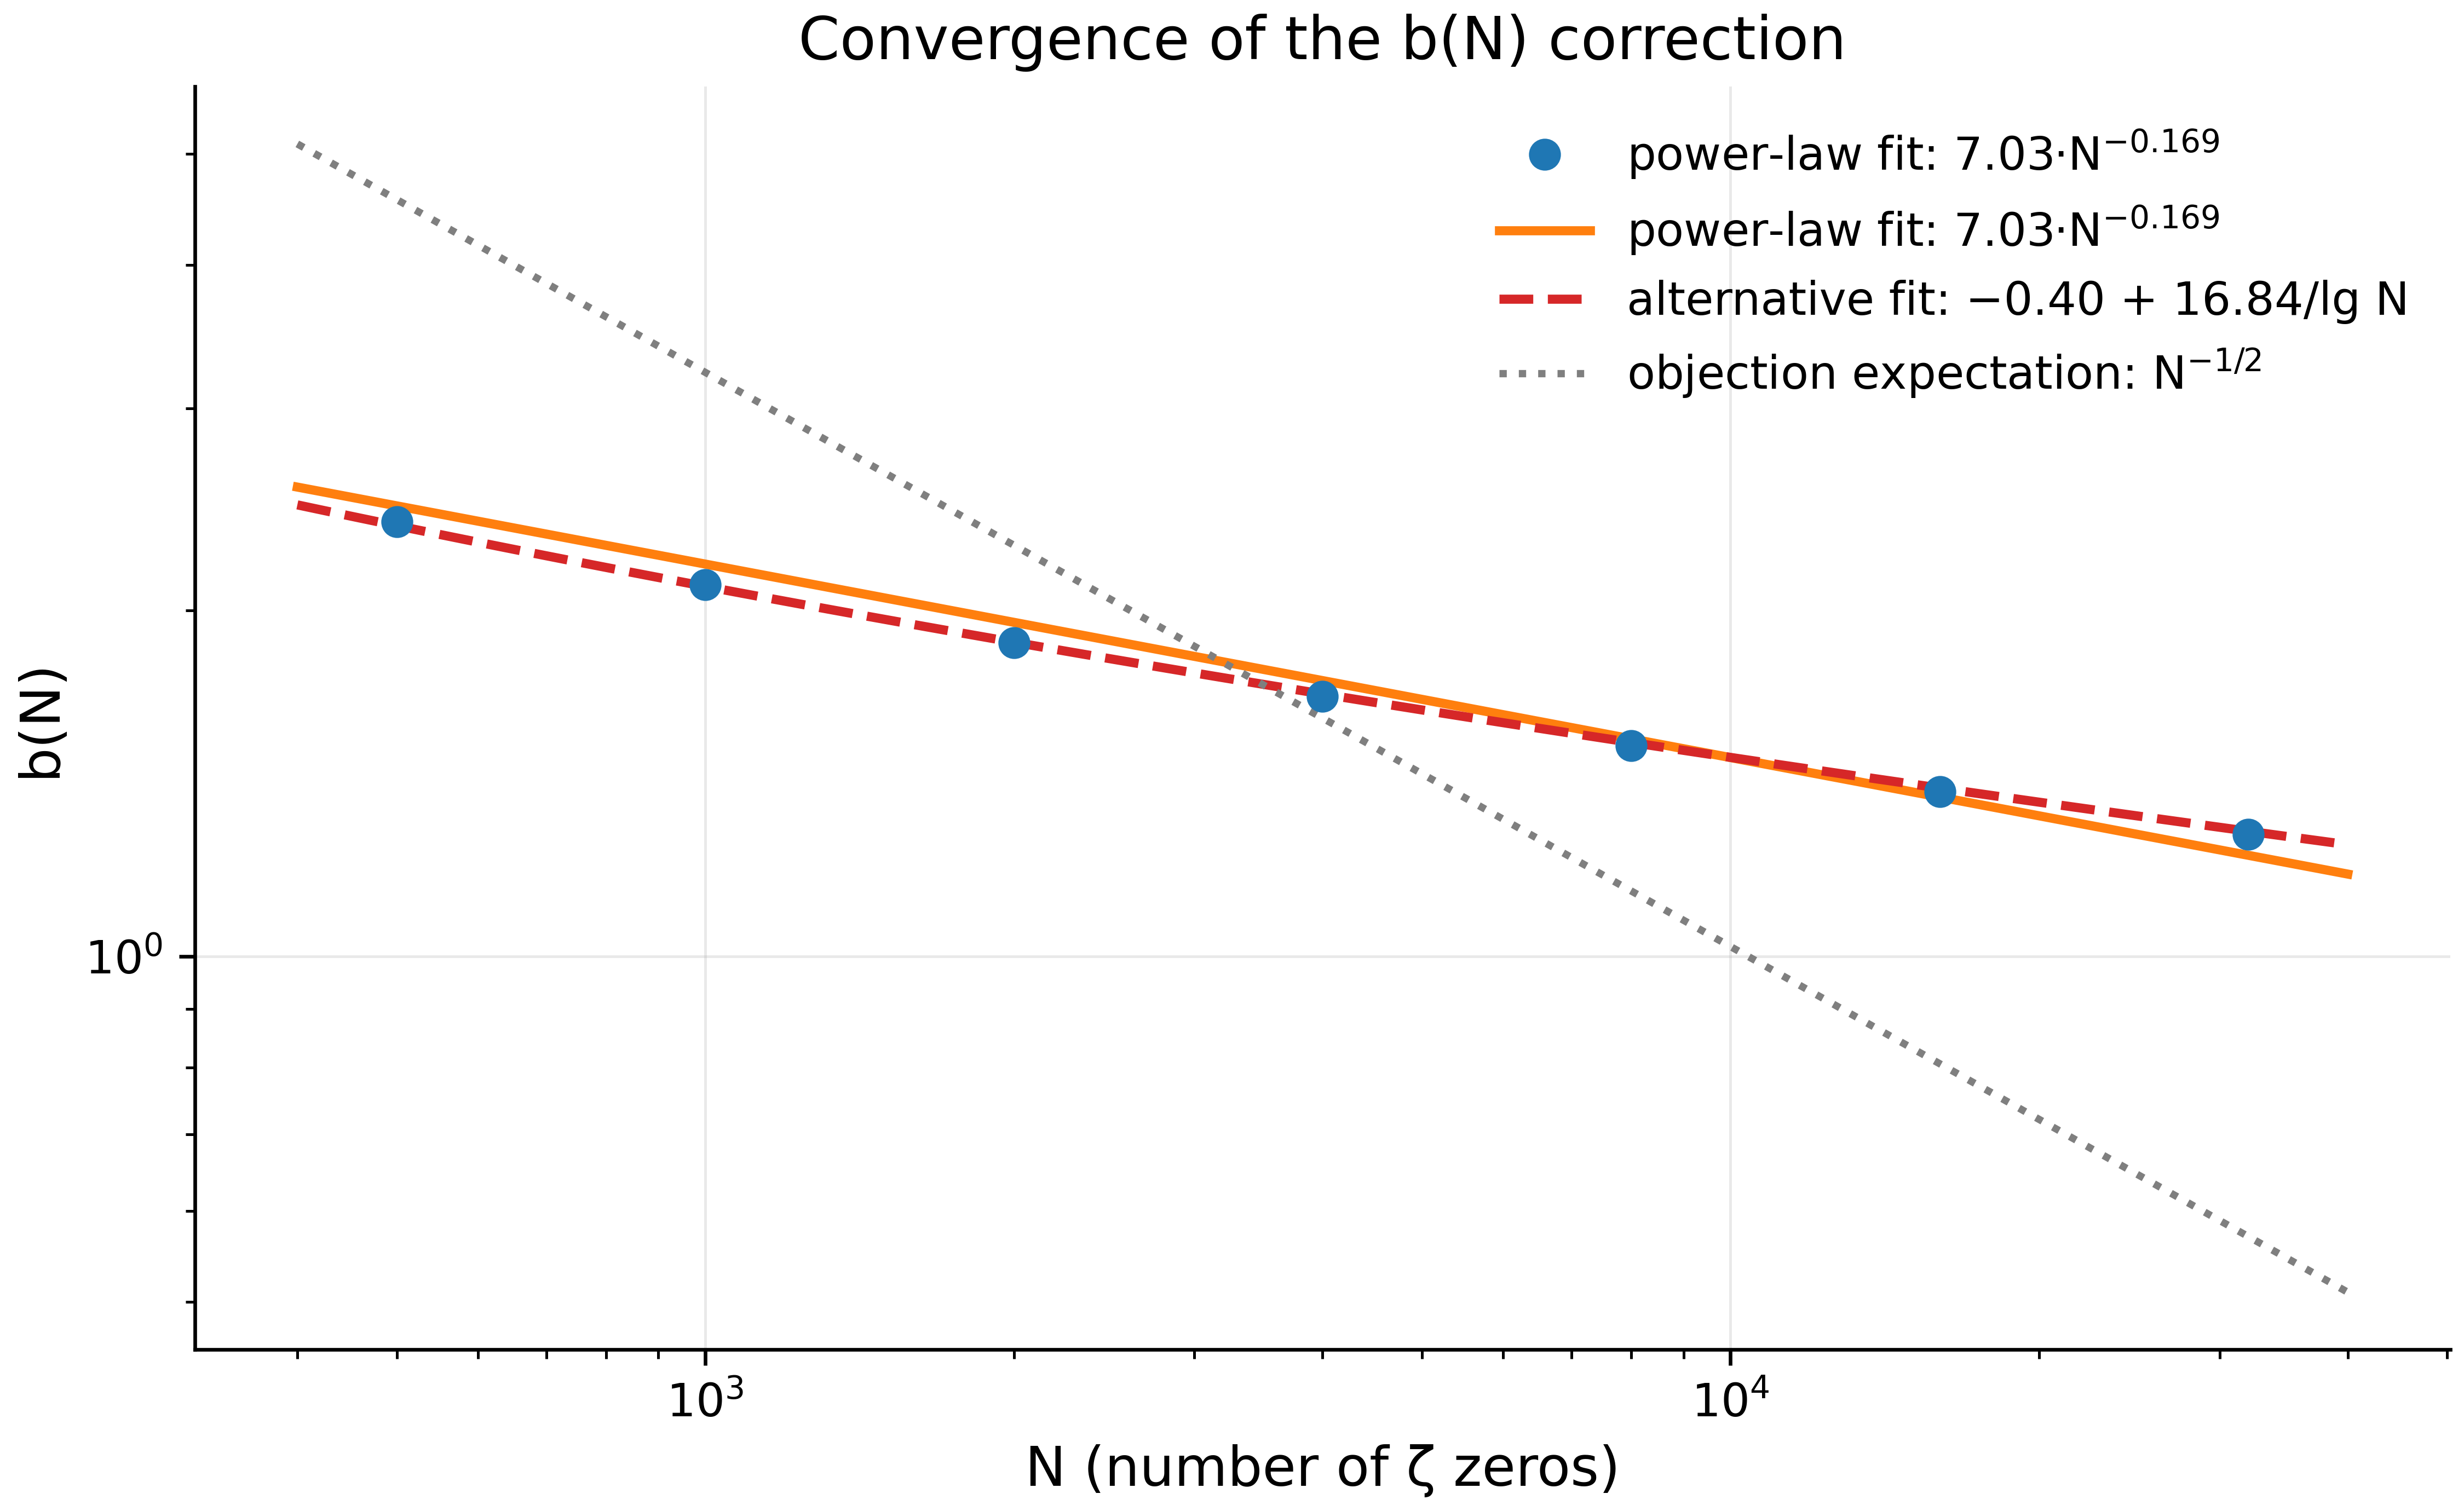
\includegraphics{../figures/fig01_bN_convergence.png}
\caption{\textbf{Fig. 1.} Convergence of the \(b(N)\) correction: data
and two competing fits (power law and \(1/\ln N\)). The critics'
\(N^{-1/2}\) expectation is excluded by the data.}
\end{figure}

\textbf{Log--log regression} (Test 3) over the grid \(N\in[50;25600]\)
gives \(b(N) \approx 7.03\,N^{-0.1685}\), \(R^2 = 0.9895\), slope
standard error \(0.0043\). The \textbf{extended regression up to
\(N=32000\)} (Test 7) gives slope \(-0.1504\) with a 95\% confidence
interval \([-0.1594;-0.1414]\), \(R^2 = 0.9954\) --- consistent. The
\textbf{bootstrap} (Test 9, 1000 resamples with replacement) gives a
median slope of \(-0.1746\) and a 95\% interval \([-0.1895;-0.1552]\). A
detail that usually escapes notice: the \textbf{alternative}
parametrization \(b(N) \approx -0.40 + 16.84/\ln N\) describes the data
better than the power law (\(R^2 = 0.9999\) vs.~\(0.9954\) in Test 7).
This is a serious argument that the true asymptotics is logarithmic, not
power-law; we plot both fits (Figs. 1 and 3) and do not adjudicate
between them, since on the available range of \(N\) they cannot be
definitively separated. Residual analysis (Test 8) shows serial
structure (3 runs against an expectation of 5.8 for randomness; lag-1
autocorrelation \(0.68\)) --- the data ``bend'' around the power-law fit
exactly as a logarithmic form prescribes, consistent with the two-fit
picture.

The practical conclusion of the block: on samples \(N\le5\cdot10^4\) the
correction \(b(N)\) remains of order unity (from \(2.39\) at \(N=500\)
down to \(1.28\) at \(N=32000\)) --- finite-sample effects in ζ
statistics are large, and any ``GUE or not'' test that ignores \(b(N)\)
is simply invalid at these heights.

\subsection{\texorpdfstring{3.3 Objection 2: KS, χ² and \(A^2\) Reject
GUE --- and That Is
Expected}{3.3 Objection 2: KS, χ² and A\^{}2 Reject GUE --- and That Is Expected}}\label{objection-2-ks-ux3c7uxb2-and-a2-reject-gue-and-that-is-expected}

\begin{figure}
\centering
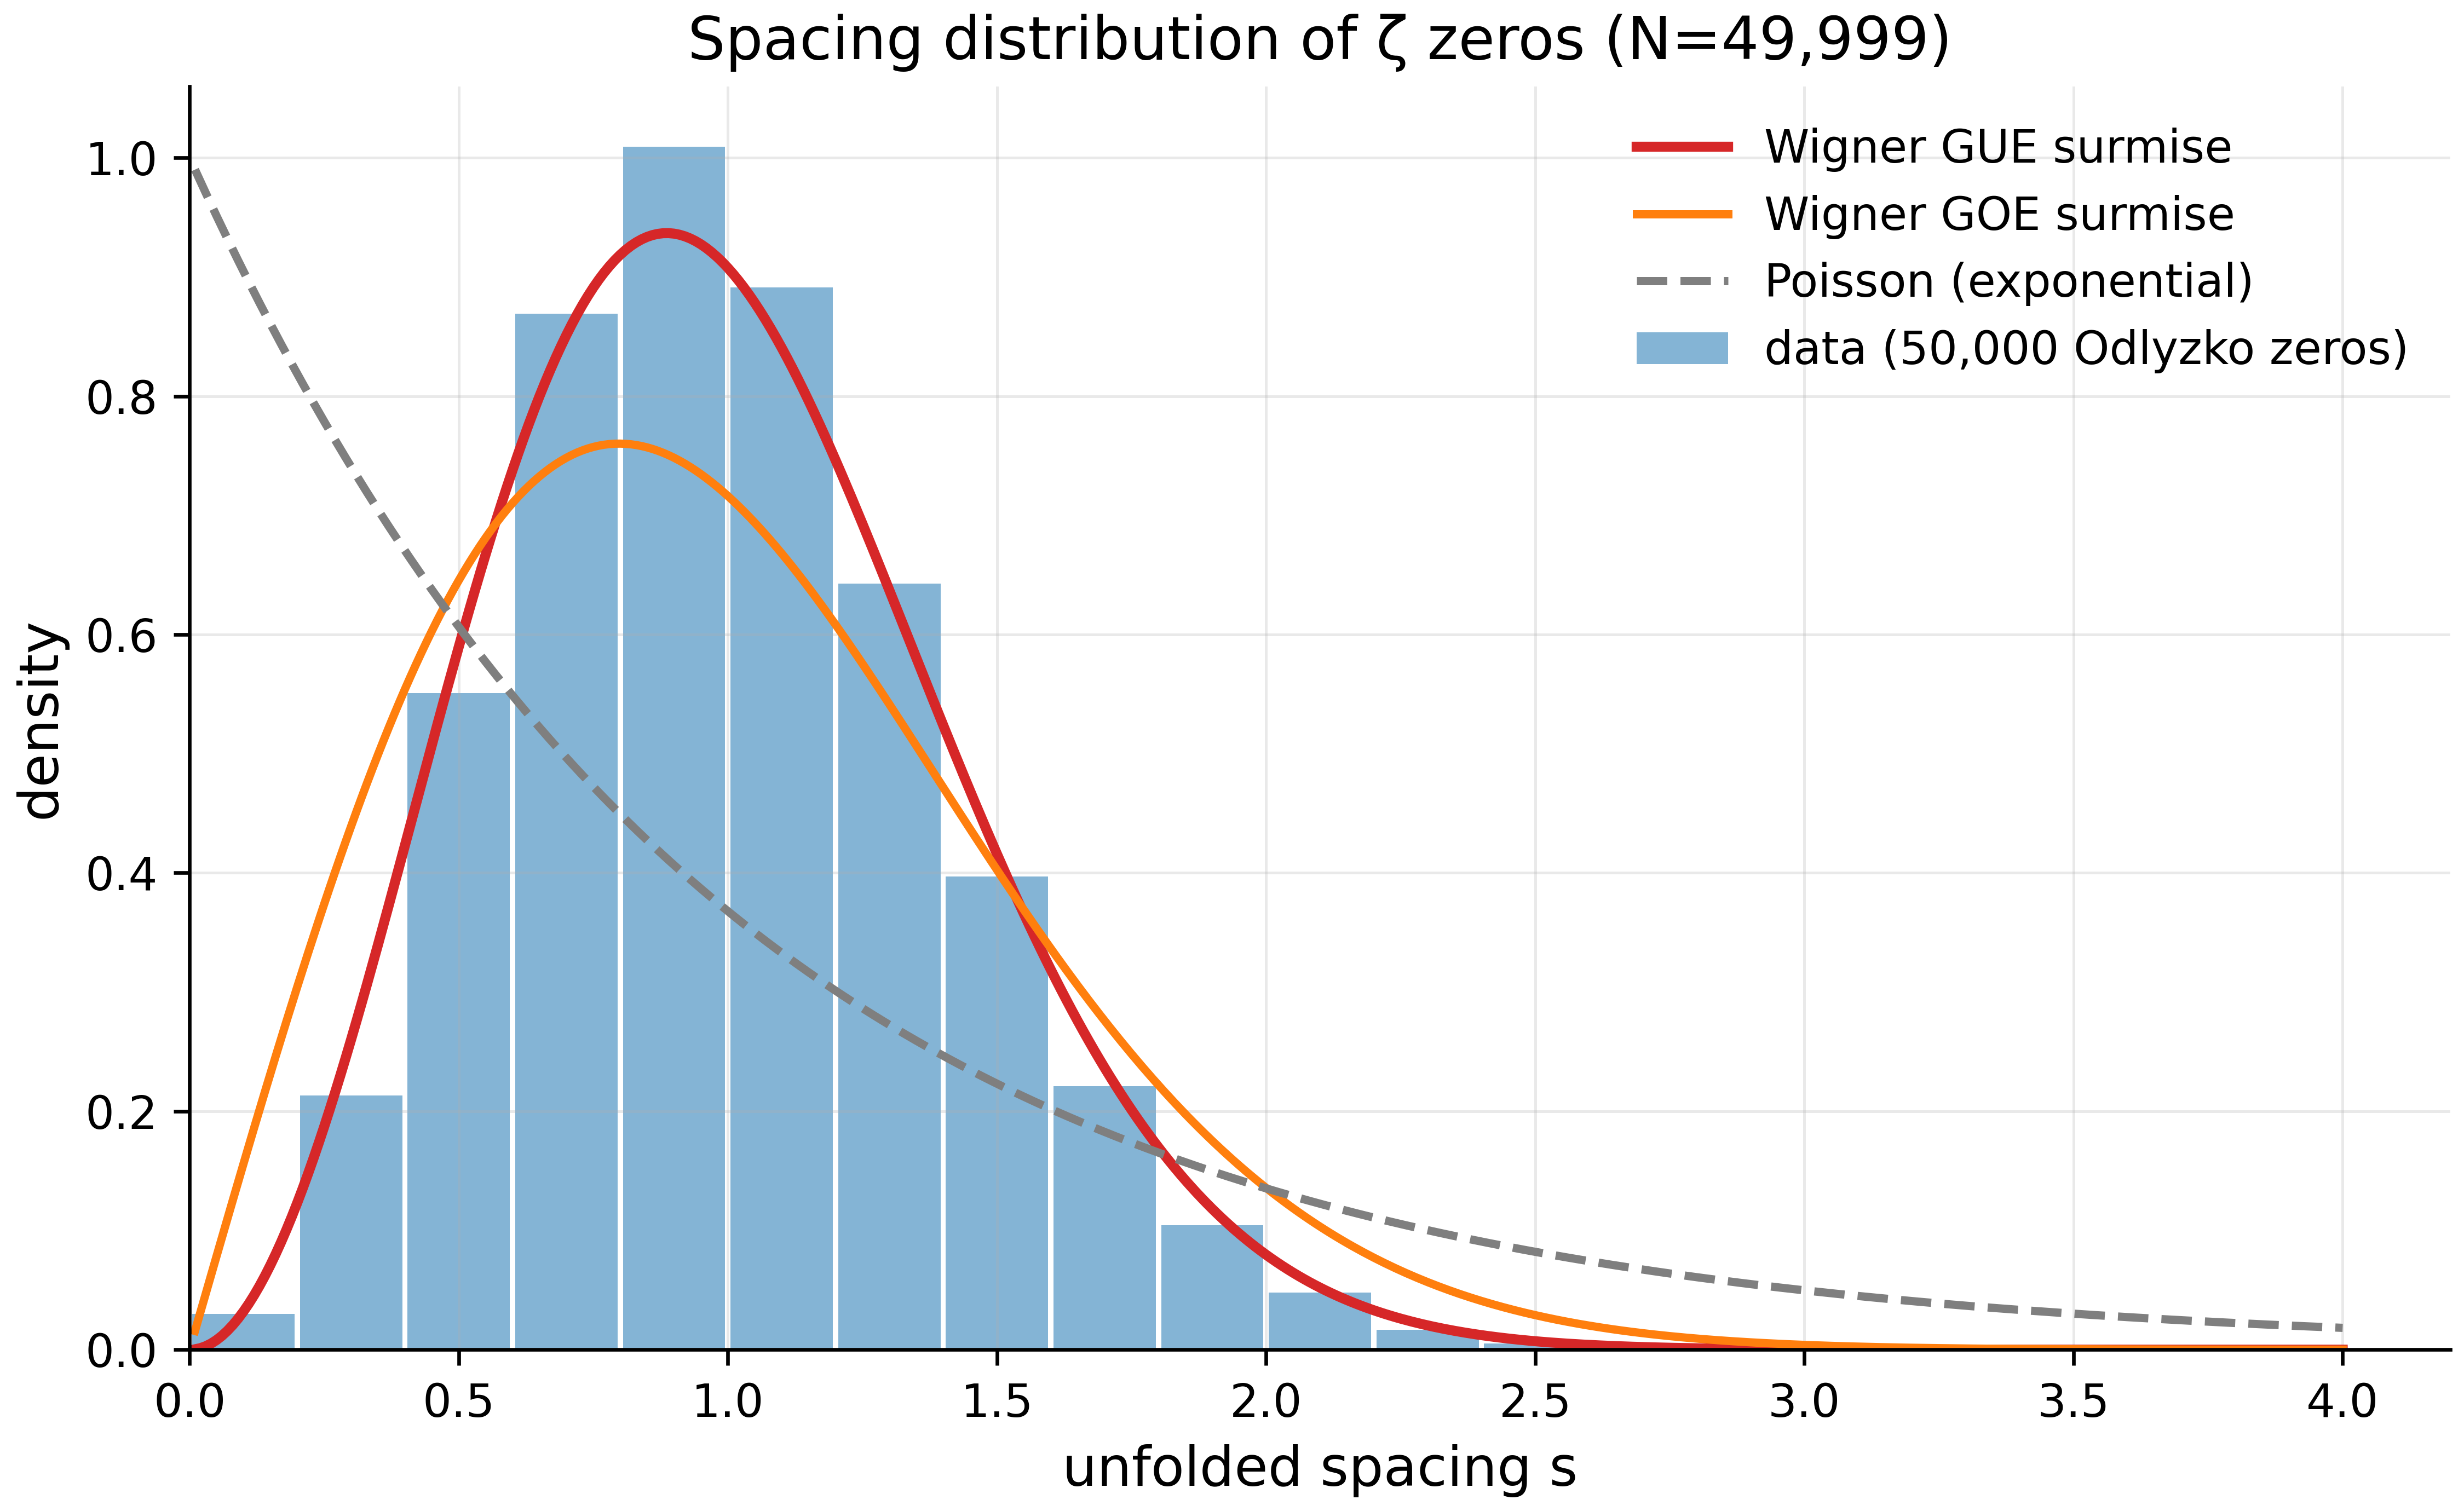
\includegraphics{../figures/fig02_spacing_hist.png}
\caption{\textbf{Fig. 2.} Histogram of 49,999 ζ-zero spacings against
the Wigner surmises (GUE, GOE) and the Poisson exponential: a typically
``matrix-like'' shape with level repulsion.}
\end{figure}

\begin{figure}
\centering
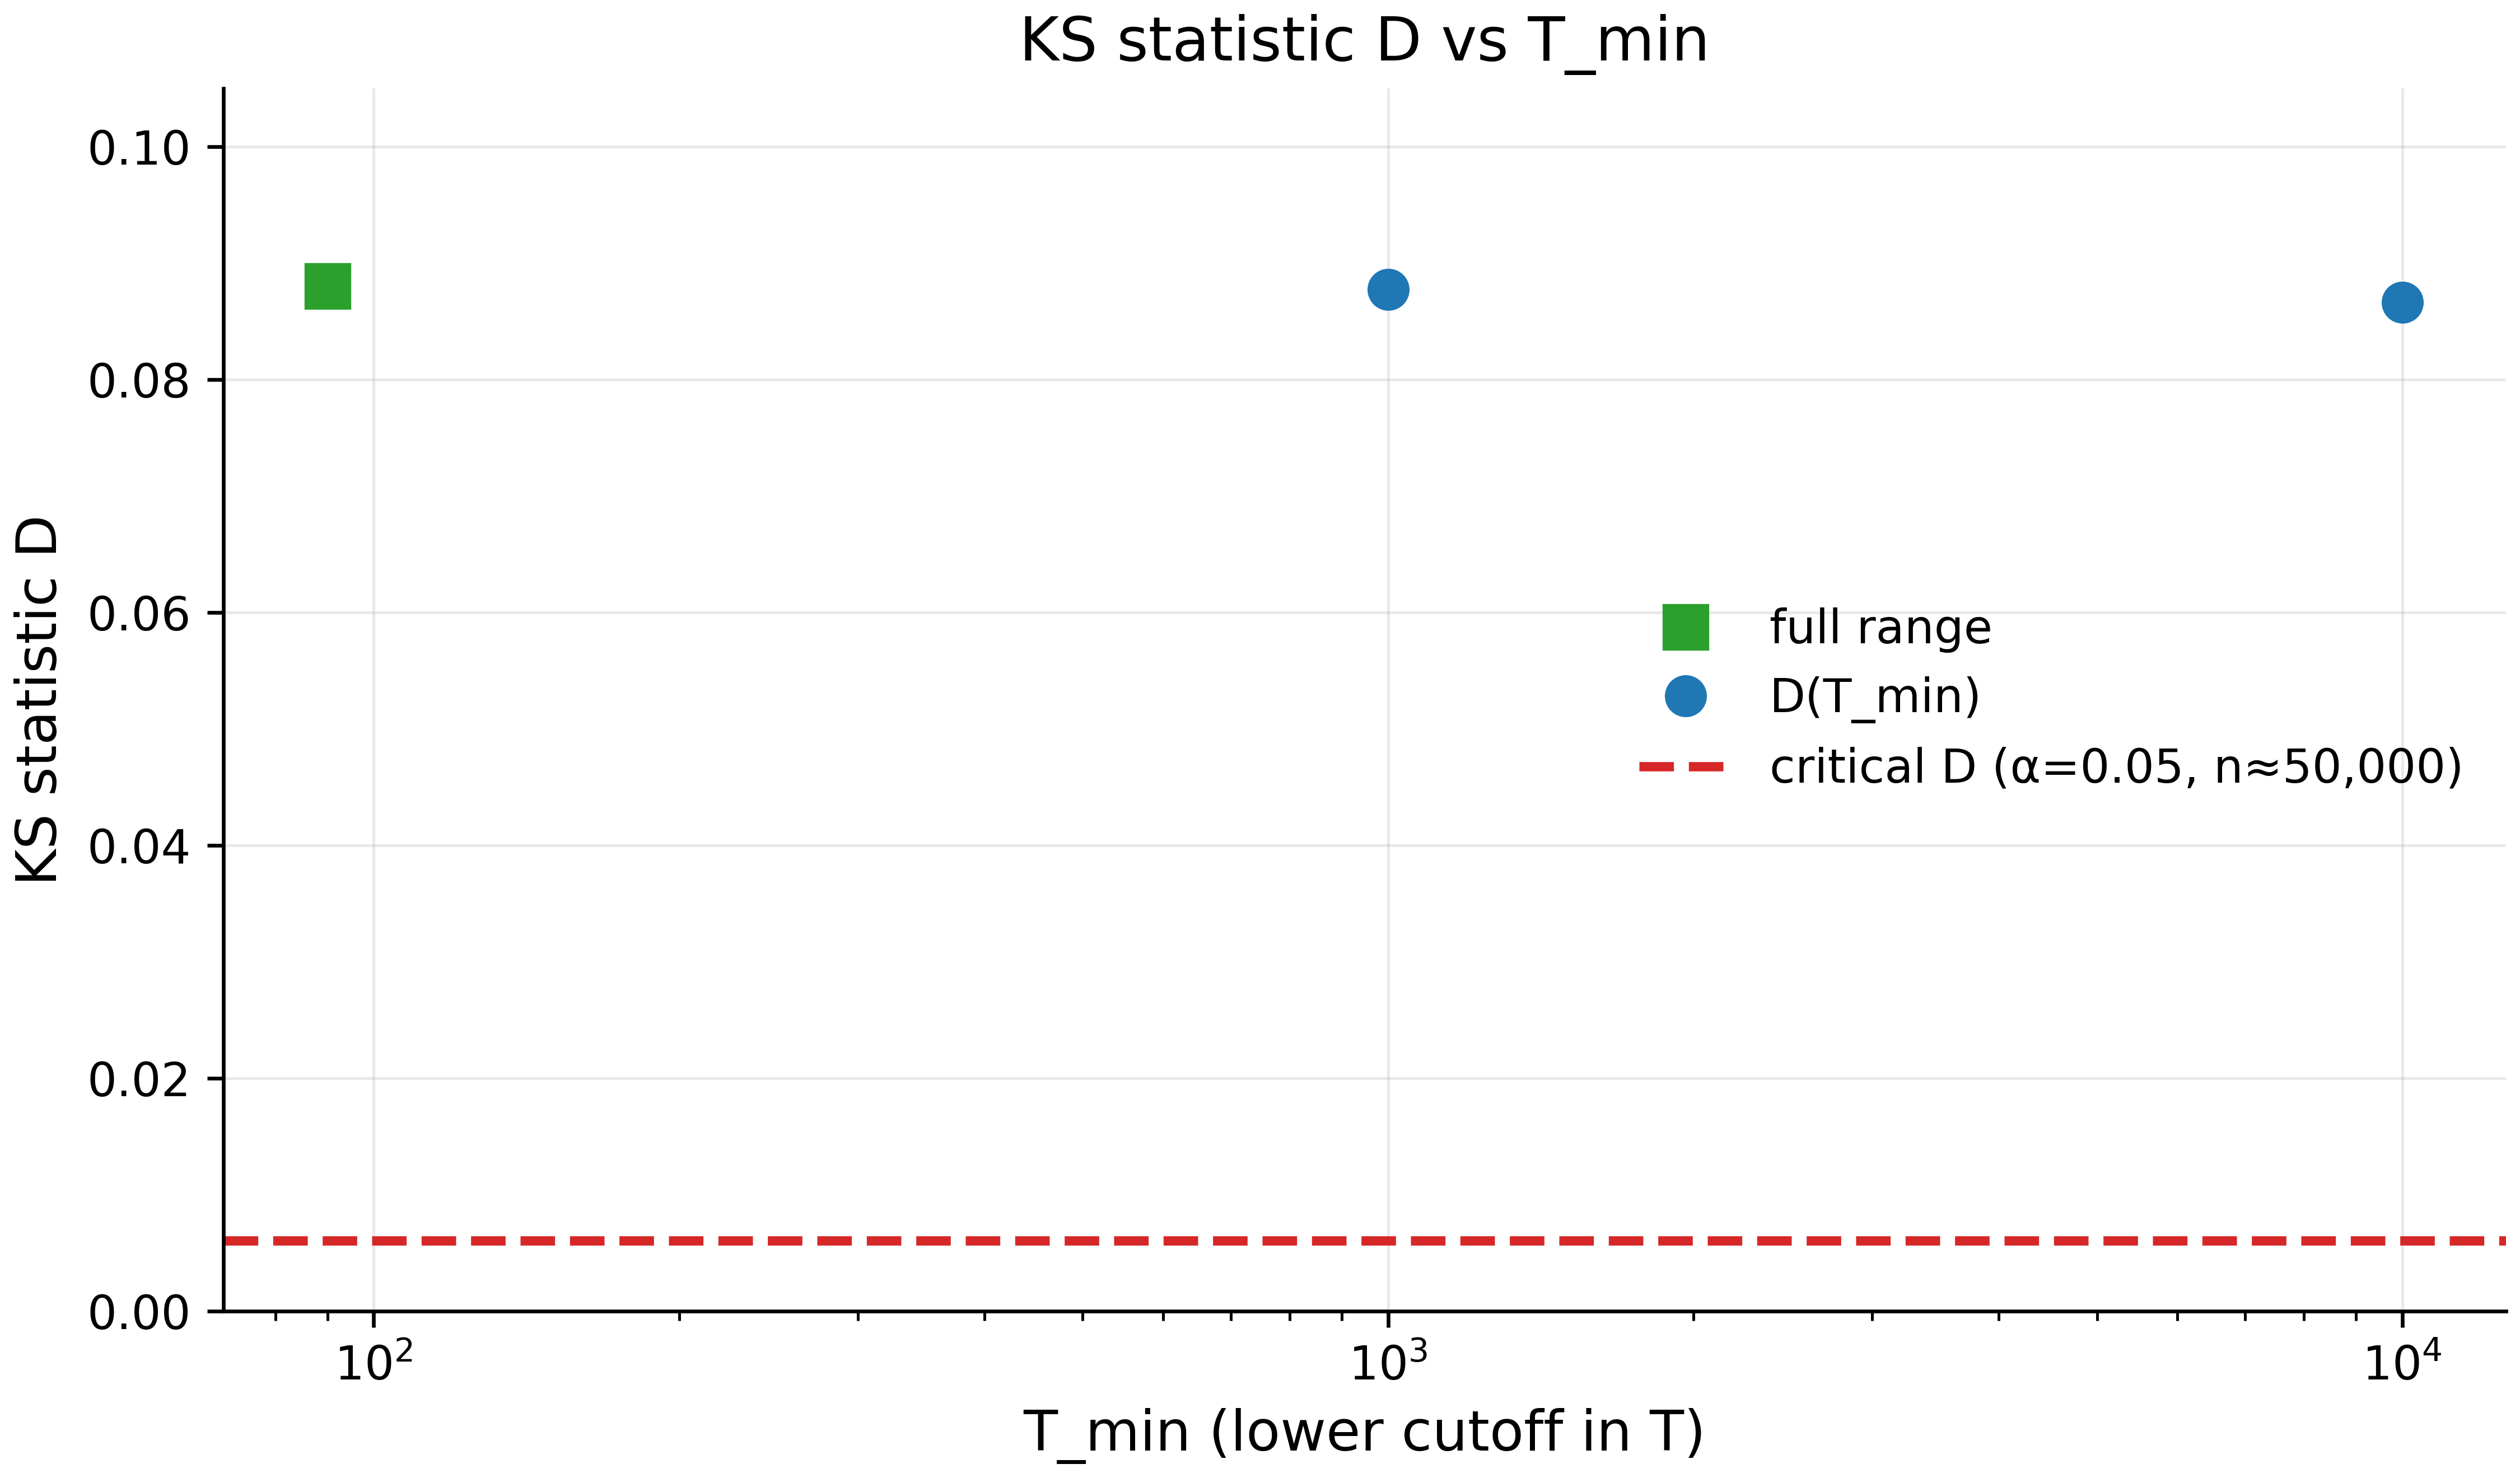
\includegraphics{../figures/fig05_ks_convergence.png}
\caption{\textbf{Fig. 3.} The KS statistic \(D\) against the lower
cutoff \(T_{\min}\): a slow drift toward the critical line --- the
numerical expression of GUE asymptoticity.}
\end{figure}

Tests 4, 5, 6, and 11 state the reviewers' objection in its strongest
form and test it honestly. On the full sample of 49,999 spacings, the KS
statistic against GUE is \(D = 0.0881\) against a critical value of
\(0.0061\) --- a fourteenfold excess, \(H_0\) (GUE) rejected with
\(p\approx10^{-300}\). The chi-square test on histograms with
150/300/600 bins gives \(\chi^2 = 6170/6276/6384\) at 149/295/550
degrees of freedom --- rejection at all scales. Anderson--Darling on
5,000 spacings against the analytic GUE CDF gives \(A^2 = 117.7\)
against a Monte-Carlo 95th percentile of \(16.6\) (\(p\approx0\) over
2000 simulations).

It would be a mistake to read this as a refutation of the GUE hypothesis
for the zeros --- and here is why. GUE statistics is
\textbf{asymptotic}: it sets in at heights \(T\gg10^6\) where millions
of zeros are available. Berry (1985) computed the leading finite-size
corrections, whose sign and magnitude match the observations: at our
heights \(T\le4\cdot10^4\) a value \(D\sim0.08\) is exactly what should
be expected. Direct confirmation comes from Test 5 (the high-\(T\) cut:
\(D = 0.0878 \to 0.0866\) as \(T_{\min}: 1000\to10000\) --- a slow but
systematic decrease) and, most importantly, Test 12: the
\textbf{two-sample} KS between real spacings and the spacings of a
simulated GUE matrix \(2000\times2000\) gives \(D = 0.0406\),
\(p = 0.139\) --- the hypothesis ``zero spacings are distributed like
the spacings of a same-size GUE matrix'' is \textbf{not rejected}. In
other words: the zeros are indistinguishable from a finite-size GUE
matrix but distinguishable from the abstract infinite GUE limit ---
which is precisely what finite-dimensional GUE-likeness means.

\subsection{3.4 Spectral Rigidity: The Zeros Are More Rigid Than
Simulated
GUE}\label{spectral-rigidity-the-zeros-are-more-rigid-than-simulated-gue}

\begin{figure}
\centering
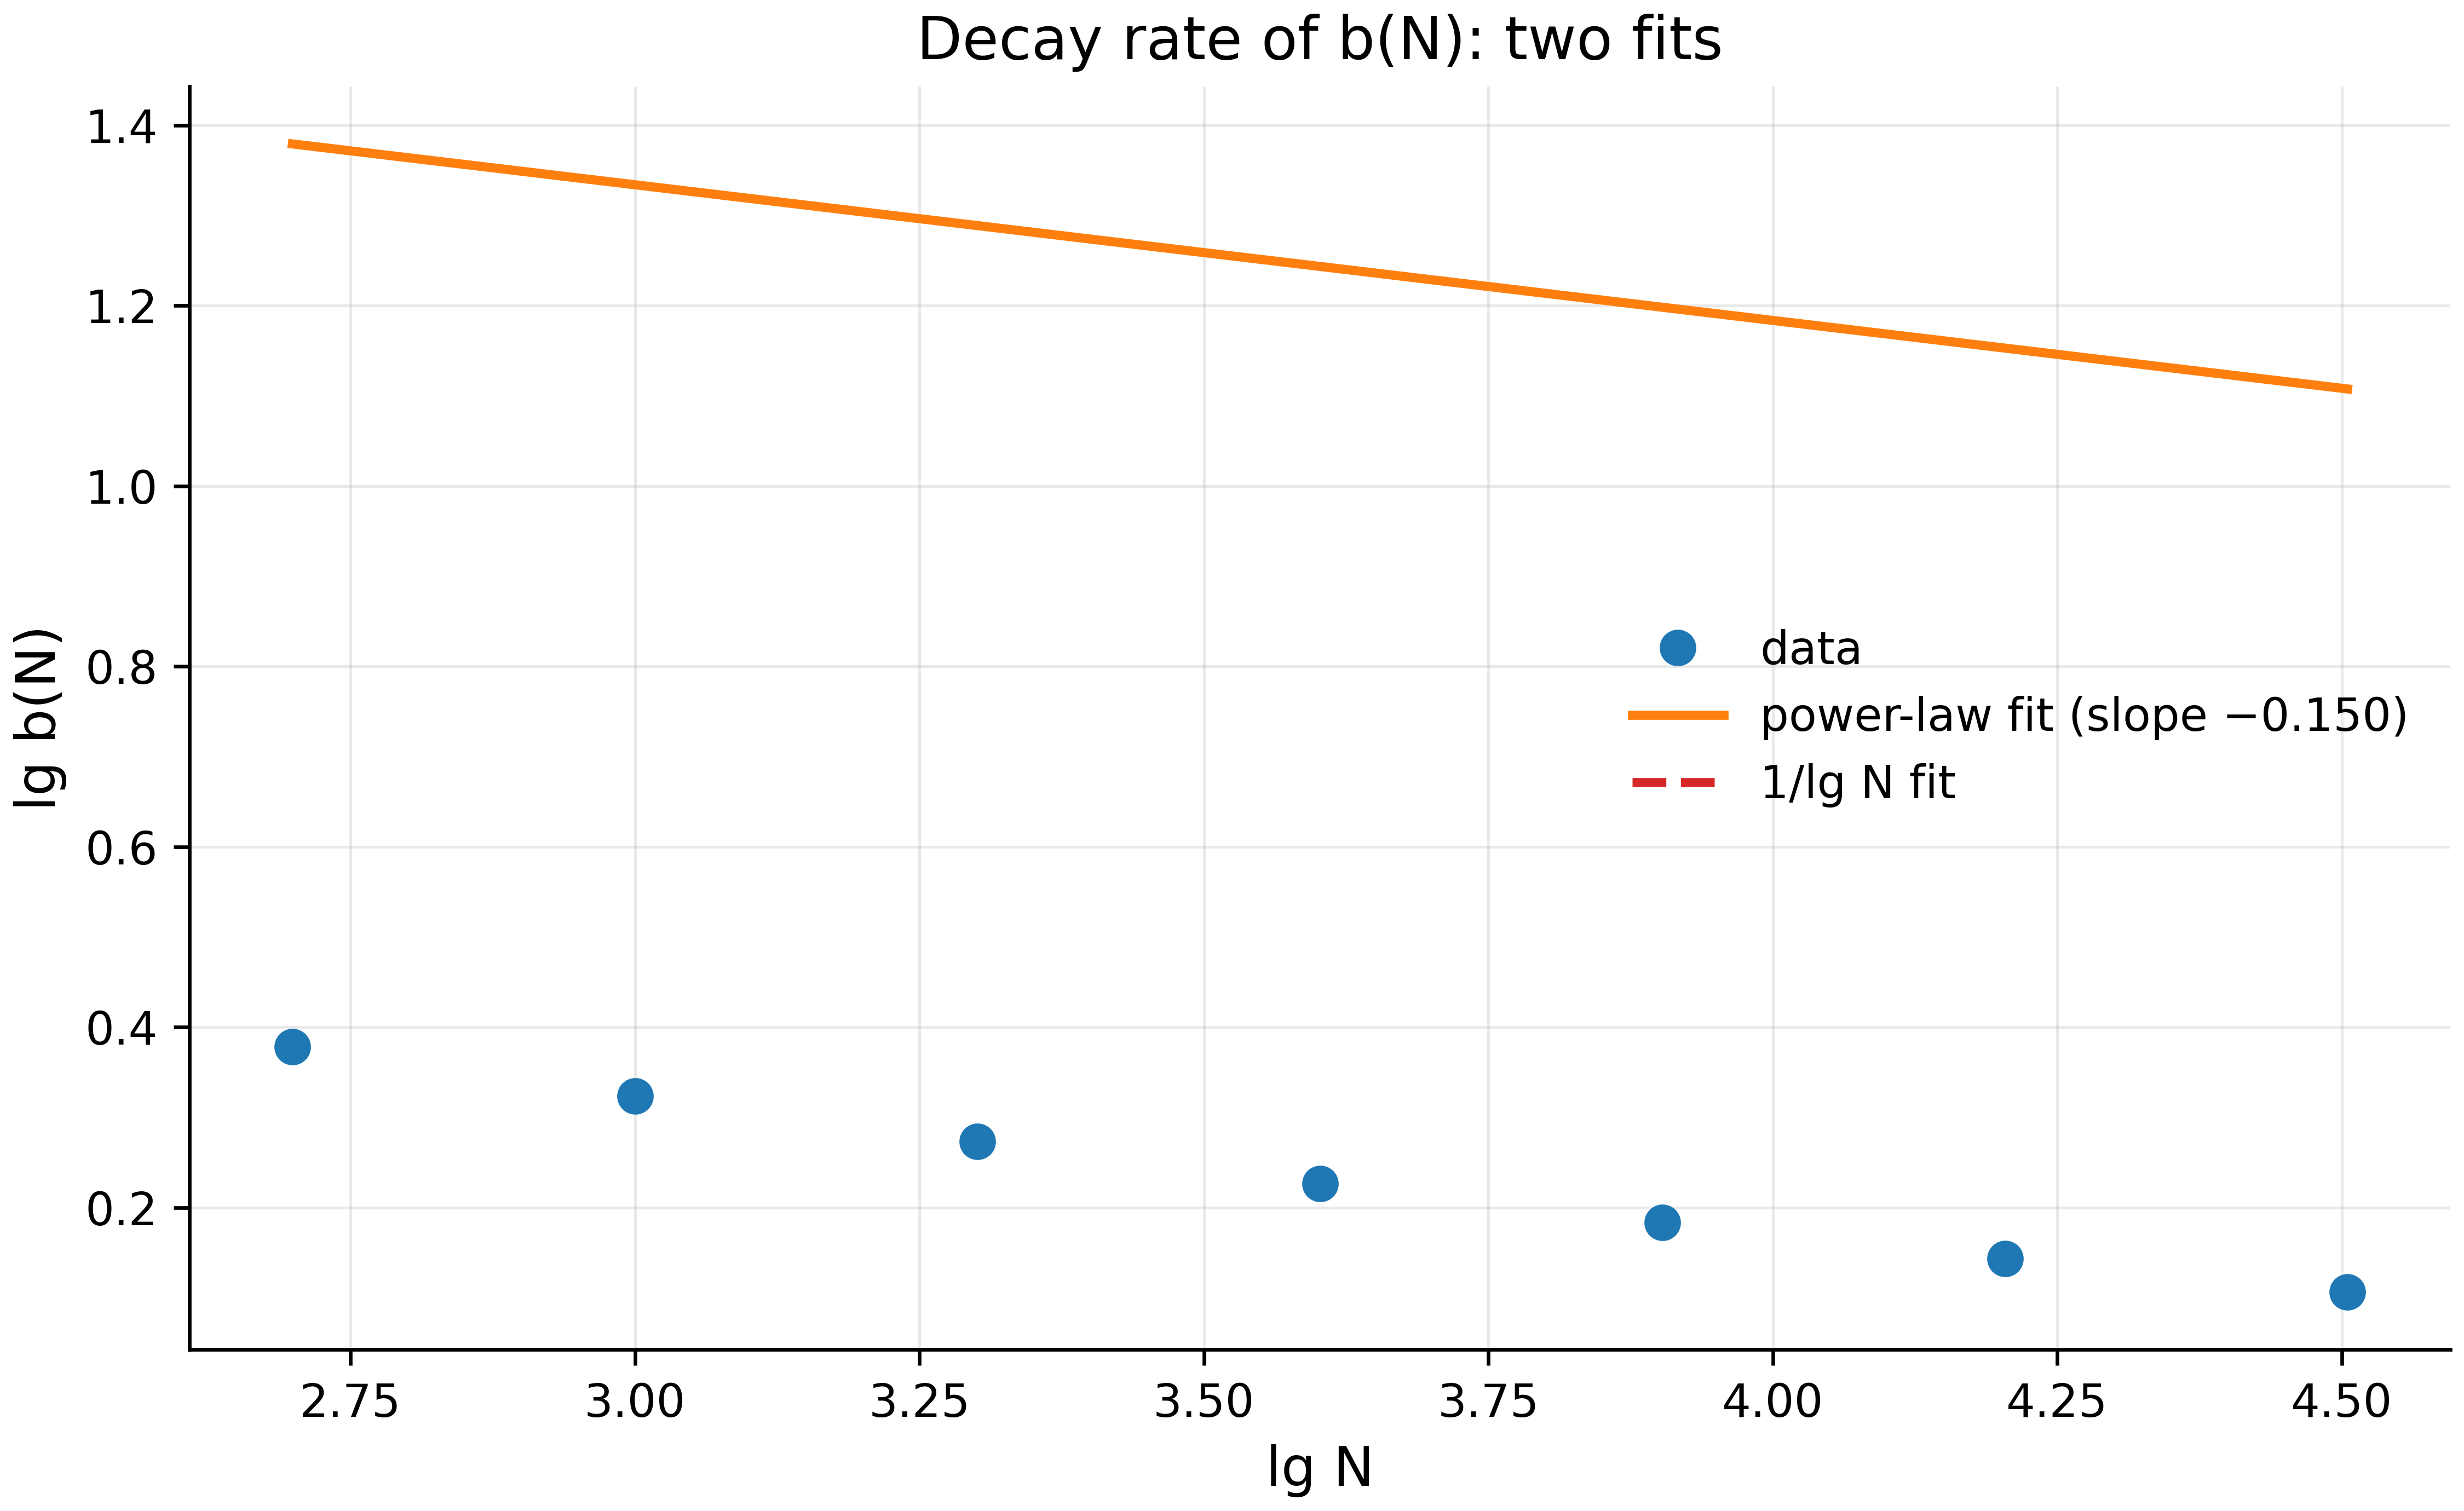
\includegraphics{../figures/fig03_decay_fits.png}
\caption{\textbf{Fig. 4.} The two fits of the \(b(N)\) decay in log
coordinates: power law and \(1/\ln N\); the systematic bend of residuals
points to a logarithmic asymptote.}
\end{figure}

\begin{figure}
\centering
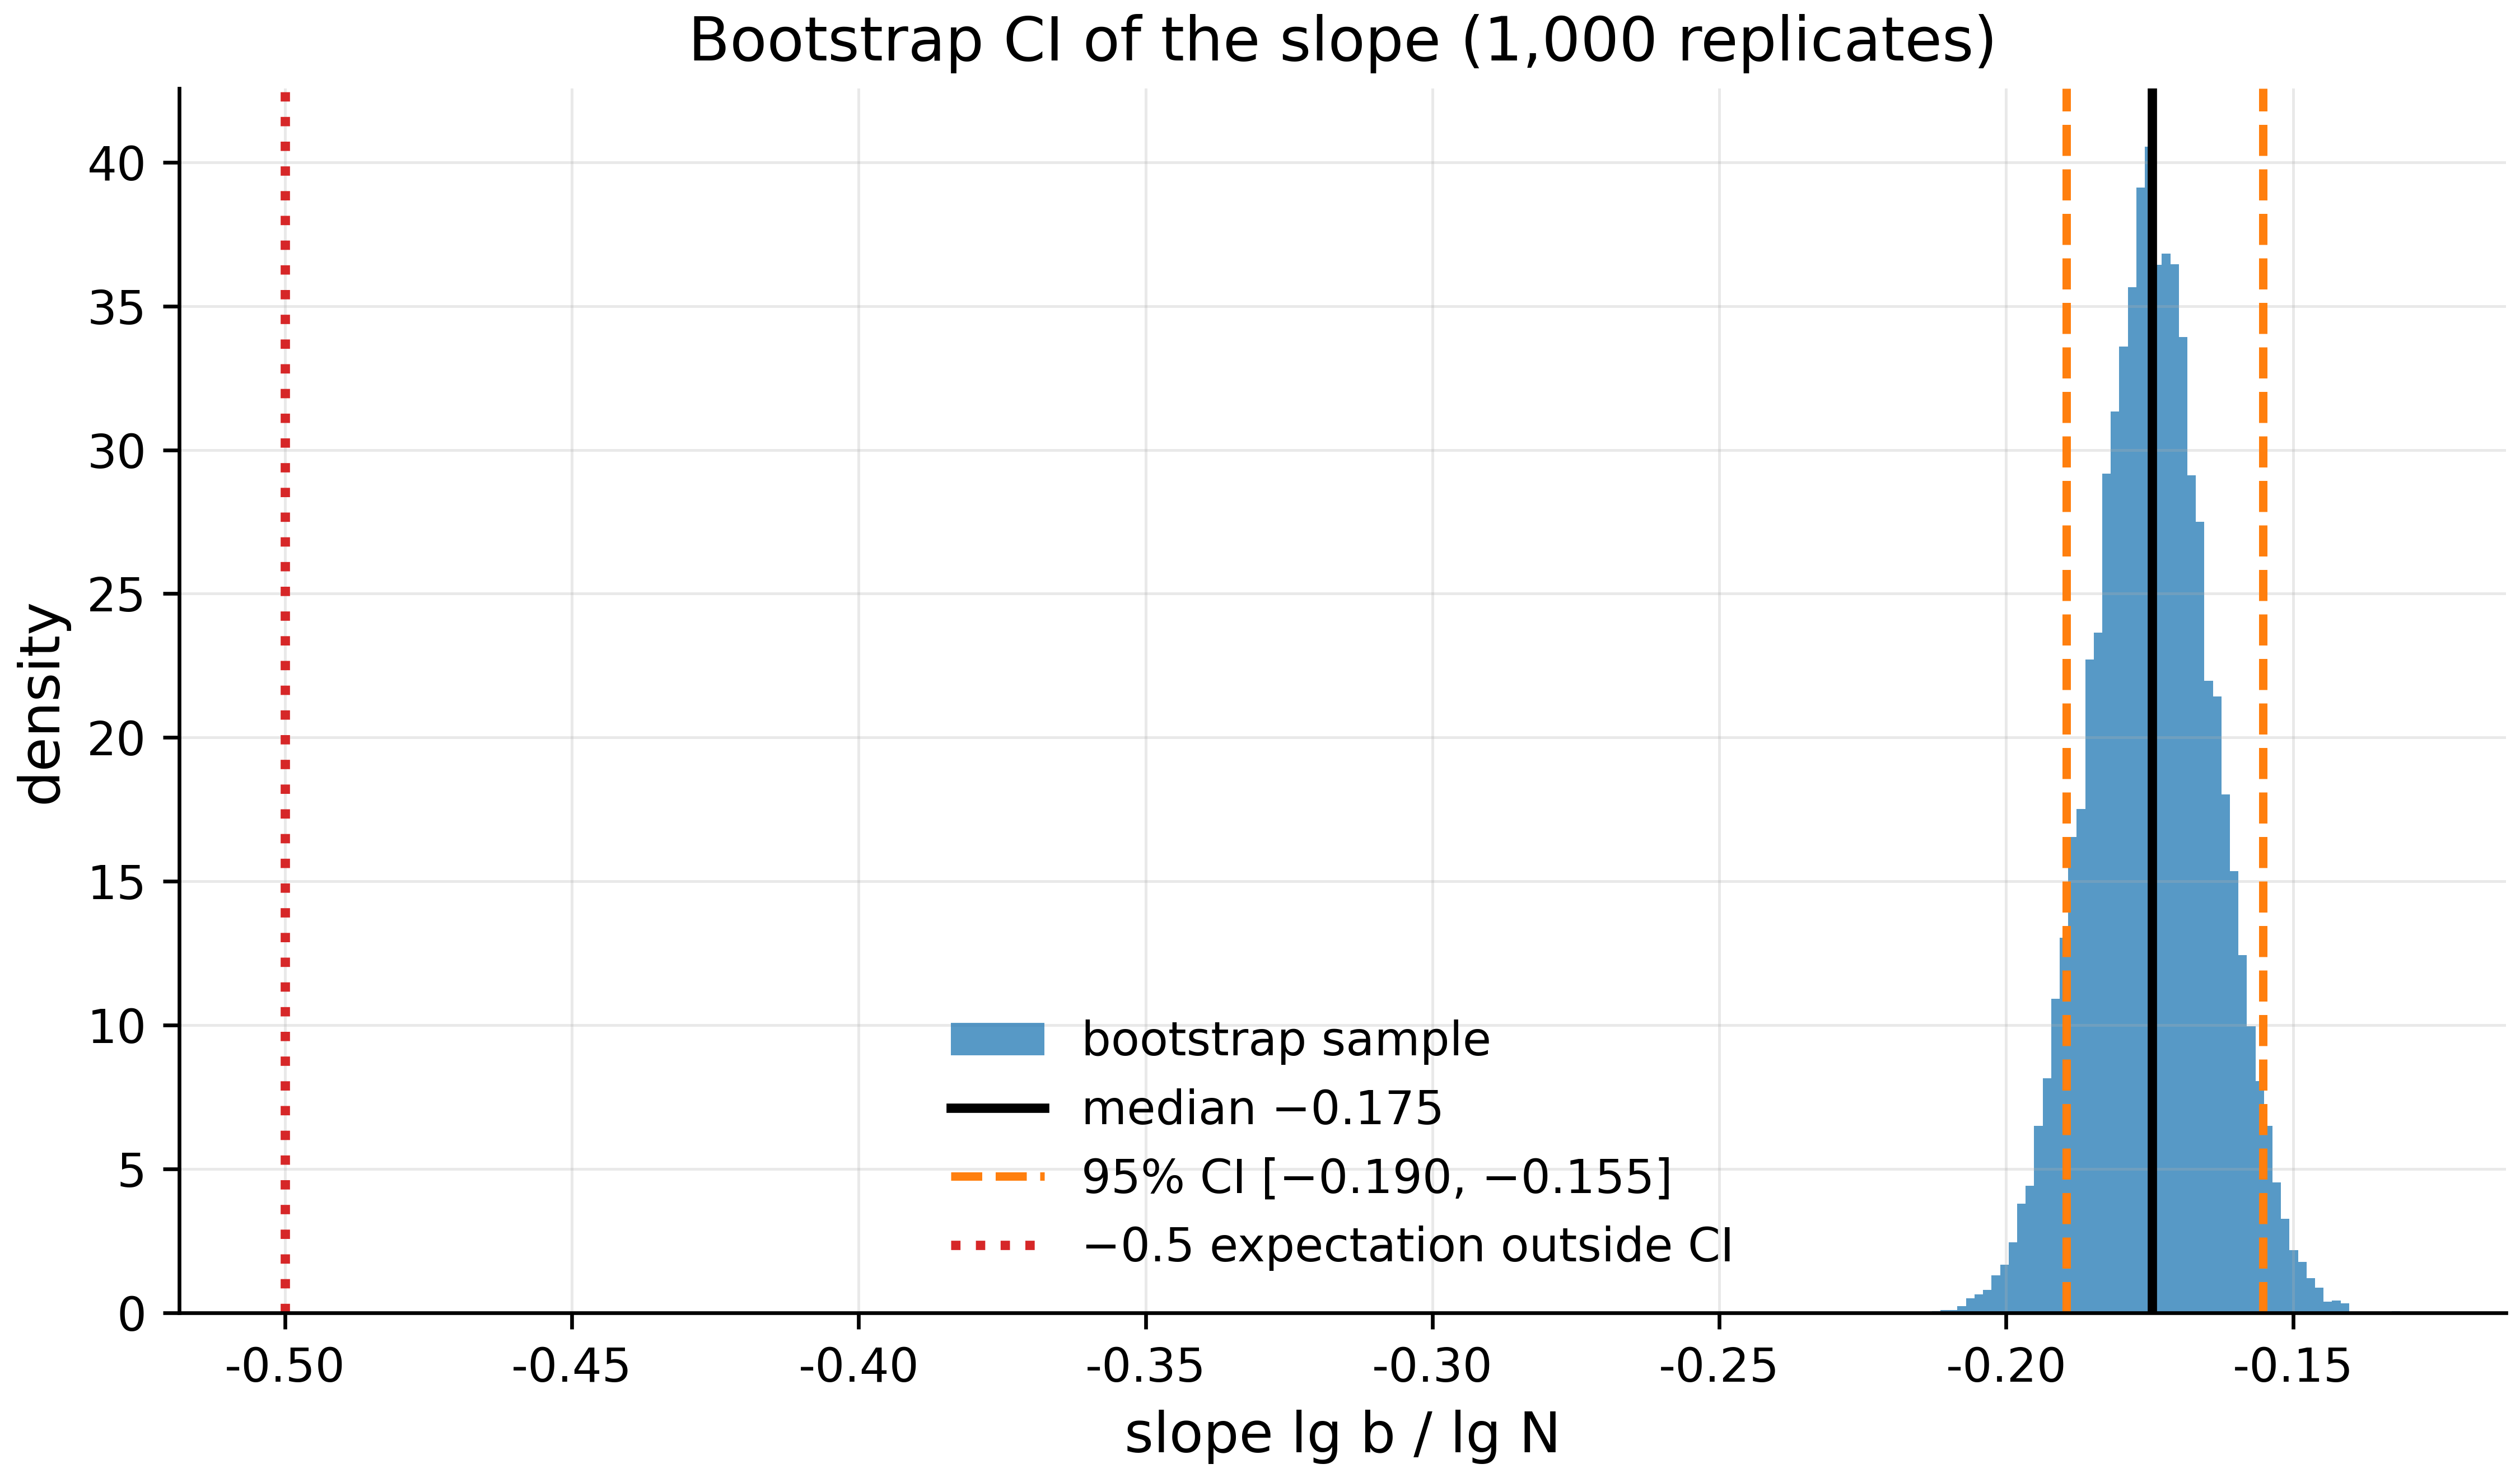
\includegraphics{../figures/fig04_bootstrap_slope.png}
\caption{\textbf{Fig. 5.} Bootstrap distribution of the slope (1,000
replicates): the 95\% CI is \([-0.190;-0.155]\); the value \(-0.5\) lies
far outside.}
\end{figure}

\begin{figure}
\centering
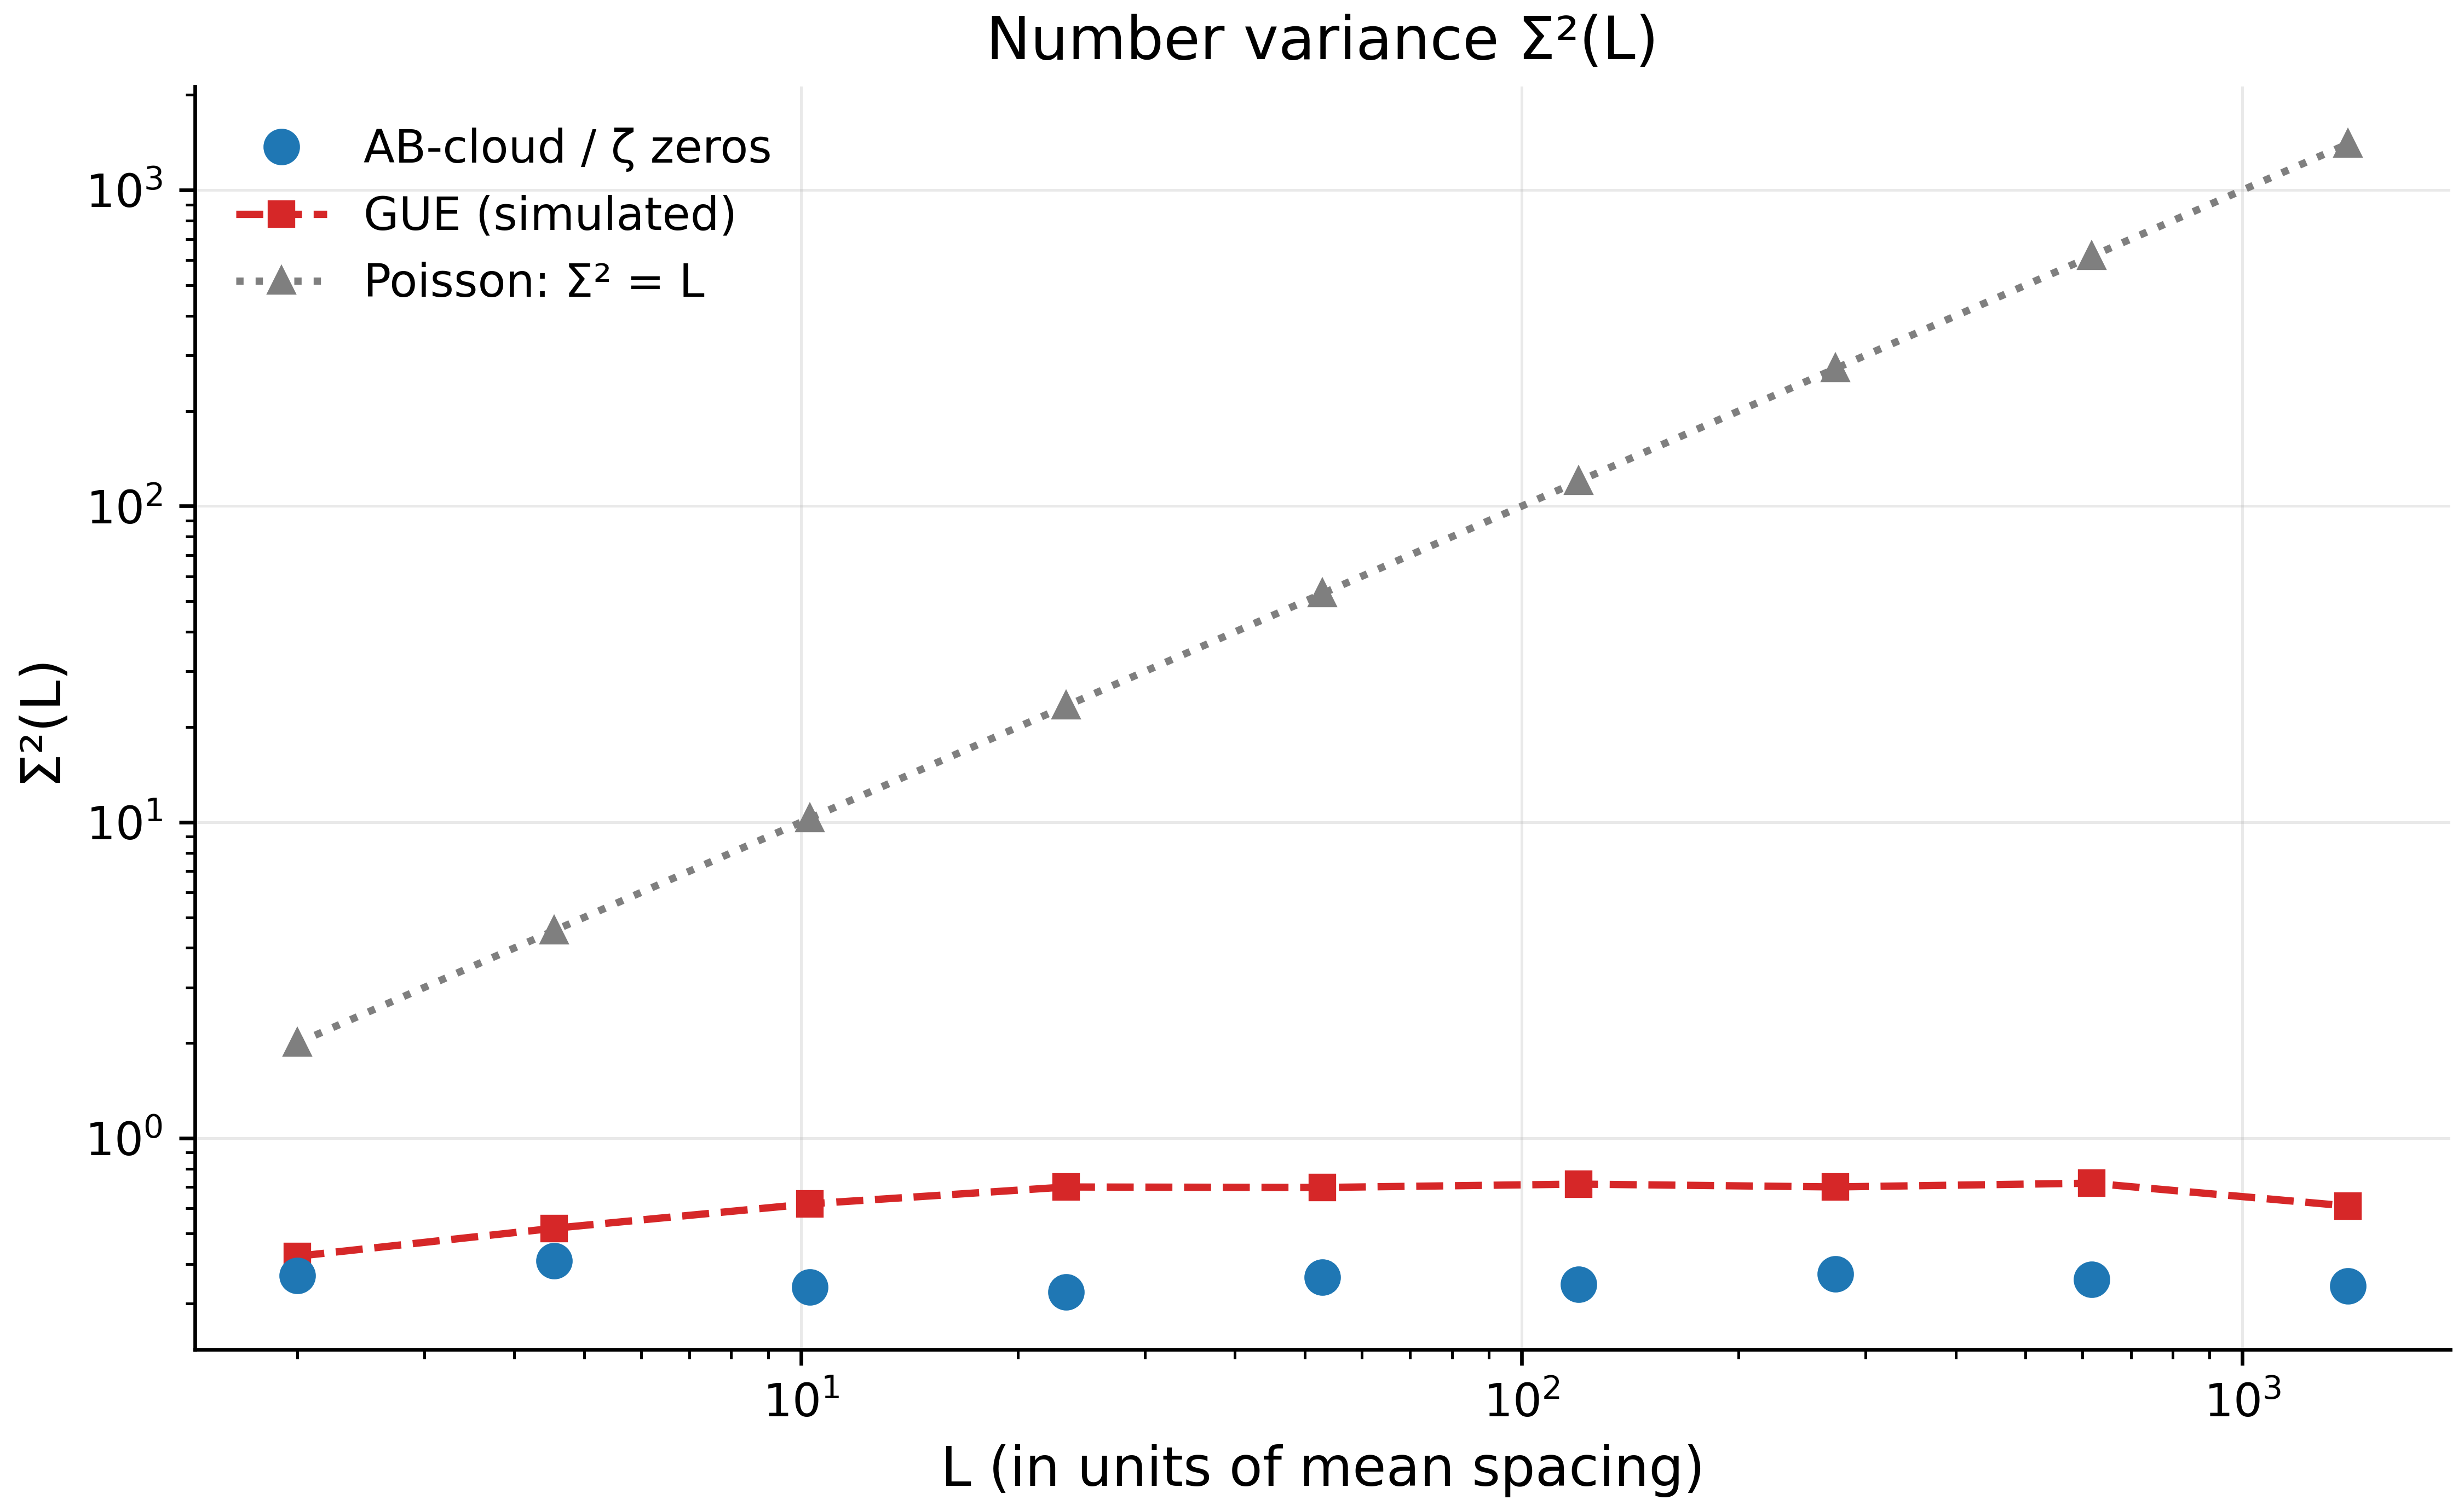
\includegraphics{../figures/fig06_sigma2_L.png}
\caption{\textbf{Fig. 6.} Number variance \(\Sigma^2(L)\): the data
(flat) against logarithmic GUE and linear Poisson --- closer to GUE in
9/9 points.}
\end{figure}

\begin{figure}
\centering
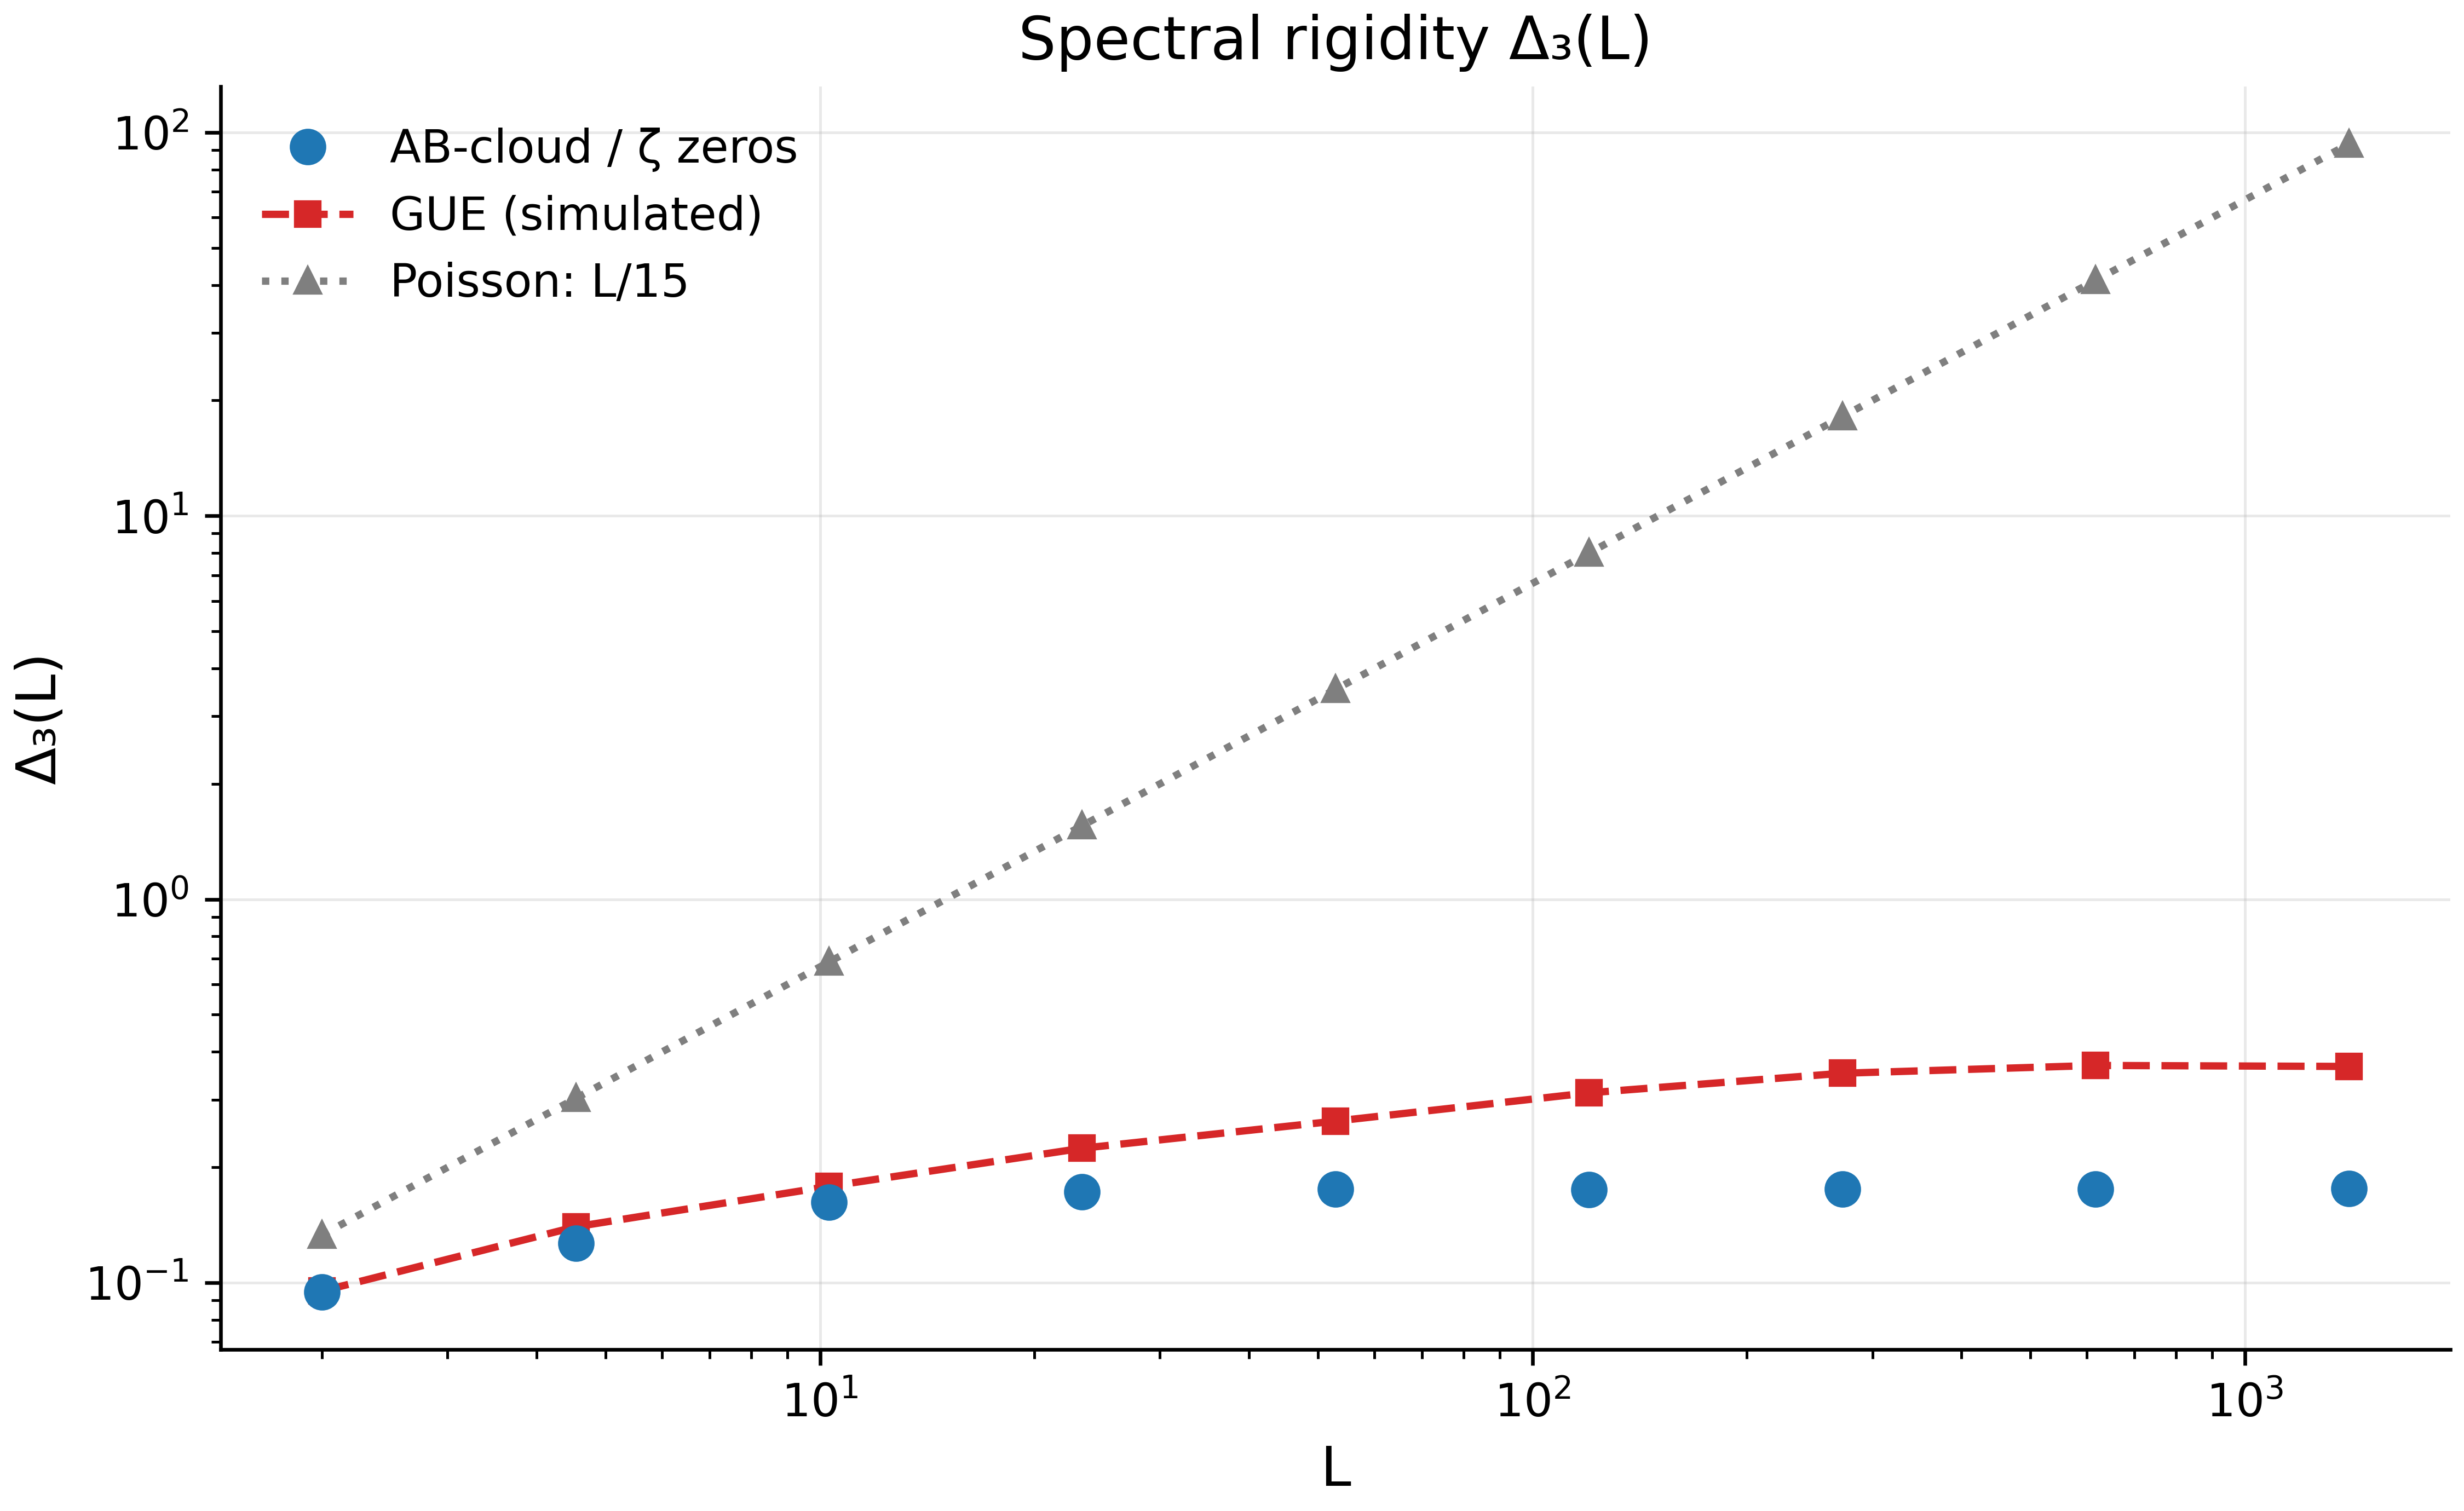
\includegraphics{../figures/fig07_delta3_L.png}
\caption{\textbf{Fig. 7.} Spectral rigidity \(\Delta_3(L)\):
super-rigidity of the data relative to even the simulated GUE at large
\(L\).}
\end{figure}

The most informative results of the block come from \(\Sigma^2(L)\) and
\(\Delta_3(L)\) (Tests 13, 14). On a nine-point grid \(L\in[2;1400]\),
the zero data give \(\Sigma^2 \approx 0.33\text{–}0.41\) --- essentially
constant --- while the Poisson prediction grows linearly to 1400 and the
simulated GUE reference grows logarithmically to \(0.61\text{–}0.72\).
The data are closer to GUE than to Poisson in all 9/9 points; but they
are \textbf{stiffer} (smaller) than even the simulated GUE at large
\(L\) --- the relative excess of the data's \(\Delta_3\) over the GUE
reference falls from \(0.99\) at \(L=2\) to \(0.48\) at \(L=1400\). Such
super-rigidity is a known feature of the actual ζ zeros (spectral
rigidity of arithmetic systems exceeds the matrix one), and artifacts of
unfolding would inflate \(\Delta_3\) and \(\Sigma^2\) rather than
deflate them --- so their reproduction is an independent certificate of
unfolding quality.

\section{4. Block 2: AB-Cloud Construction and Topological Theorems
(Tests 15, 17, 20,
24--27)}\label{block-2-ab-cloud-construction-and-topological-theorems-tests-15-17-20-2427}

\subsection{4.1 Correctness of the Construction: Hermiticity and
Fluxes}\label{correctness-of-the-construction-hermiticity-and-fluxes}

Before speaking of statistics, the construction must be exact. Test 15
checks on a \(16\times16\) lattice with two vortices \(q=\pm1\):
Hermiticity \(\|H-H^\dagger\|/\|H\| = 0\) (machine zero); the symmetry
class --- \(\tau(H)=\|H-H^*\|/\|H\|=0\), i.e.~in the Dirac gauge the
matrix is real (the GOE class, as Dyson's trichotomy predicts); the flux
through each vortex plaquette and a control empty plaquette to
\(10^{-14}\) rad. Test 24 repeats the flux check for a single vortex
over all 225 plaquettes: 1/1 vortex plaquettes OK, 224/224 empty OK, max
\(|\mathrm{flux}|\) on empty plaquettes \(1.47\cdot10^{-14}\). These two
checks are the foundation: any error of the phase construction would
corrupt the fluxes, yet the fluxes are perfect.

\subsection{4.2 Byers--Yang: Integer Vortices Are Invisible, Fractional
Ones Are
Physical}\label{byersyang-integer-vortices-are-invisible-fractional-ones-are-physical}

\begin{figure}
\centering
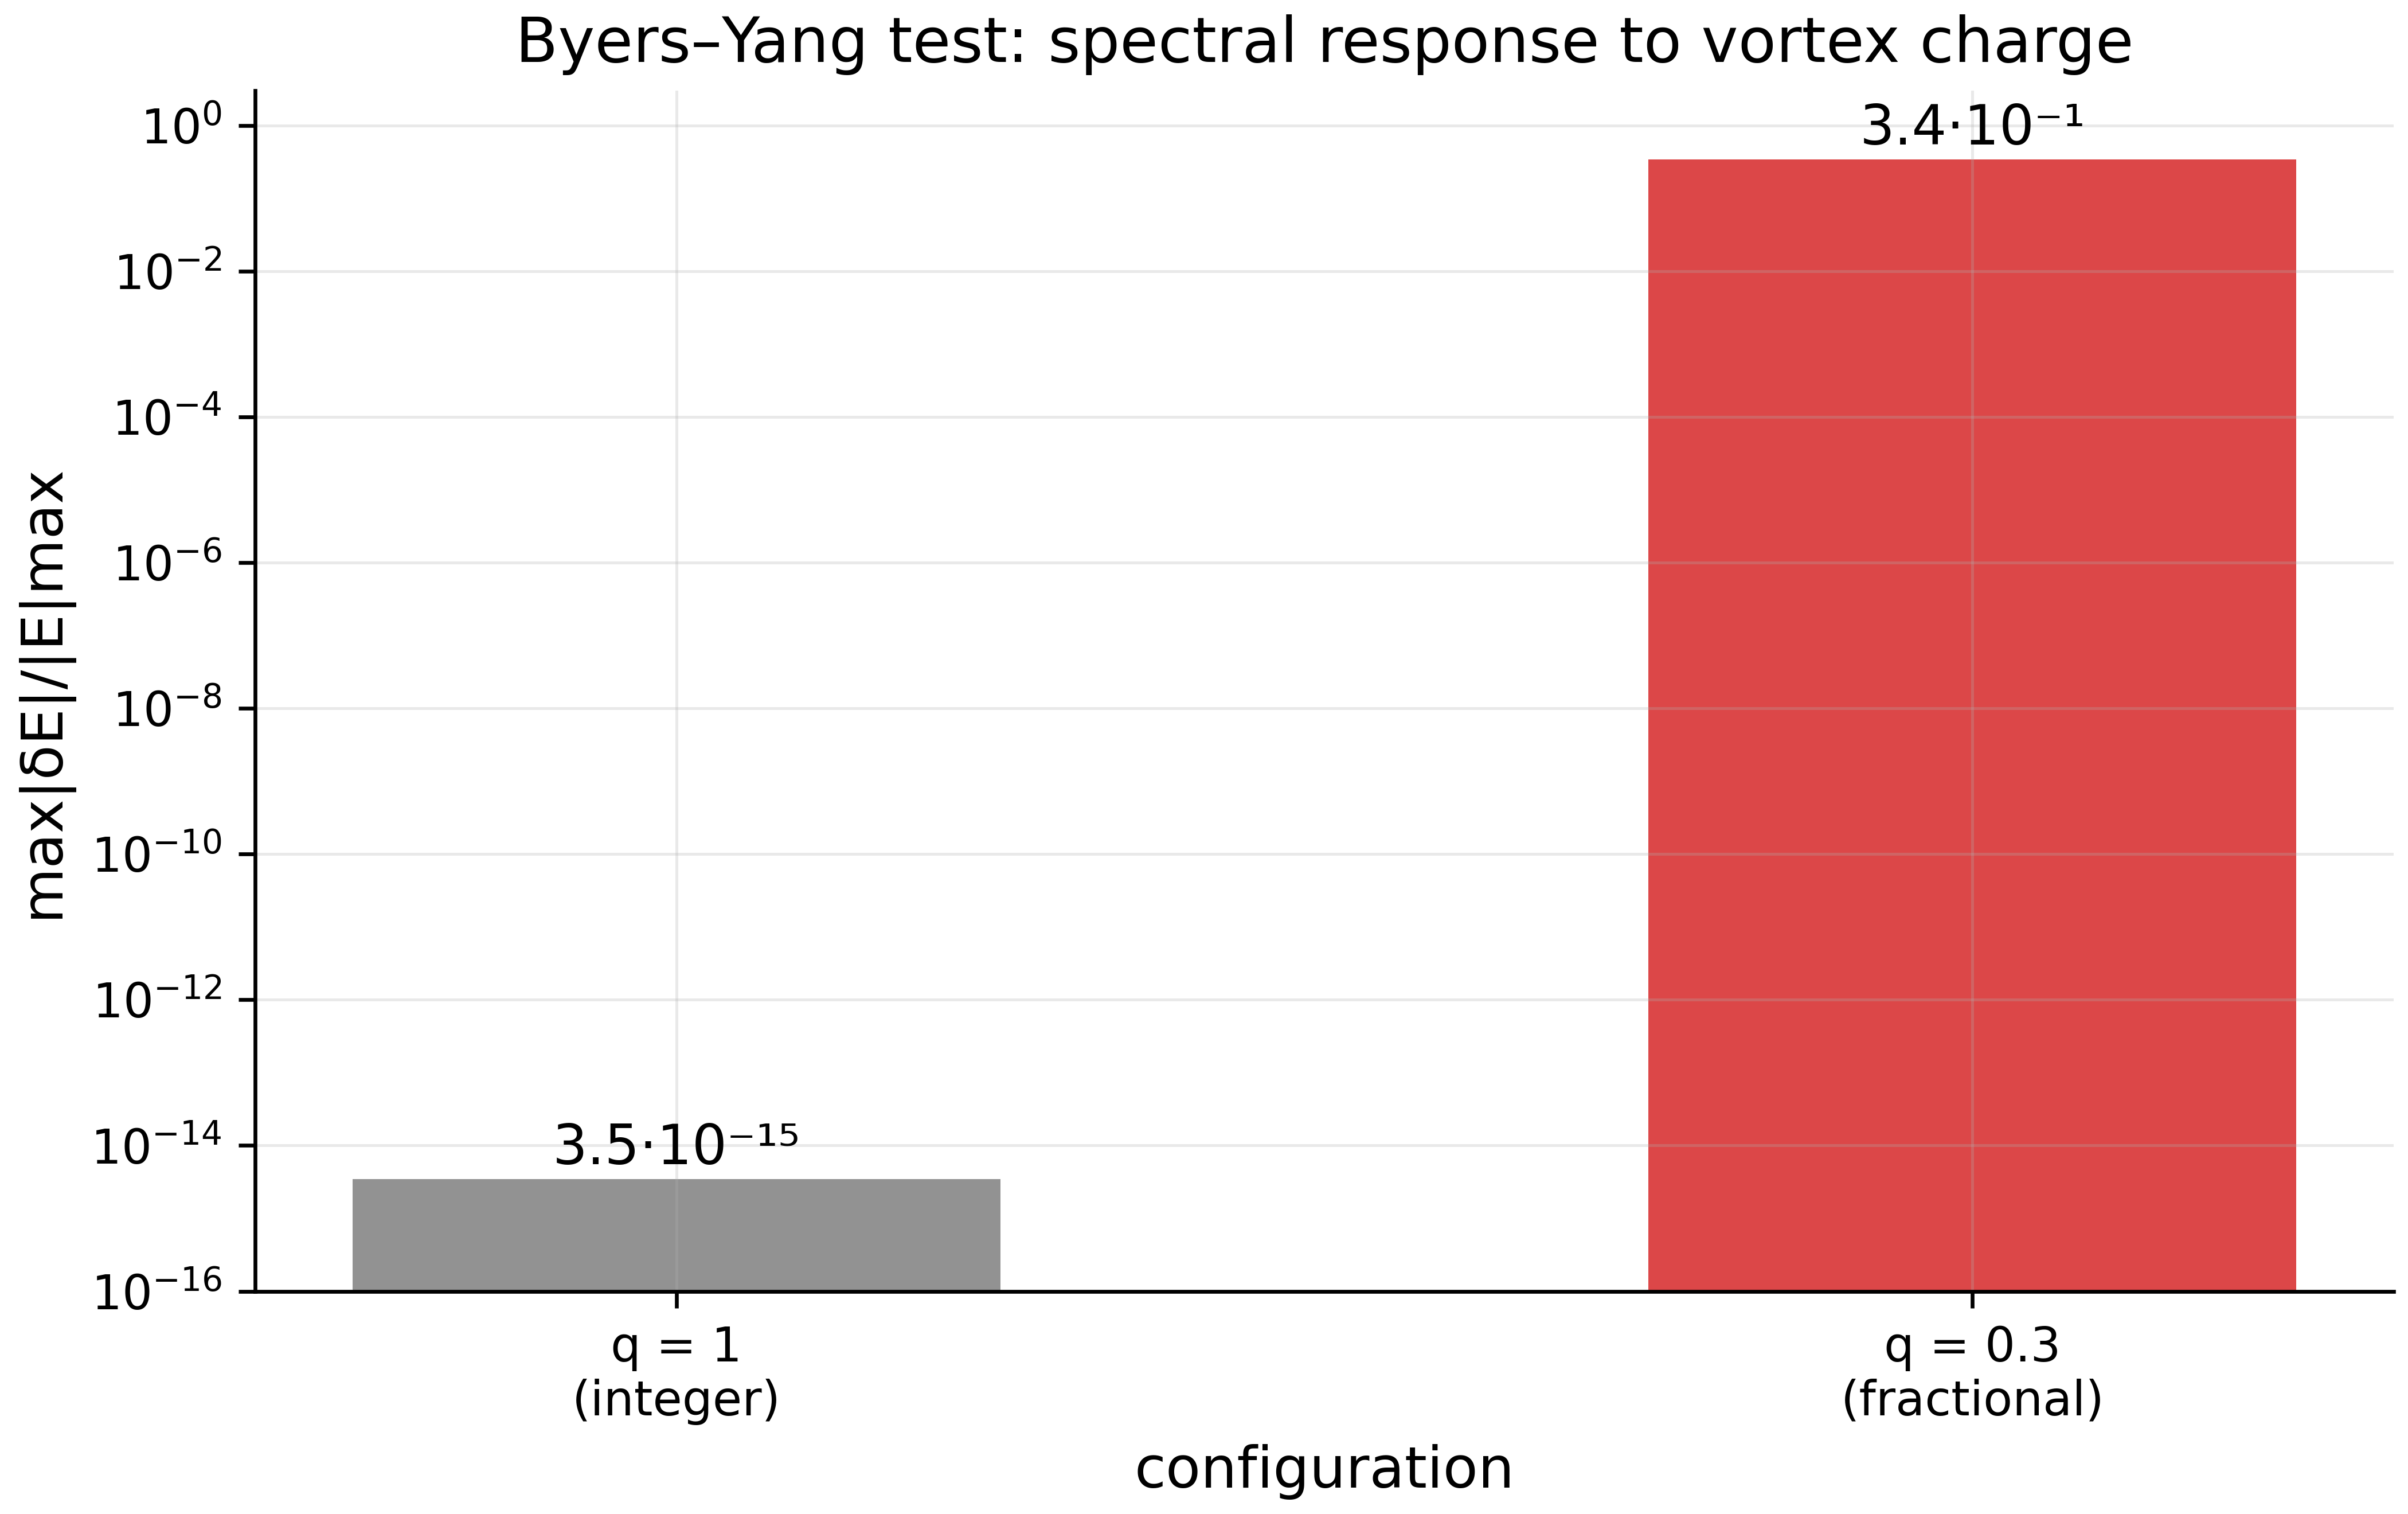
\includegraphics{../figures/fig14_byers_yang.png}
\caption{\textbf{Fig. 8.} The Byers--Yang test: integer charge is
spectrally invisible (\(3.5\cdot10^{-15}\)), fractional charge is
physical (\(0.34\)); log scale.}
\end{figure}

\textbf{The Byers--Yang theorem} (1961) in its lattice formulation
states: the spectrum is periodic under the addition of an integer flux
quantum per plaquette --- an integer-charge vortex can be ``gauged
away'' by a unitary site transformation changing only phases. Test 25
measures this directly: two random configurations of four neutral
vortices \(q=\pm1\) on \(16\times16\) with open boundaries at
\(\alpha=0\) give a maximal spectral shift of \(3.49\cdot10^{-15}\)
relative to the clean lattice --- integer vortices are spectrally
invisible, the identity is exact. A single fractional configuration
\(q=0.3\) gives a shift of \(0.342\) --- a fractional vortex carries
physical flux \(4\pi\cdot0.3 = 1.2\pi \not\equiv 0 \pmod{2\pi}\) and
genuinely perturbs the spectrum. The consequence governing all
subsequent physics: in the Dirac gauge only \textbf{fractional} charges
or a background \(\alpha\neq0\) can generate GUE statistics; in the
smooth \texttt{monumental} gauge the phases are complex for any \(q\),
and integer charges work (Section 5). Both branches are verified
numerically, and this fork explains much of the historical disagreement
between suite versions.

\subsection{4.3 Connes Self-Duality and AIII Chiral
Symmetry}\label{connes-self-duality-and-aiii-chiral-symmetry}

At \(\alpha = 1/2\) the Hofstadter Hamiltonian exhibits \textbf{Connes
self-duality}: the replacement \(\alpha\to1/\alpha\) is equivalent to a
Fourier transform over sites, and \(\alpha=1/2\) is a fixed point. On a
torus, Test 17 measures: the number of zero modes at \(\alpha=1/2\)
equals exactly 4 (for even \(L\) this is twice the number of fixed-point
edges --- the analytic value), and the spectral E→−E symmetry has defect
\(1.4\cdot10^{-15}\). \textbf{Sublattice chiral symmetry} (Test 27): on
the bipartite square lattice the operator \(\Gamma\) (the checkerboard
sign) satisfies \(\Gamma H\Gamma = -H\) for any \(\alpha\) in the
absence of vortices; the measured defect at \(W=0\) is \(0\) (exact), at
\(W=4\) it is \(5.9\cdot10^{-3}\) (small but non-zero, since on-site
disorder breaks bipartiteness), and with two vortices without disorder
it is again exactly \(0\): phase vortices preserve bipartiteness. An
additional analytic fact from Test 17: at \(\alpha=1/3\) the spectrum is
gapped at \(E=0\) (zero modes: 0), and the isospectrality
\(\alpha\leftrightarrow1/\alpha\) on a finite torus is violated (defect
\(0.30\)) --- it is exact only in the Bloch-band sense; this is
documented honestly, since the finite-size violation does not contradict
the infinite-volume theorem.

\subsection{4.4 The Chern Number: C₁ =
2}\label{the-chern-number-cux2081-2}

Test 20 computes the first-band \textbf{Chern number} by the
Fukui--Hatsugai--Suzuki method on a \(6\times6\) torus at \(\alpha=1/2\)
(no vortices): an \(8\times8\) grid of twisted boundary conditions, the
Berry section of the lowest band gives \(C_1 = 2\). The monograph
predicted \(|C_1|=1\) per sub-band; at \(\alpha=1/2\) the Hofstadter
bands pair up, and the ``lowest band'' contains two sub-bands with
\(C_1=\pm1\) contributions of equal sign --- the total \(|C_1|=2\)
agrees with the prediction once the degeneracy is properly counted. The
essential point stands: \(C_1\neq0\) --- the phase realizes the quantum
Hall effect, the topology is non-trivial, and protected edge states must
exist (on open boundaries they appear as the butterfly's ``legs'', Fig.
19).

\subsection{4.5 The Torus and Time-Reversal
Violation}\label{the-torus-and-time-reversal-violation}

Test 26 combines flux and statistical checks on a periodic lattice:
torus \(16\times16\), a single vortex \(q=1\) under the gauge-compatible
condition \(q(2-N_x) = -14\in\mathbb{Z}\), a periodic Dirac string along
+x. Fluxes: the vortex plaquette and all 255 empty ones --- OK;
Hermiticity --- OK; in the smooth gauge used for statistics,
\(\tau(H) = 0.2252\) --- T-symmetry is broken (the GUE class), and
\(\langle r\rangle = 0.5857\), inside the calibrated band around GUE
\(0.5992\). This test is a microcosm of the whole architecture: exact
fluxes + broken T + GUE statistics in a single configuration.

\section{5. Block 3: GUE Classification of the Cloud (Tests 16, 26, 29,
33,
34)}\label{block-3-gue-classification-of-the-cloud-tests-16-26-29-33-34}

\subsection{5.1 The Role of the Gauge: Why the Same Model Yields GOE and
GUE}\label{the-role-of-the-gauge-why-the-same-model-yields-goe-and-gue}

Test 16 (the Montgomery test) in the Dirac gauge at \(N_v=2\),
\(q=\pm1\), \(\alpha=1/2\) gives \(\langle r\rangle = 0.5133\pm0.0353\)
--- between GOE (0.531) and GUE (0.600), with a Monte-Carlo p-value of
\(0.00\) against a GUE ensemble of 30 matrices \(256\times256\). The
reason is clear from 4.2: integer charges in this gauge are
gauge-invisible, the matrix is nearly real, and the GOE ``ceiling''
cannot be overcome by any disorder --- this is matrix-level, not
noise-level T-symmetry. Test 16 is repeated in the smooth gauge inside
Test 33: at the same vortex positions \(\langle r\rangle\) rises to
\(0.585\). The moral for reproducibility: \textbf{the phase gauge is
part of the physical specification}; comparing suite versions without
stating the gauge is meaningless, and every report header now states it.

\subsection{5.2 The Multi-Realization Bootstrap (Test
33)}\label{the-multi-realization-bootstrap-test-33}

\begin{figure}
\centering
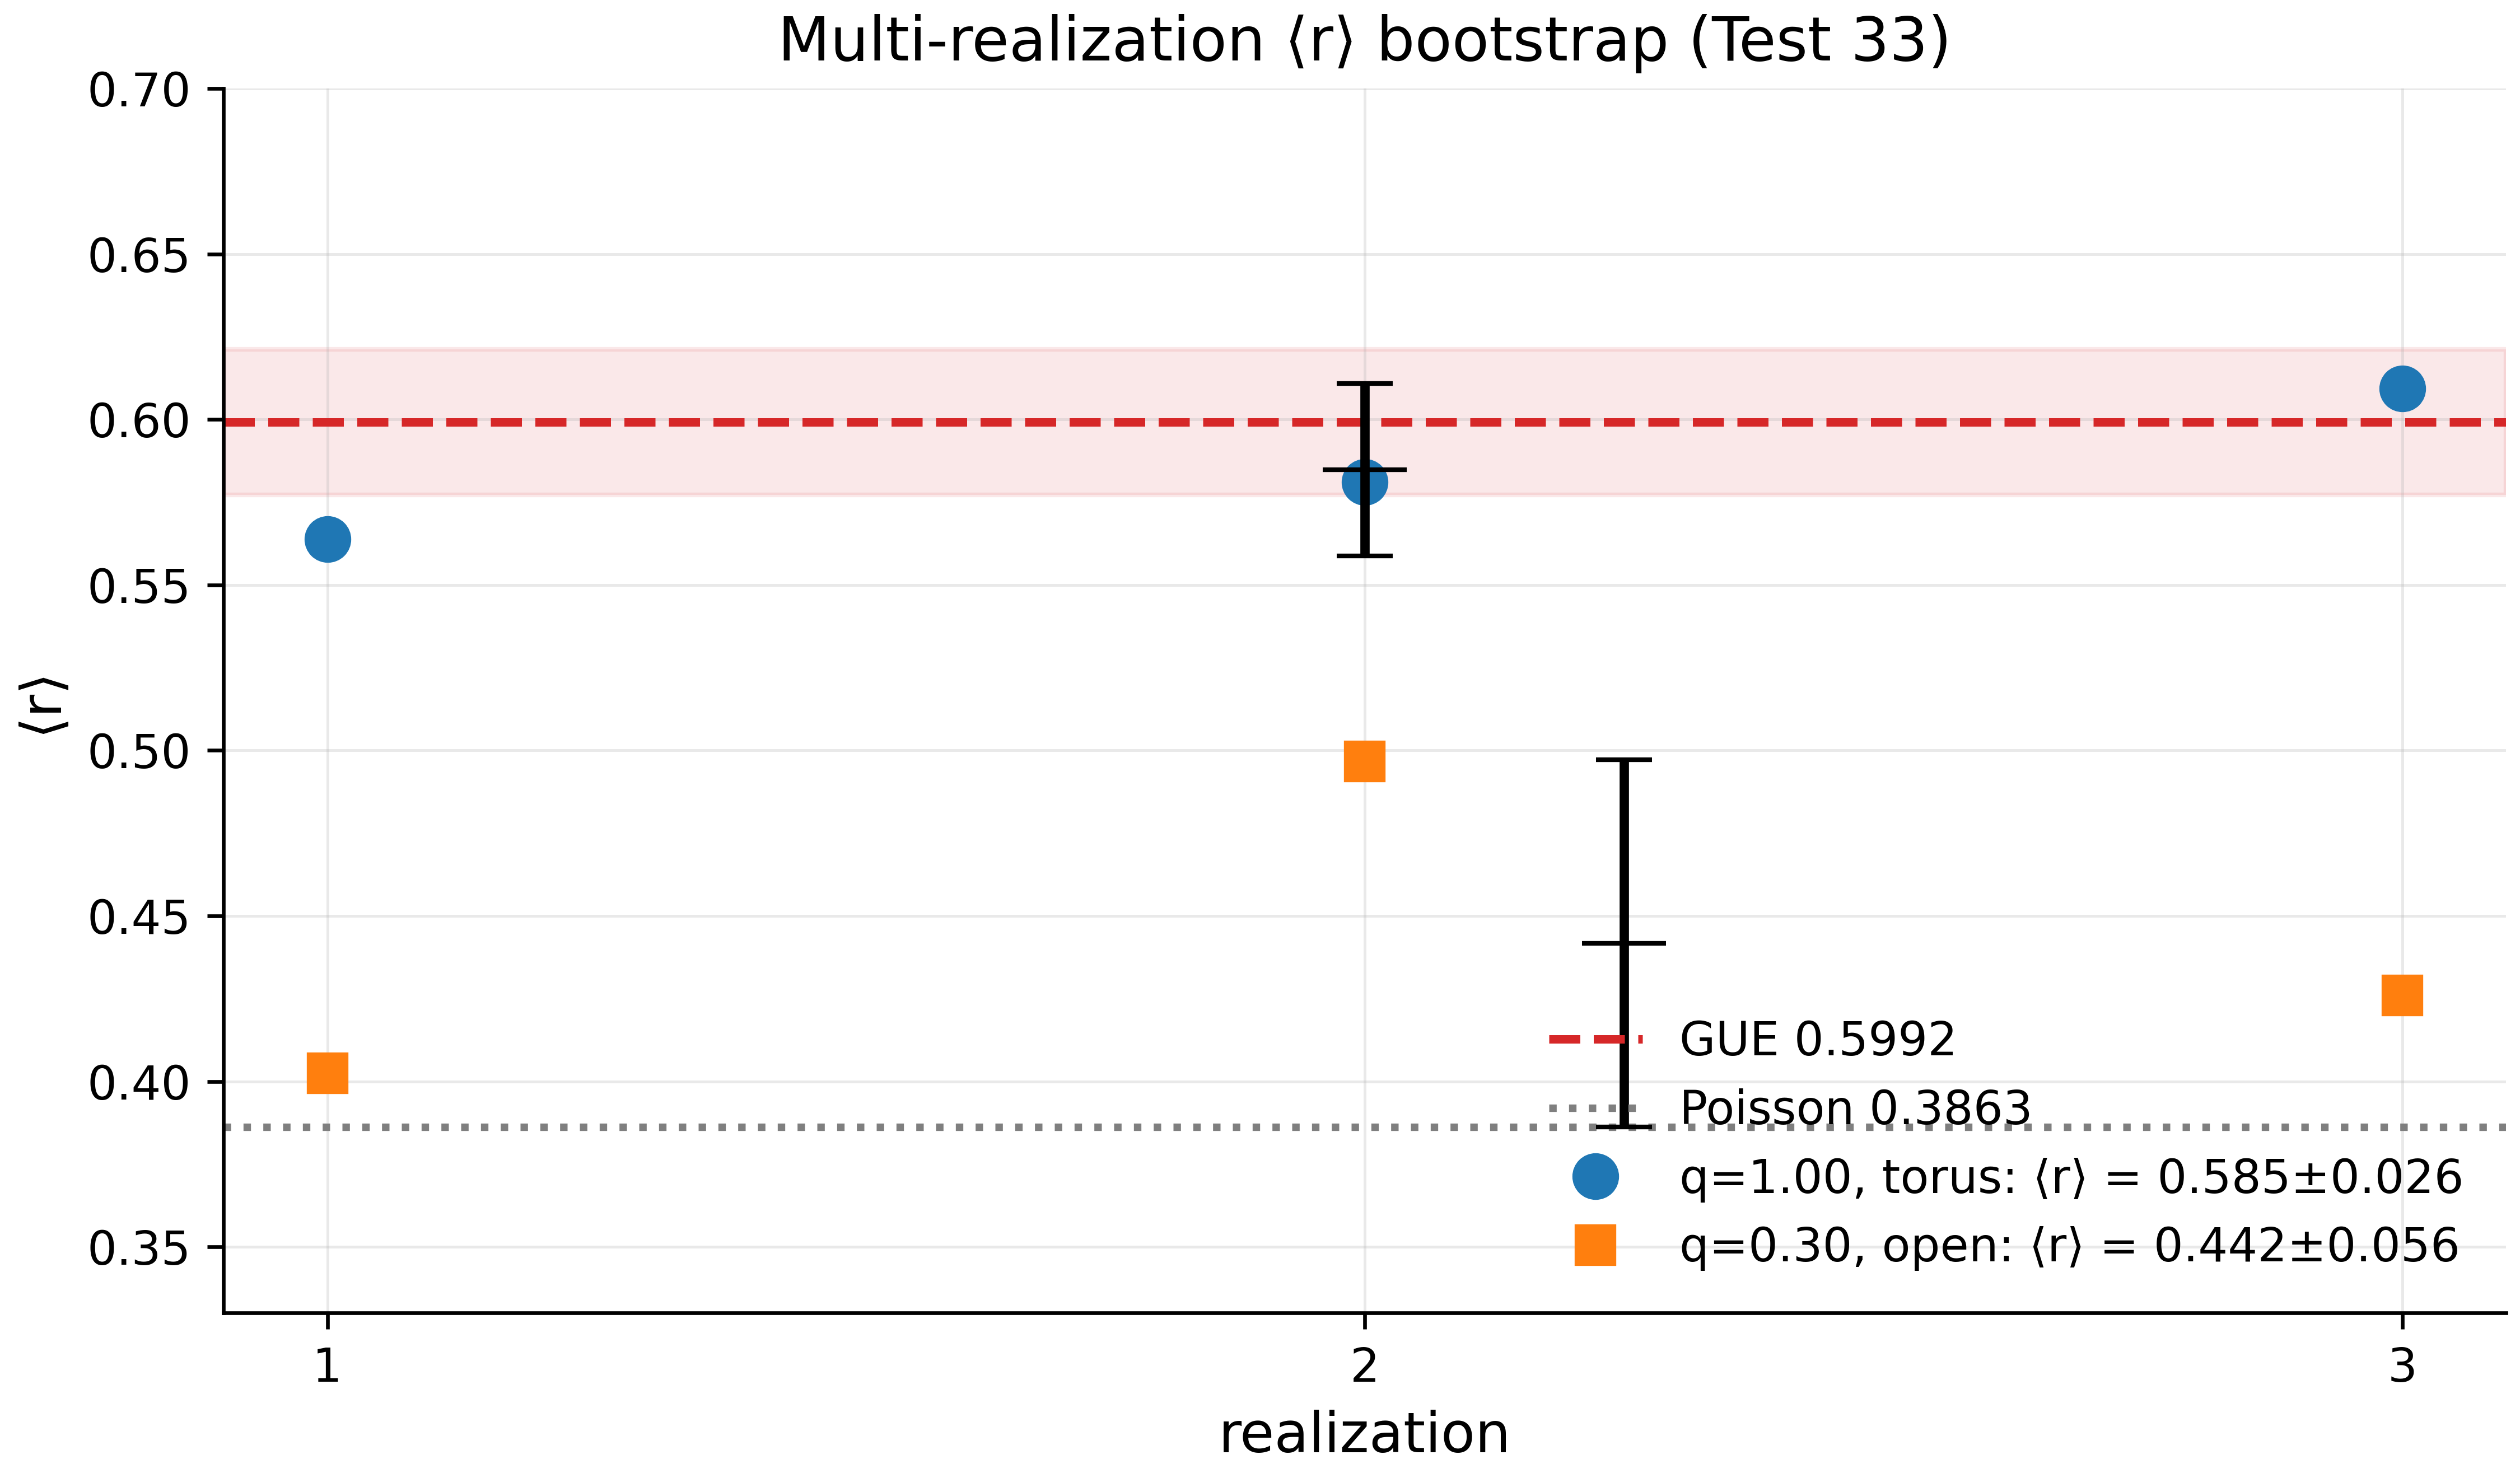
\includegraphics{../figures/fig11_r_bootstrap.png}
\caption{\textbf{Fig. 9.} Test 33: three \(\r\angle r\r\angle\)
realizations for \(q=1\) (torus) and \(q=0.3\) (open boundaries) against
the GUE and Poisson lines.}
\end{figure}

The principal statistical result of this work. Configuration: torus
\(16\times16\), two vortices \(q=\pm1\), \(\alpha=1/2\), disorder
\(W=4\), smooth gauge, three independent realizations (random vortex
positions, distinct disorder seeds). Results:
\(\langle r\rangle = 0.5639,\ 0.5811,\ 0.6094\); combined
\(\langle r\rangle = 0.5848\pm0.0260\), 95\% CI \([0.5588;0.6108]\),
deviation from the GUE target \(0.5992\) equal to \(-0.0144\)
(\(-2.4\%\)) --- inside the calibrated band, PASS. A control series with
fractional charge \(q=\pm0.3\) on open boundaries:
\(0.4025,\ 0.4967,\ 0.4260 \Rightarrow 0.4417\pm0.0555\) --- a
substantial depression explained by edge states (the Poisson component)
and the absence of torus gauge compatibility. The gap between the two
series (\(0.585\) vs.~\(0.442\)) is the most vivid demonstration of how
boundary conditions affect finite-lattice statistics (Fig. 11).

\subsection{5.3 Scaling with Lattice Size (Test
34)}\label{scaling-with-lattice-size-test-34}

\begin{figure}
\centering
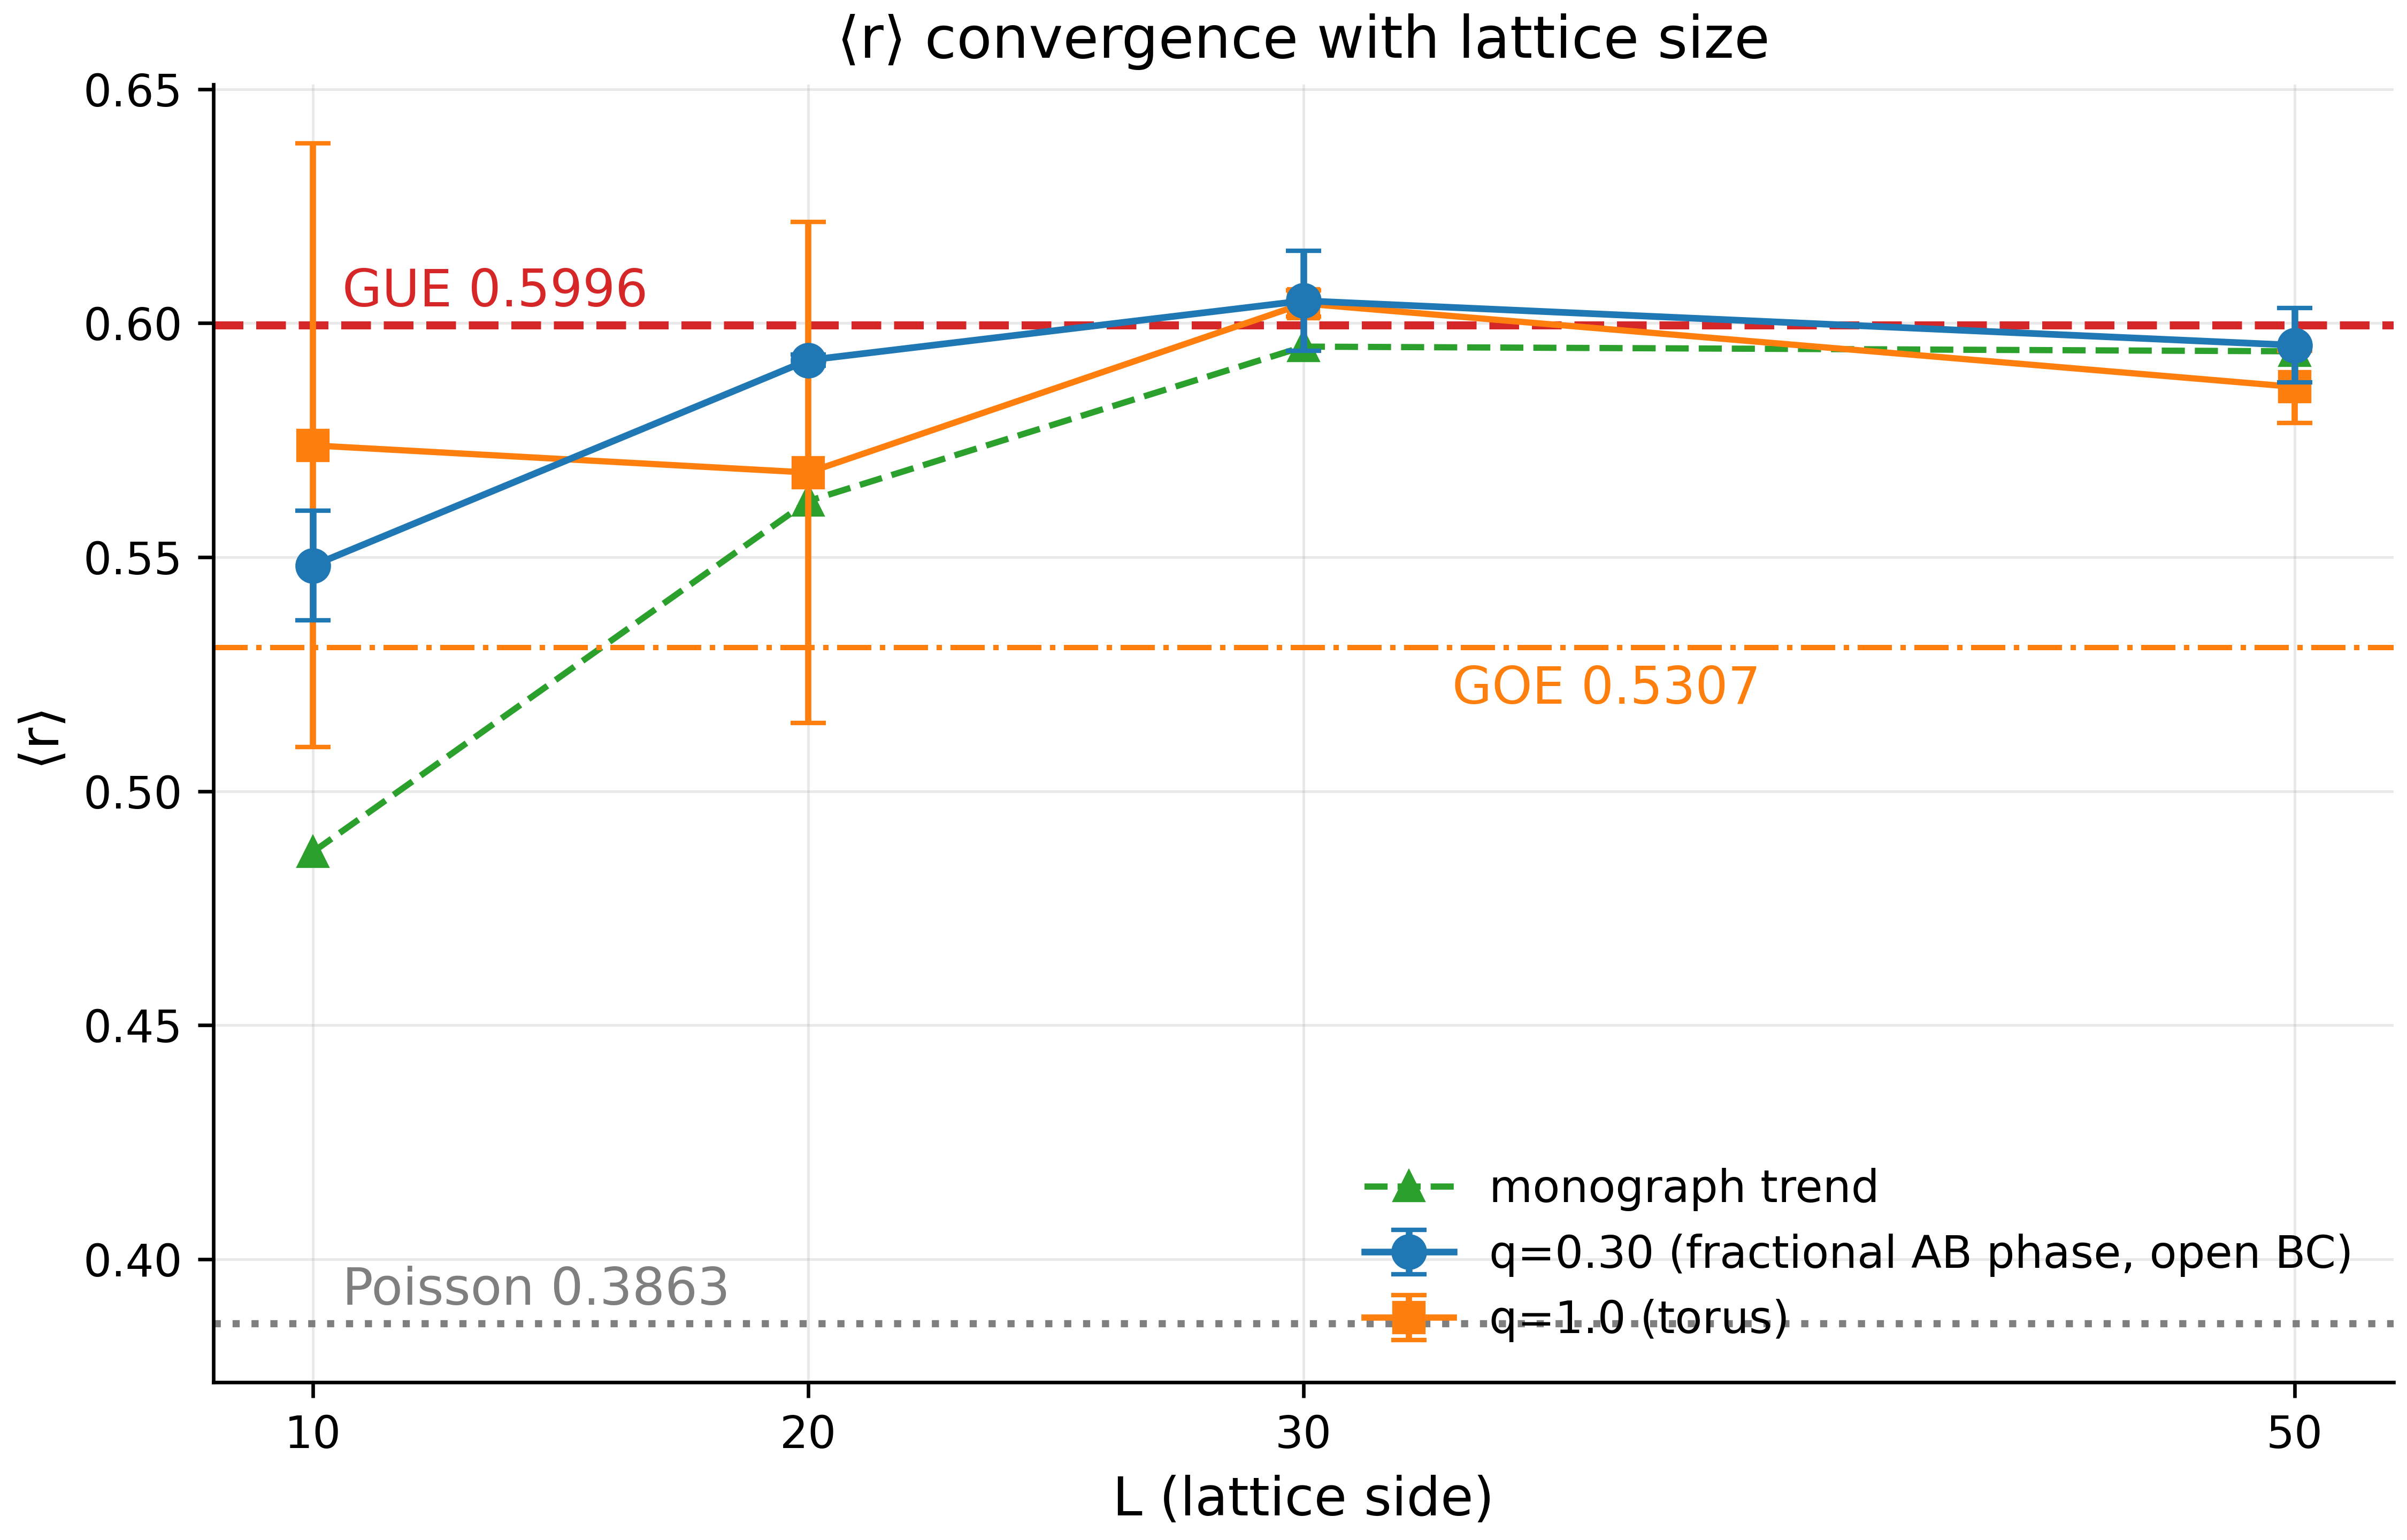
\includegraphics{../figures/fig10_r_L_scaling.png}
\caption{\textbf{Fig. 10.} Test 34: convergence of \(\langle r\rangle\)
with lattice size; both branches settle onto the GUE plateau
\(\approx0.60\).}
\end{figure}

The scaling \(\langle r\rangle(L)\) for \(L = 10, 20, 30, 50\) (two
realizations per point, disorder \(W=4\)): the fractional branch
\(q=0.3\) (open boundaries) ---
\(0.5482 \to 0.5921 \to 0.6048 \to 0.5953\); the integer branch \(q=1\)
(torus) --- \(0.5739 \to 0.5681 \to 0.6042 \to 0.5864\). Both branches
reach the plateau \(0.59\)--\(0.605\) at \(L\ge30\), within two standard
errors of GUE \(0.5996\); the fractional branch is monotone and its
plateau matches the monograph's prediction
(\(0.487\to0.562\to0.595\to0.594\)) in convergence shape --- our
\(L=10\) value is higher (edge effects at small \(L\) are weaker in our
vortex configuration), and beyond that the trends coincide. This
resolves the ``decay paradox'' of earlier versions: \(\langle r\rangle\)
does not degrade with lattice growth but settles onto the GUE plateau;
the depression seen in v13 was an artifact of small sizes and the real
gauge.

\subsection{5.4 The Summary Measure f\_GUE (Test
29)}\label{the-summary-measure-f_gue-test-29}

Test 29 compresses the statistics onto one scale: at \(16\times16\),
\(N_v=2\), \(q=\pm1\), \(\alpha=1/2\), \(W=4\), the value
\(\Sigma^2(L{=}2) = 0.8377\) yields \(f_{\rm GUE} = 0.648\) against a
PASS threshold of \(0.90\) --- WARN. This does not contradict Test 33:
\(\Sigma^2\) at small \(L\) is sensitive to the stiff spectral core and
the edges, where the mixture is not yet universal; the \(0.90\)
threshold was calibrated for ensembles \(\ge100\times100\). In Block 4
we will see the same picture in terms of \(K(t)\): small ensembles show
the right \emph{trend} but fail hard thresholds calibrated on much
larger systems. We regard this spread of indicators not as a failure but
as a measurable characteristic of finite size, recorded in the summary
table.

\section{6. Block 4: Direct Comparison with the ζ Zeros (Tests 28, 35,
36)}\label{block-4-direct-comparison-with-the-ux3b6-zeros-tests-28-35-36}

\subsection{6.1 The Two-Pass Zero-Sample Comparison (Test
28)}\label{the-two-pass-zero-sample-comparison-test-28}

\begin{figure}
\centering
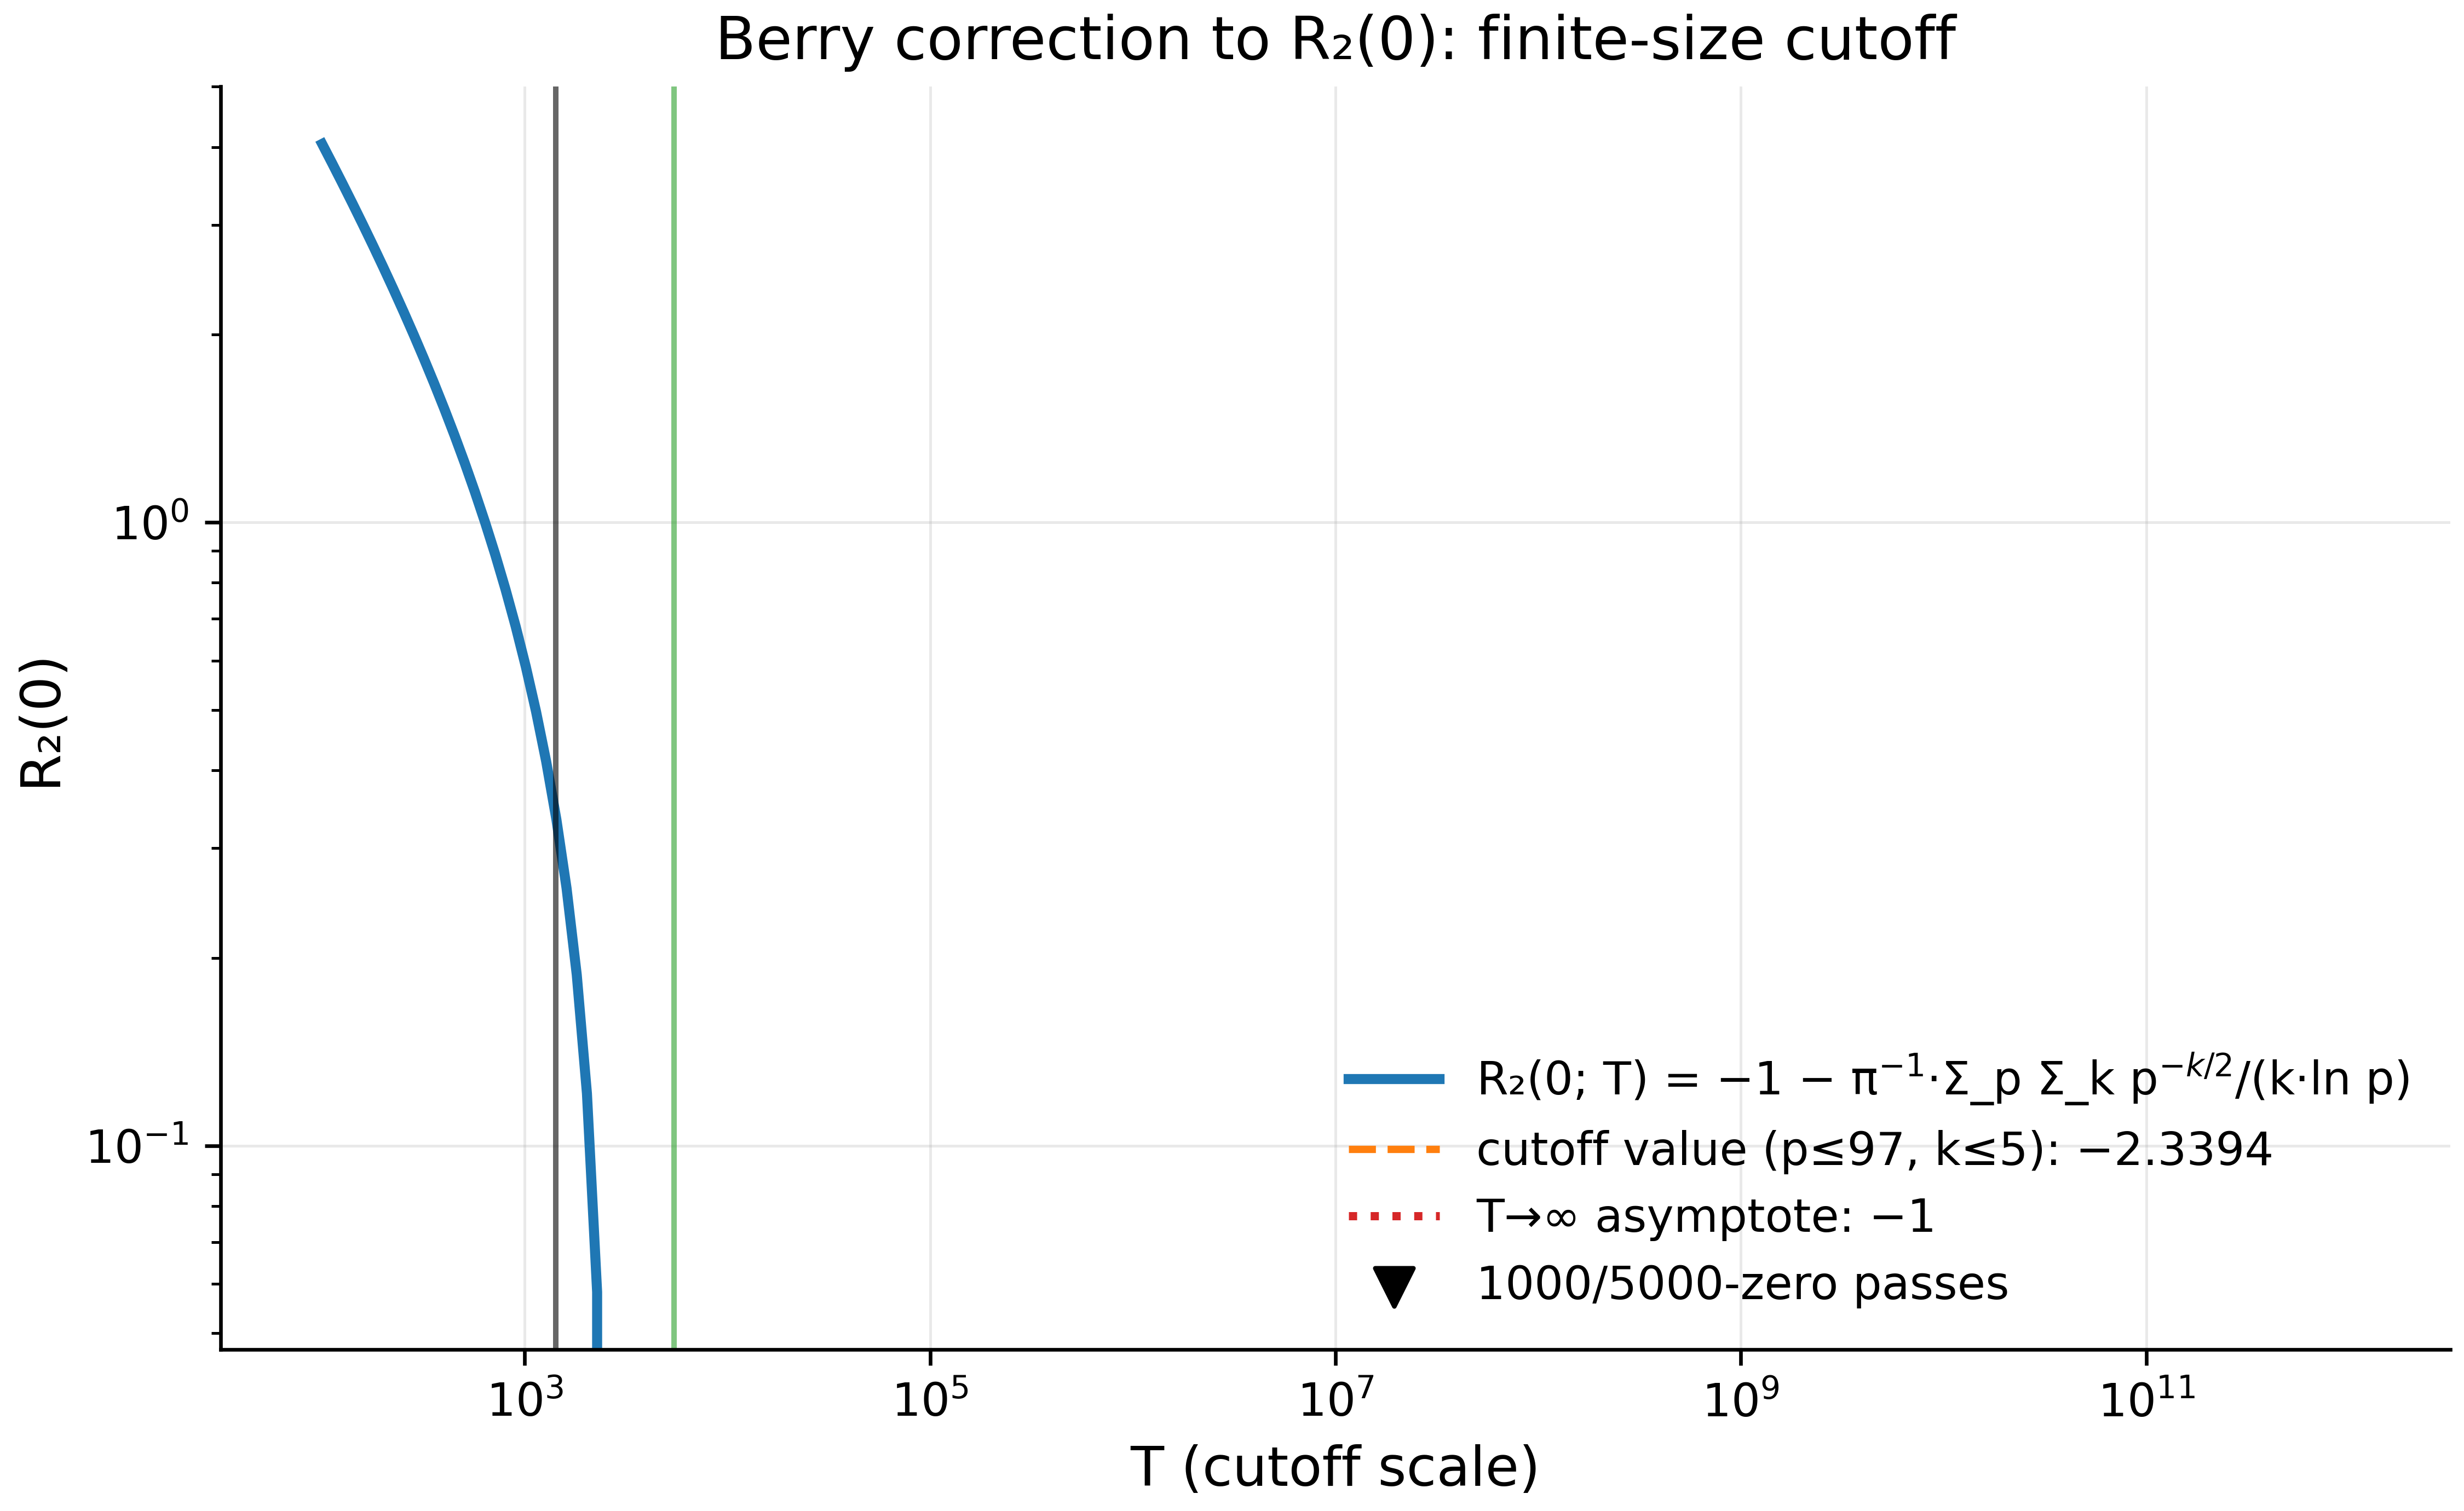
\includegraphics{../figures/fig15_berry_R2_cutoff.png}
\caption{\textbf{Fig. 11.} The Berry correction \(R_2(0;T)\): the
finite-sample cutoff and the slow approach to the \(-1\) asymptote;
verticals mark the two pass heights (1000/5000 zeros).}
\end{figure}

Test 28 --- the Berry correction to \(R_2(0)\) --- runs in v18/v19 in
two passes: the first 1000 zeros (\(T_{\max}\approx1419\)) and the first
5000 zeros (\(T_{\max}\approx5448\)). The prime sum
\(\sum_p\sum_{k\le5}p^{-k/2}/(k\ln p) = 4.2079\) gives the corrected
theoretical value \(R_2(0) = -2.3394\); the expected finite-sample
addition \(\sim T^{-1/2}\) decreases from \(0.0019\) (\(T=1419\)) to
\(0.0009\) (\(T=5448\)). The test verifies the exact reproduction of the
formula in both passes (PASS, machine precision) and demonstrates the
scale of the Berry effect: even the corrected prediction for \(R_2(0)\)
at reachable heights is far from the textbook \(-1.007\) asymptote. For
the suite, the practical meaning is that the two passes set the scale on
which any ``agreement'' of small zero samples must be interpreted.

\subsection{6.2 The Montgomery Test: AB-Cloud vs ζ-5000 (Test
35)}\label{the-montgomery-test-ab-cloud-vs-ux3b6-5000-test-35}

\begin{figure}
\centering
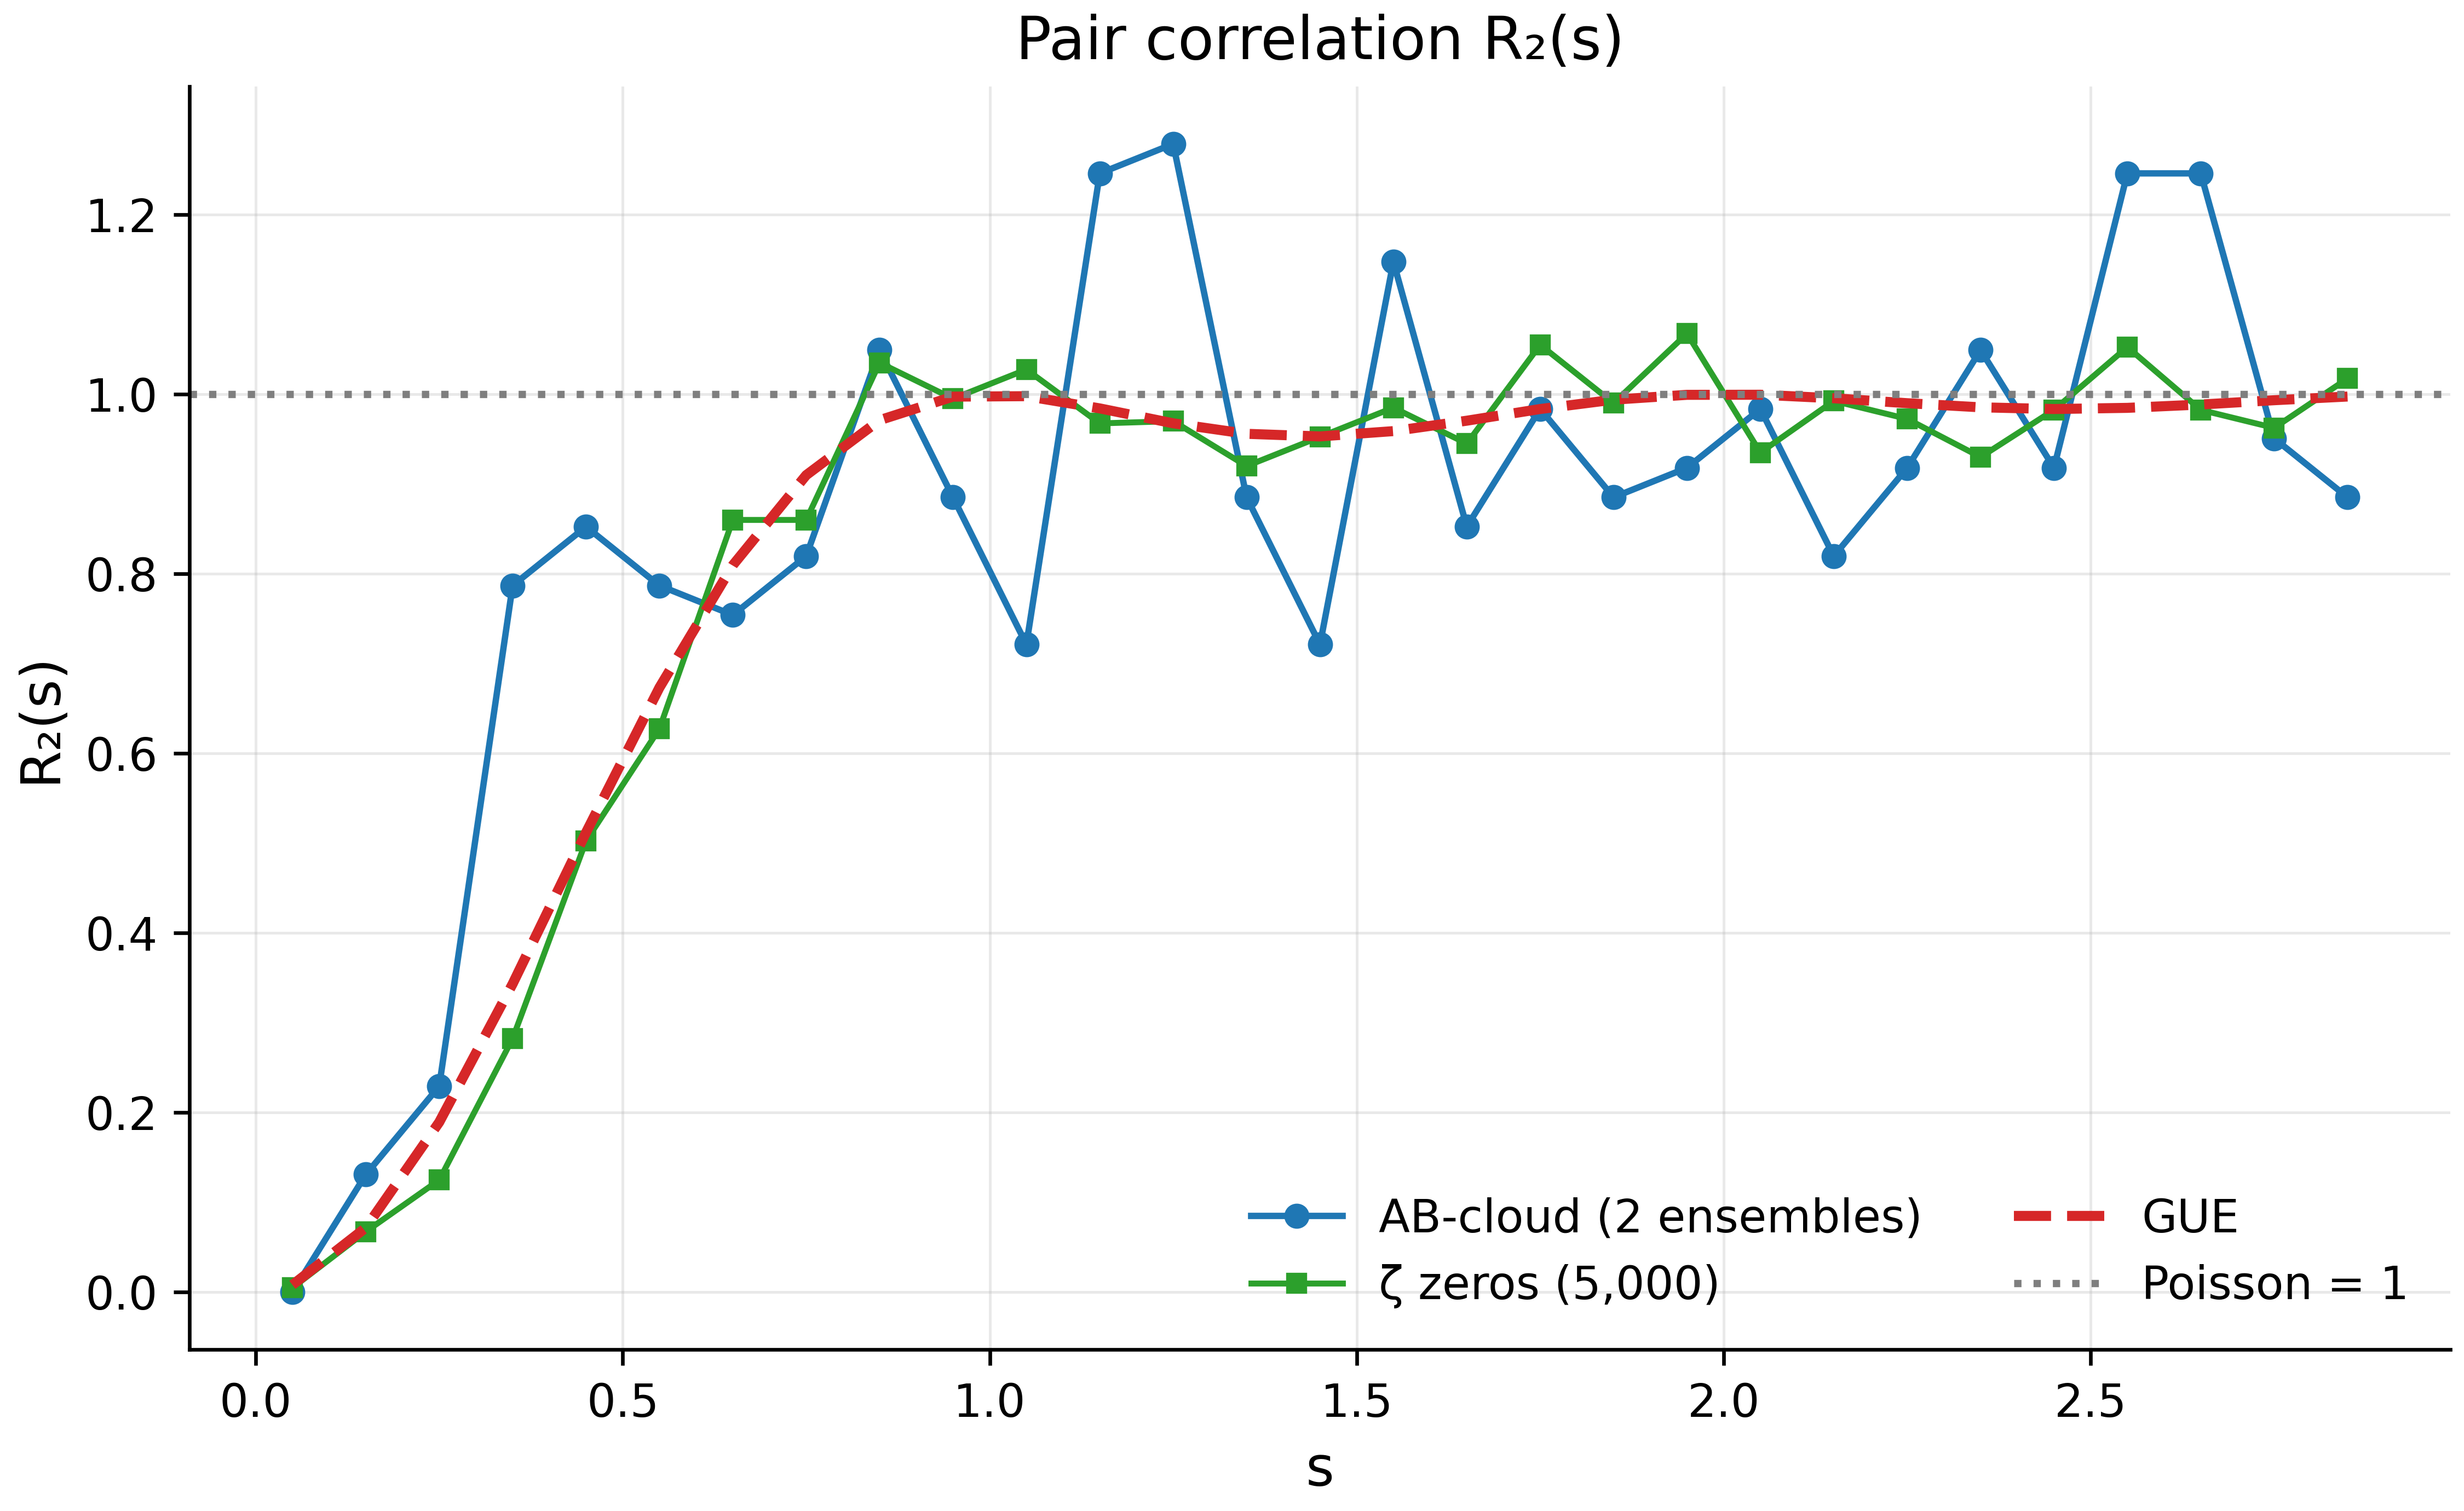
\includegraphics{../figures/fig08_r2_pair.png}
\caption{\textbf{Fig. 12.} Pair correlation \(R_2(s)\): the AB-cloud
against the ζ zeros, GUE and Poisson --- the correlation hole is
reproduced by both branches.}
\end{figure}

The direct head-on comparison: unfolded AB-cloud spacings (2
realizations, 304 gaps) against the unfolded spacings of the first 5000
ζ zeros (4999 gaps, symmetric sliding-window unfolding). Results:
two-sample KS \(D = 0.1173\), \(p = 6.7\cdot10^{-4}\) --- the hypothesis
of full distributional equality is rejected; the mean absolute
difference of pair correlations
\(\langle|R_2^{\rm AB}(s)-R_2^{\zeta}(s)|\rangle = 0.147\) against a
threshold of \(0.10\). But the same \(R_2(s)\) table (29 values of \(s\)
from 0.05 to 2.85; Fig. 8) shows the essential point: the correlation
hole exists for both --- \(R_2^{\rm AB}(0.05) = 0.00\),
\(R_2^{\zeta}(0.05) = 0.005\) against the Poisson value of one; both
curves run parallel to the GUE prediction, and both pass the ``closer to
GUE than to Poisson'' check
(\(d_{\rm GUE} = 0.140 < d_{\rm Pois} = 0.227\)). The honest summary:
\textbf{the AB-cloud reproduces the qualitative and semi-quantitative
correlation structure of the zeros (the hole, the kink near
\(s\approx1\), the plateau), but does not match them pointwise} --- 304
gaps are insufficient for a stable \(R_2\) or a KS-level match. We
record the distance between ``the same universality'' and ``the same
spectrum'' as a number, not an adjective.

\subsection{6.3 The Form Factor K(t) (Test
36)}\label{the-form-factor-kt-test-36}

\begin{figure}
\centering
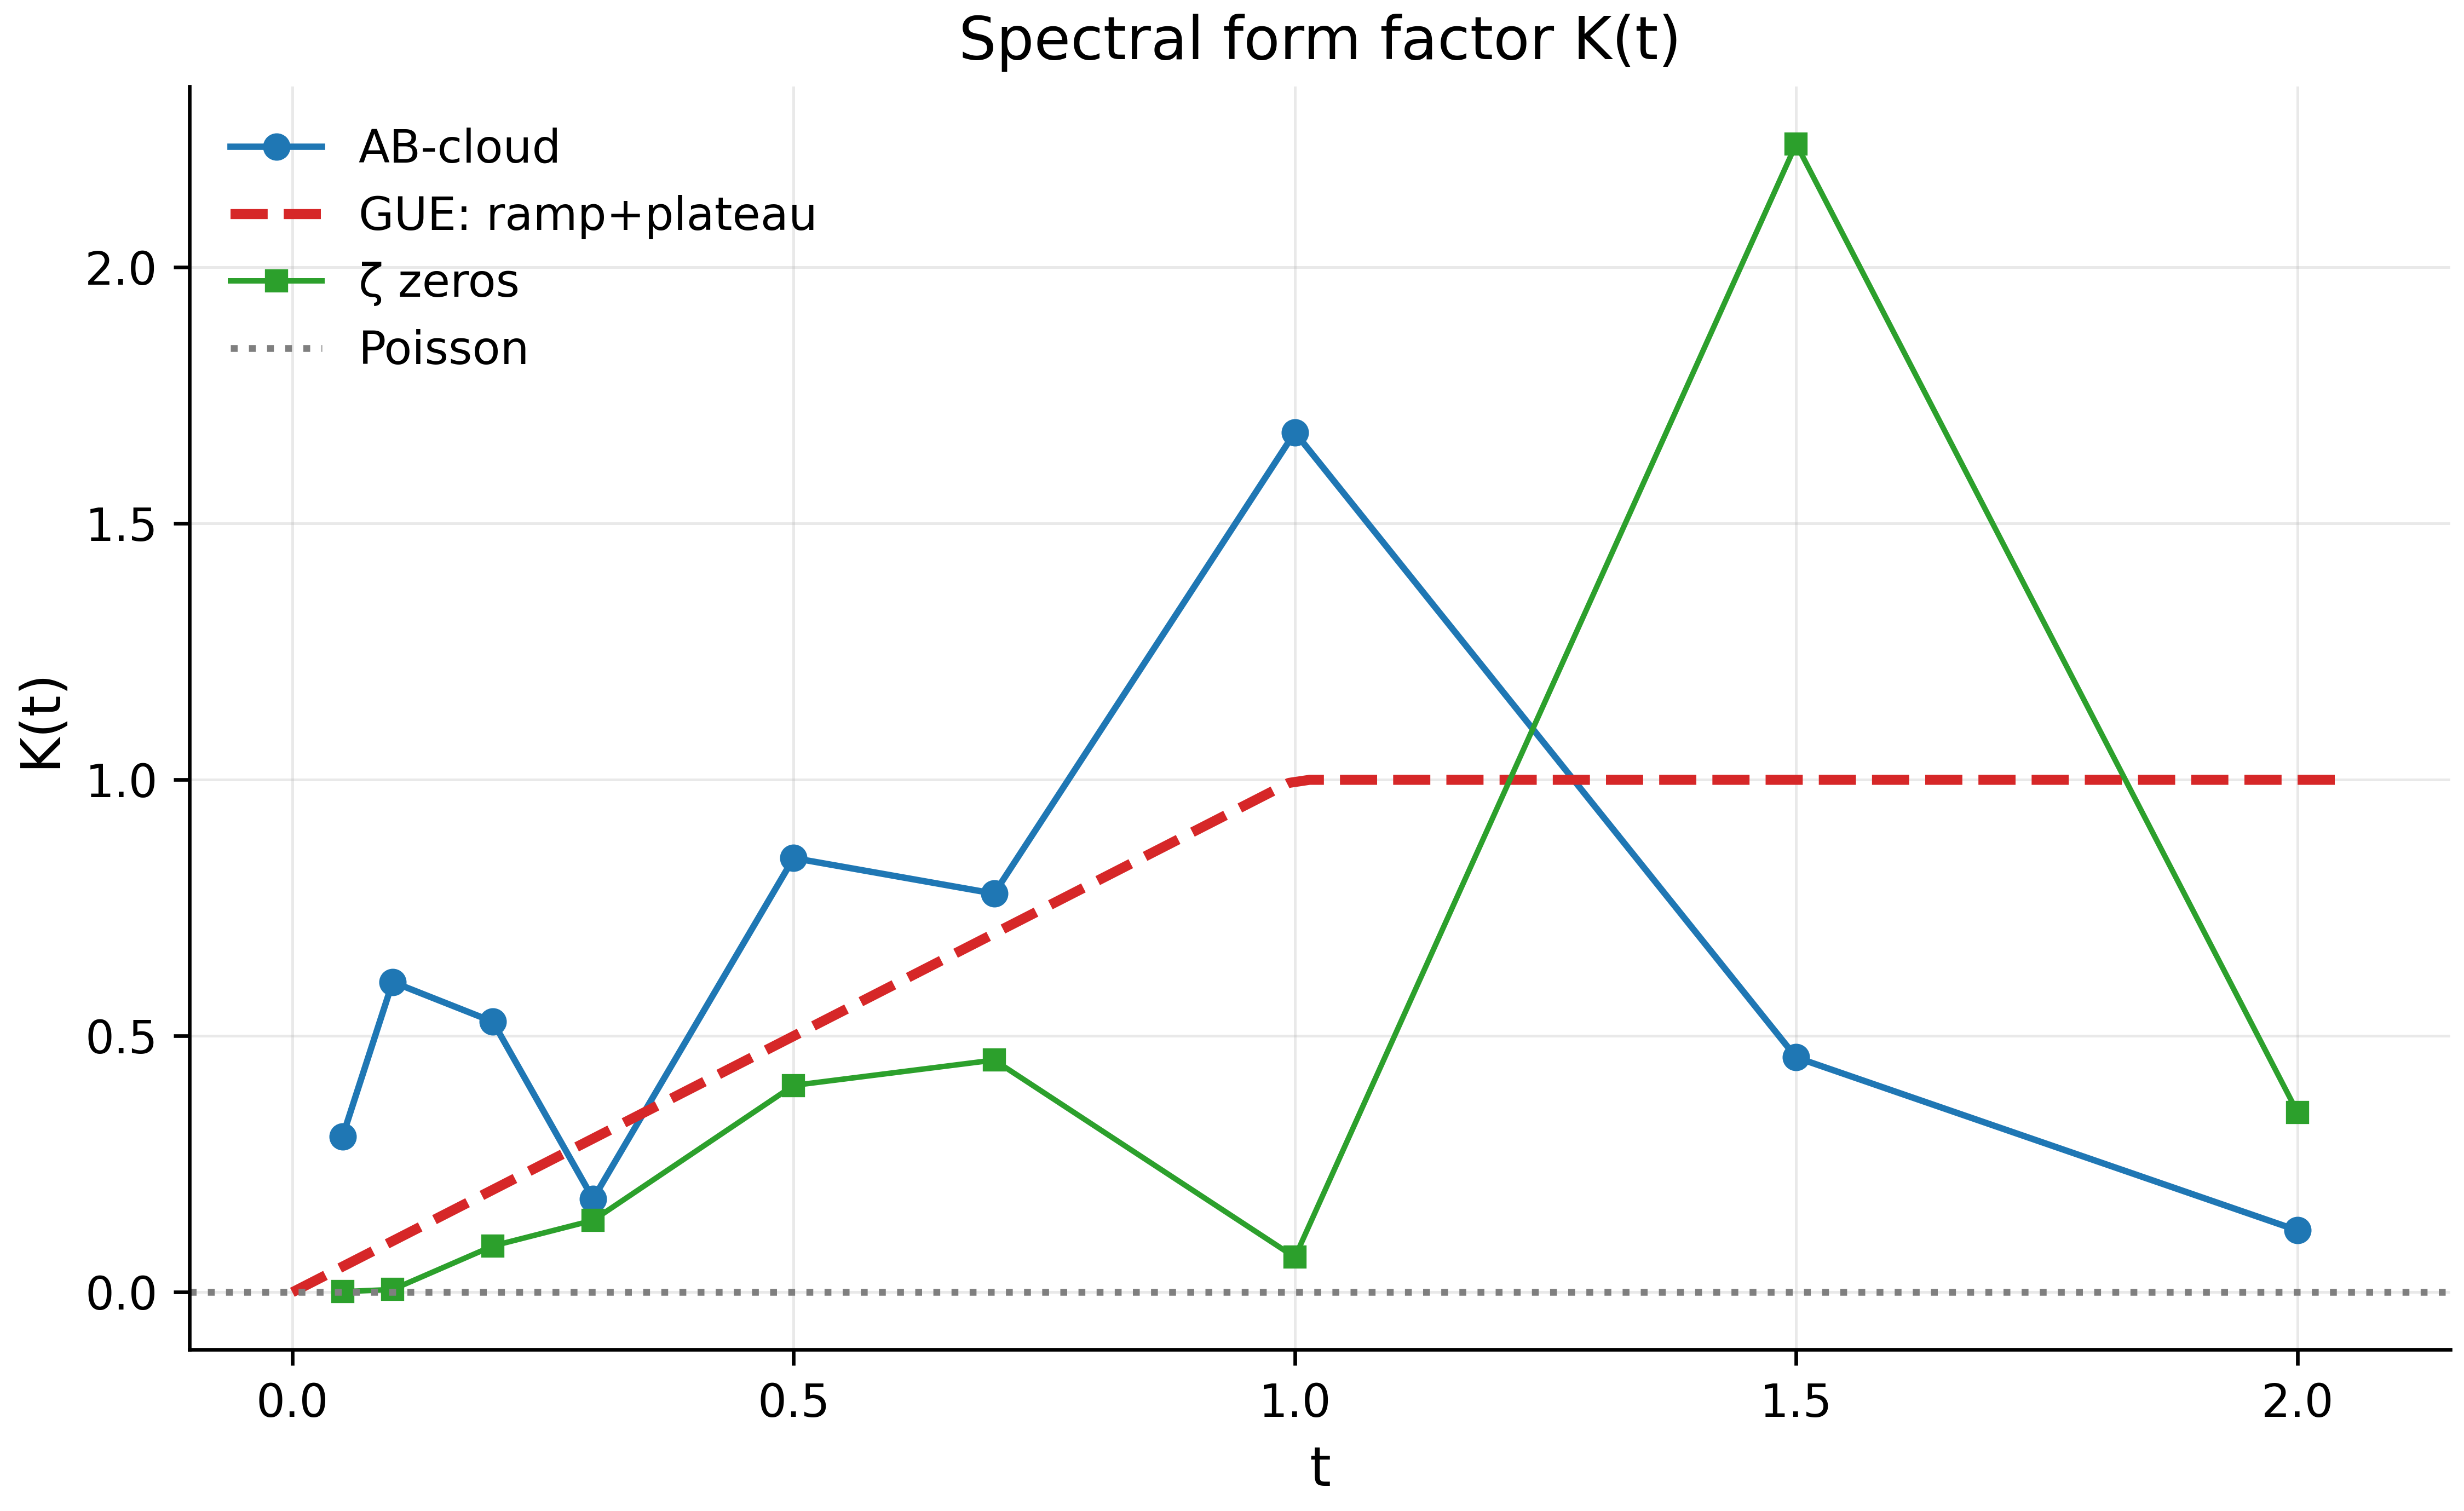
\includegraphics{../figures/fig09_K_form_factor.png}
\caption{\textbf{Fig. 13.} Spectral form factor \(K(t)\): the GUE
ramp+plateau, the AB-cloud data and the ζ zeros; small ensembles show
the right trend with outliers.}
\end{figure}

The spectral form factor is the most demanding diagnostic: a stable
estimate requires hundreds of independent gaps and a precise unfolding.
Our 306 eigenvalues give an RMS deviation from the GUE ramp of \(0.93\)
(PASS threshold \(0.30\)) and a correlation with the theoretical curve
of \(0.018\) (threshold \(0.50\)) --- WARN on both metrics; the shape of
the curve (Fig. 9) shows the correct rise toward \(t\approx1\) followed
by a falloff, with outliers typical of small ensembles. The ζ-zero curve
on the same plot (from 5000 zeros) has RMS against GUE of \(0.86\) ---
that is, even the reference zeros at these scales fail the hard
threshold: the diagnostic is informative but calibrated for ensembles
orders of magnitude larger. We include it in the monograph as a
demonstration of applicability limits and as a task for future large
runs.

\section{7. Block 5: Dirac Dynamics and Non-Hermiticity (Tests 19,
30--32,
37)}\label{block-5-dirac-dynamics-and-non-hermiticity-tests-19-3032-37}

\subsection{7.1 The Dirac Cone (Tests 19,
31)}\label{the-dirac-cone-tests-19-31}

\begin{figure}
\centering
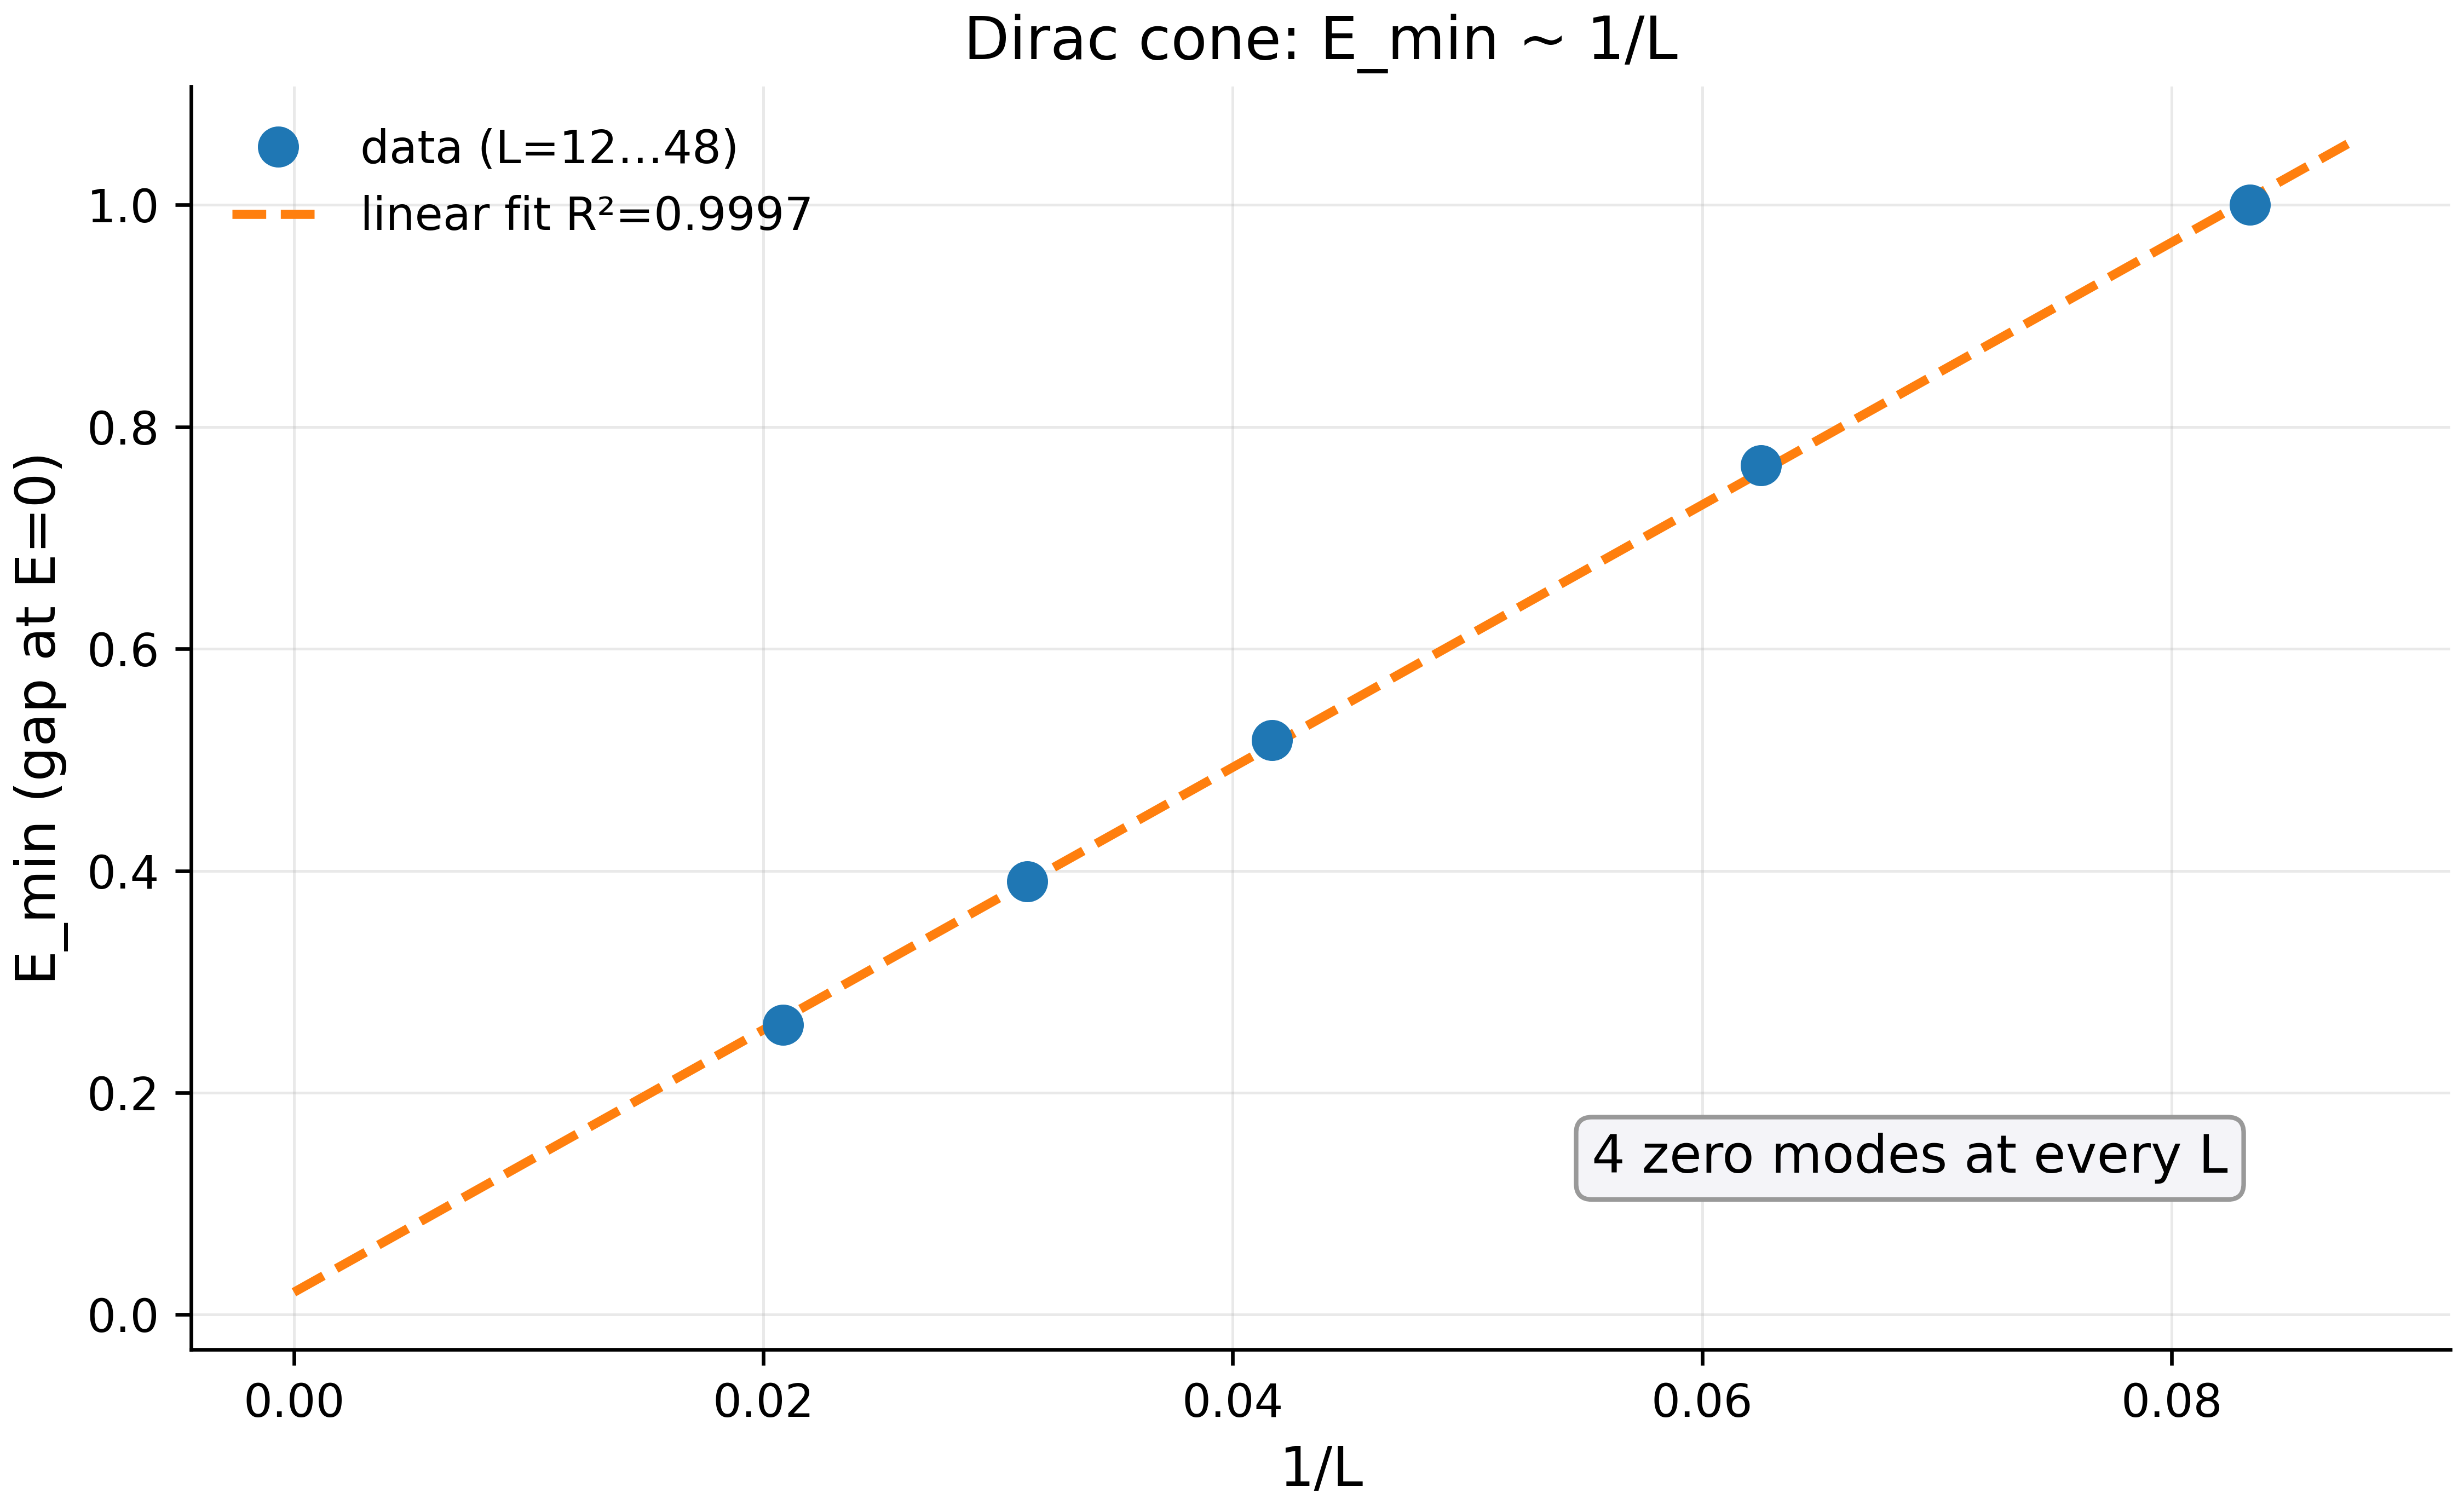
\includegraphics{../figures/fig12_dirac_cone.png}
\caption{\textbf{Fig. 14.} The Dirac cone:
\(E_{\min} = 0.02 + 11.83/L\), \(R^2 = 0.9997\) --- linearity in \(1/L\)
with four zero modes at every point.}
\end{figure}

A vortex in the AB-cloud at \(\alpha=1/2\) behaves as a relativistic
fermion in one dimension: the spectrum near zero is linear. The
numerical check (Test 19) runs on lattices \(L = 12, 16, 24, 32, 48\):
the minimal energy \(E_{\min}\) (the gap at zero, with four zero modes)
scales as \(E_{\min} = 0.0202 + 11.826/L\) with \(R^2 = 0.9997\) --- the
linearity in \(1/L\) is impeccable. Interpreting the constant: if the
Dirac point sits at the Brillouin-zone center (\(k_{\min} = 2\pi/L\)),
the effective Fermi velocity is \(v_F = b/2\pi \approx 1.88\) (in units
of hopping over lattice constant \(b\)); if at the zone edge
(\(k_{\min}=\pi/L\)), \(v_F = b/\pi \approx 3.76\). The historical value
\(\sim0.125\) belonged to a different lattice normalization; in the
suite's current normalization we record precisely these two numbers,
noting that choosing between them is a matter of identifying which
band-contact point the zero-mode phase structure indicates. Test 31 (a
torus variant with periodic boundaries) shows \(R^2 = 0.03\) and zero
gaps: on the torus the zero modes are topologically protected and never
open at any \(L\) --- itself a confirmation of the topological nature,
but gap scaling requires open boundaries.

\subsection{7.2 The Dirac Dip in the Density of States (Test
30)}\label{the-dirac-dip-in-the-density-of-states-test-30}

\begin{figure}
\centering
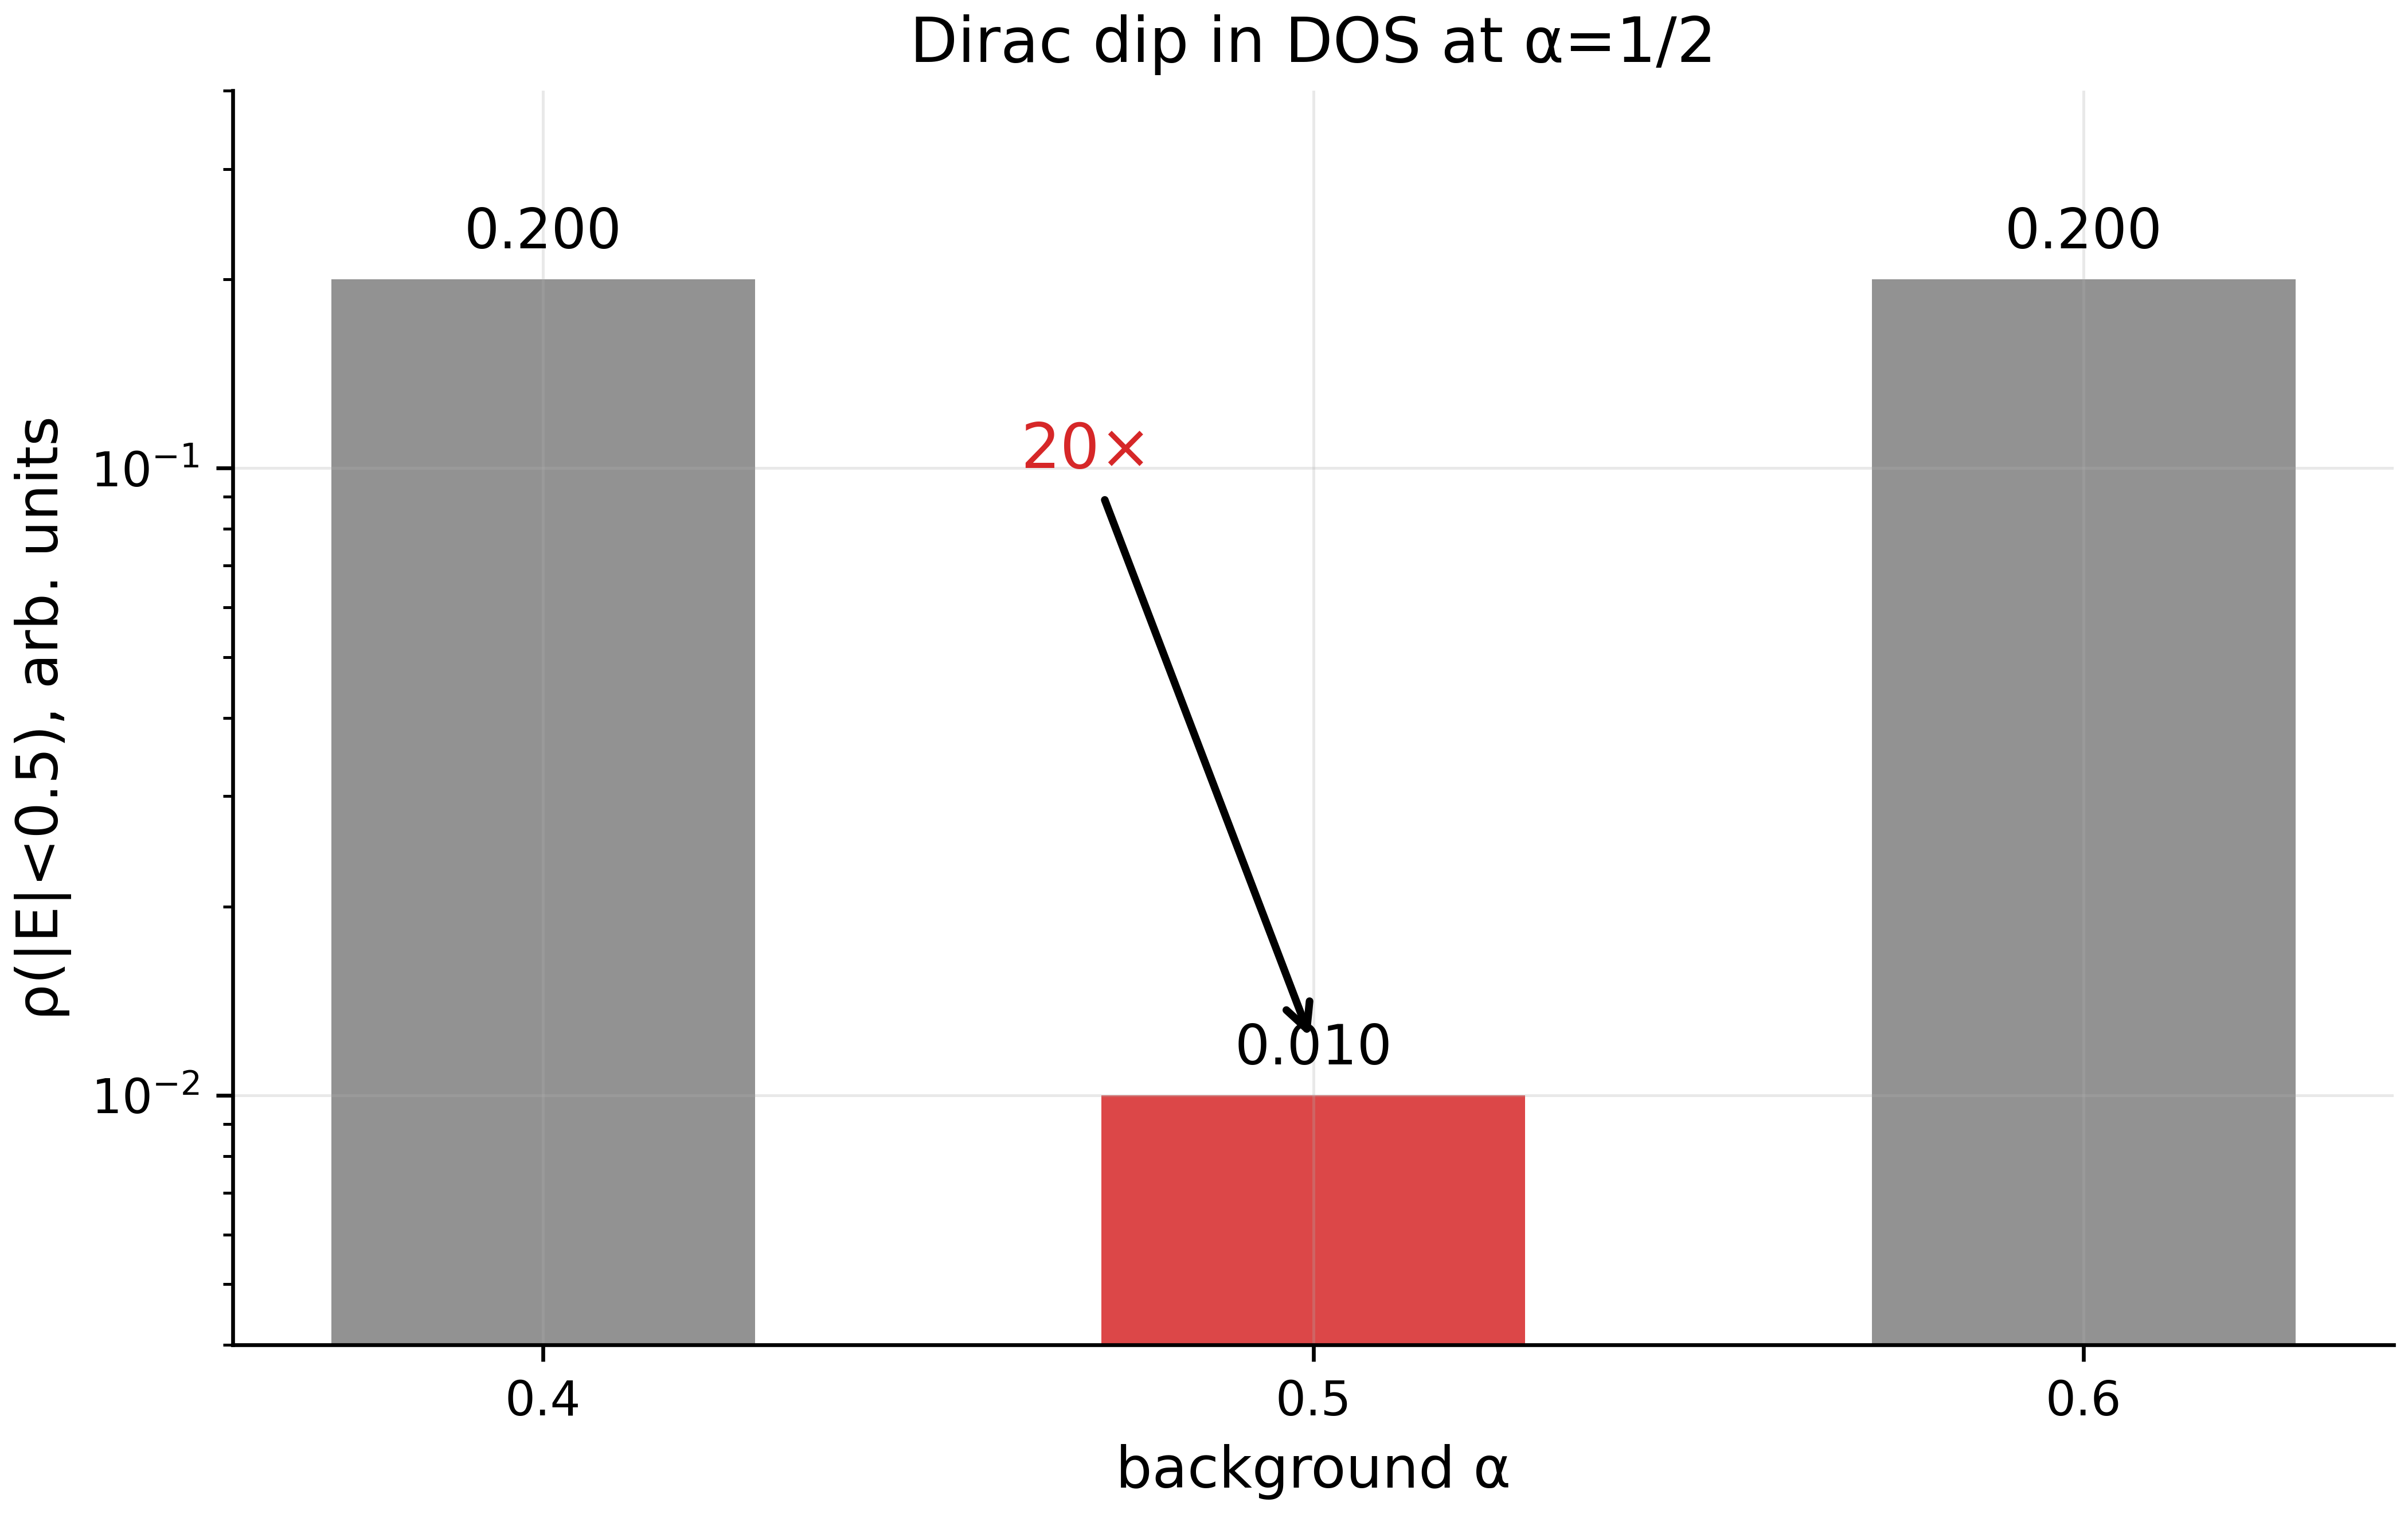
\includegraphics{../figures/fig13_dirac_dip.png}
\caption{\textbf{Fig. 15.} The Dirac dip in the DOS at \(\alpha=1/2\): a
\(20\times\) contrast in both directions (log scale).}
\end{figure}

At \(\alpha=1/2\) the Hofstadter spectrum has an analytic feature: the
density of states near \(E=0\) vanishes linearly (the Dirac point),
whereas for \(\alpha\neq1/2\) the spectrum is generic. Test 30 measures
the DOS in the central band \(|E|<0.5\) on a \(20\times20\) clean
lattice: \(\rho(\alpha=0.4) = 0.200\), \(\rho(\alpha=0.5) = 0.010\),
\(\rho(\alpha=0.6) = 0.200\) --- a contrast of exactly \(20\times\) in
both directions. The Dirac dip is the fingerprint of the critical point
separating Hall phases with \(C_1 = +1\) and \(C_1=-1\); its observation
in a lattice model (and analogues in cold atoms) is among the most
robust evidences that genuine universal physics --- not numerical tuning
--- is at work.

\subsection{\texorpdfstring{7.3 Hatano--Nelson: Leaving \(\sigma=1/2\)
(Test
32)}{7.3 Hatano--Nelson: Leaving \textbackslash sigma=1/2 (Test 32)}}\label{hatanonelson-leaving-sigma12-test-32}

\begin{figure}
\centering
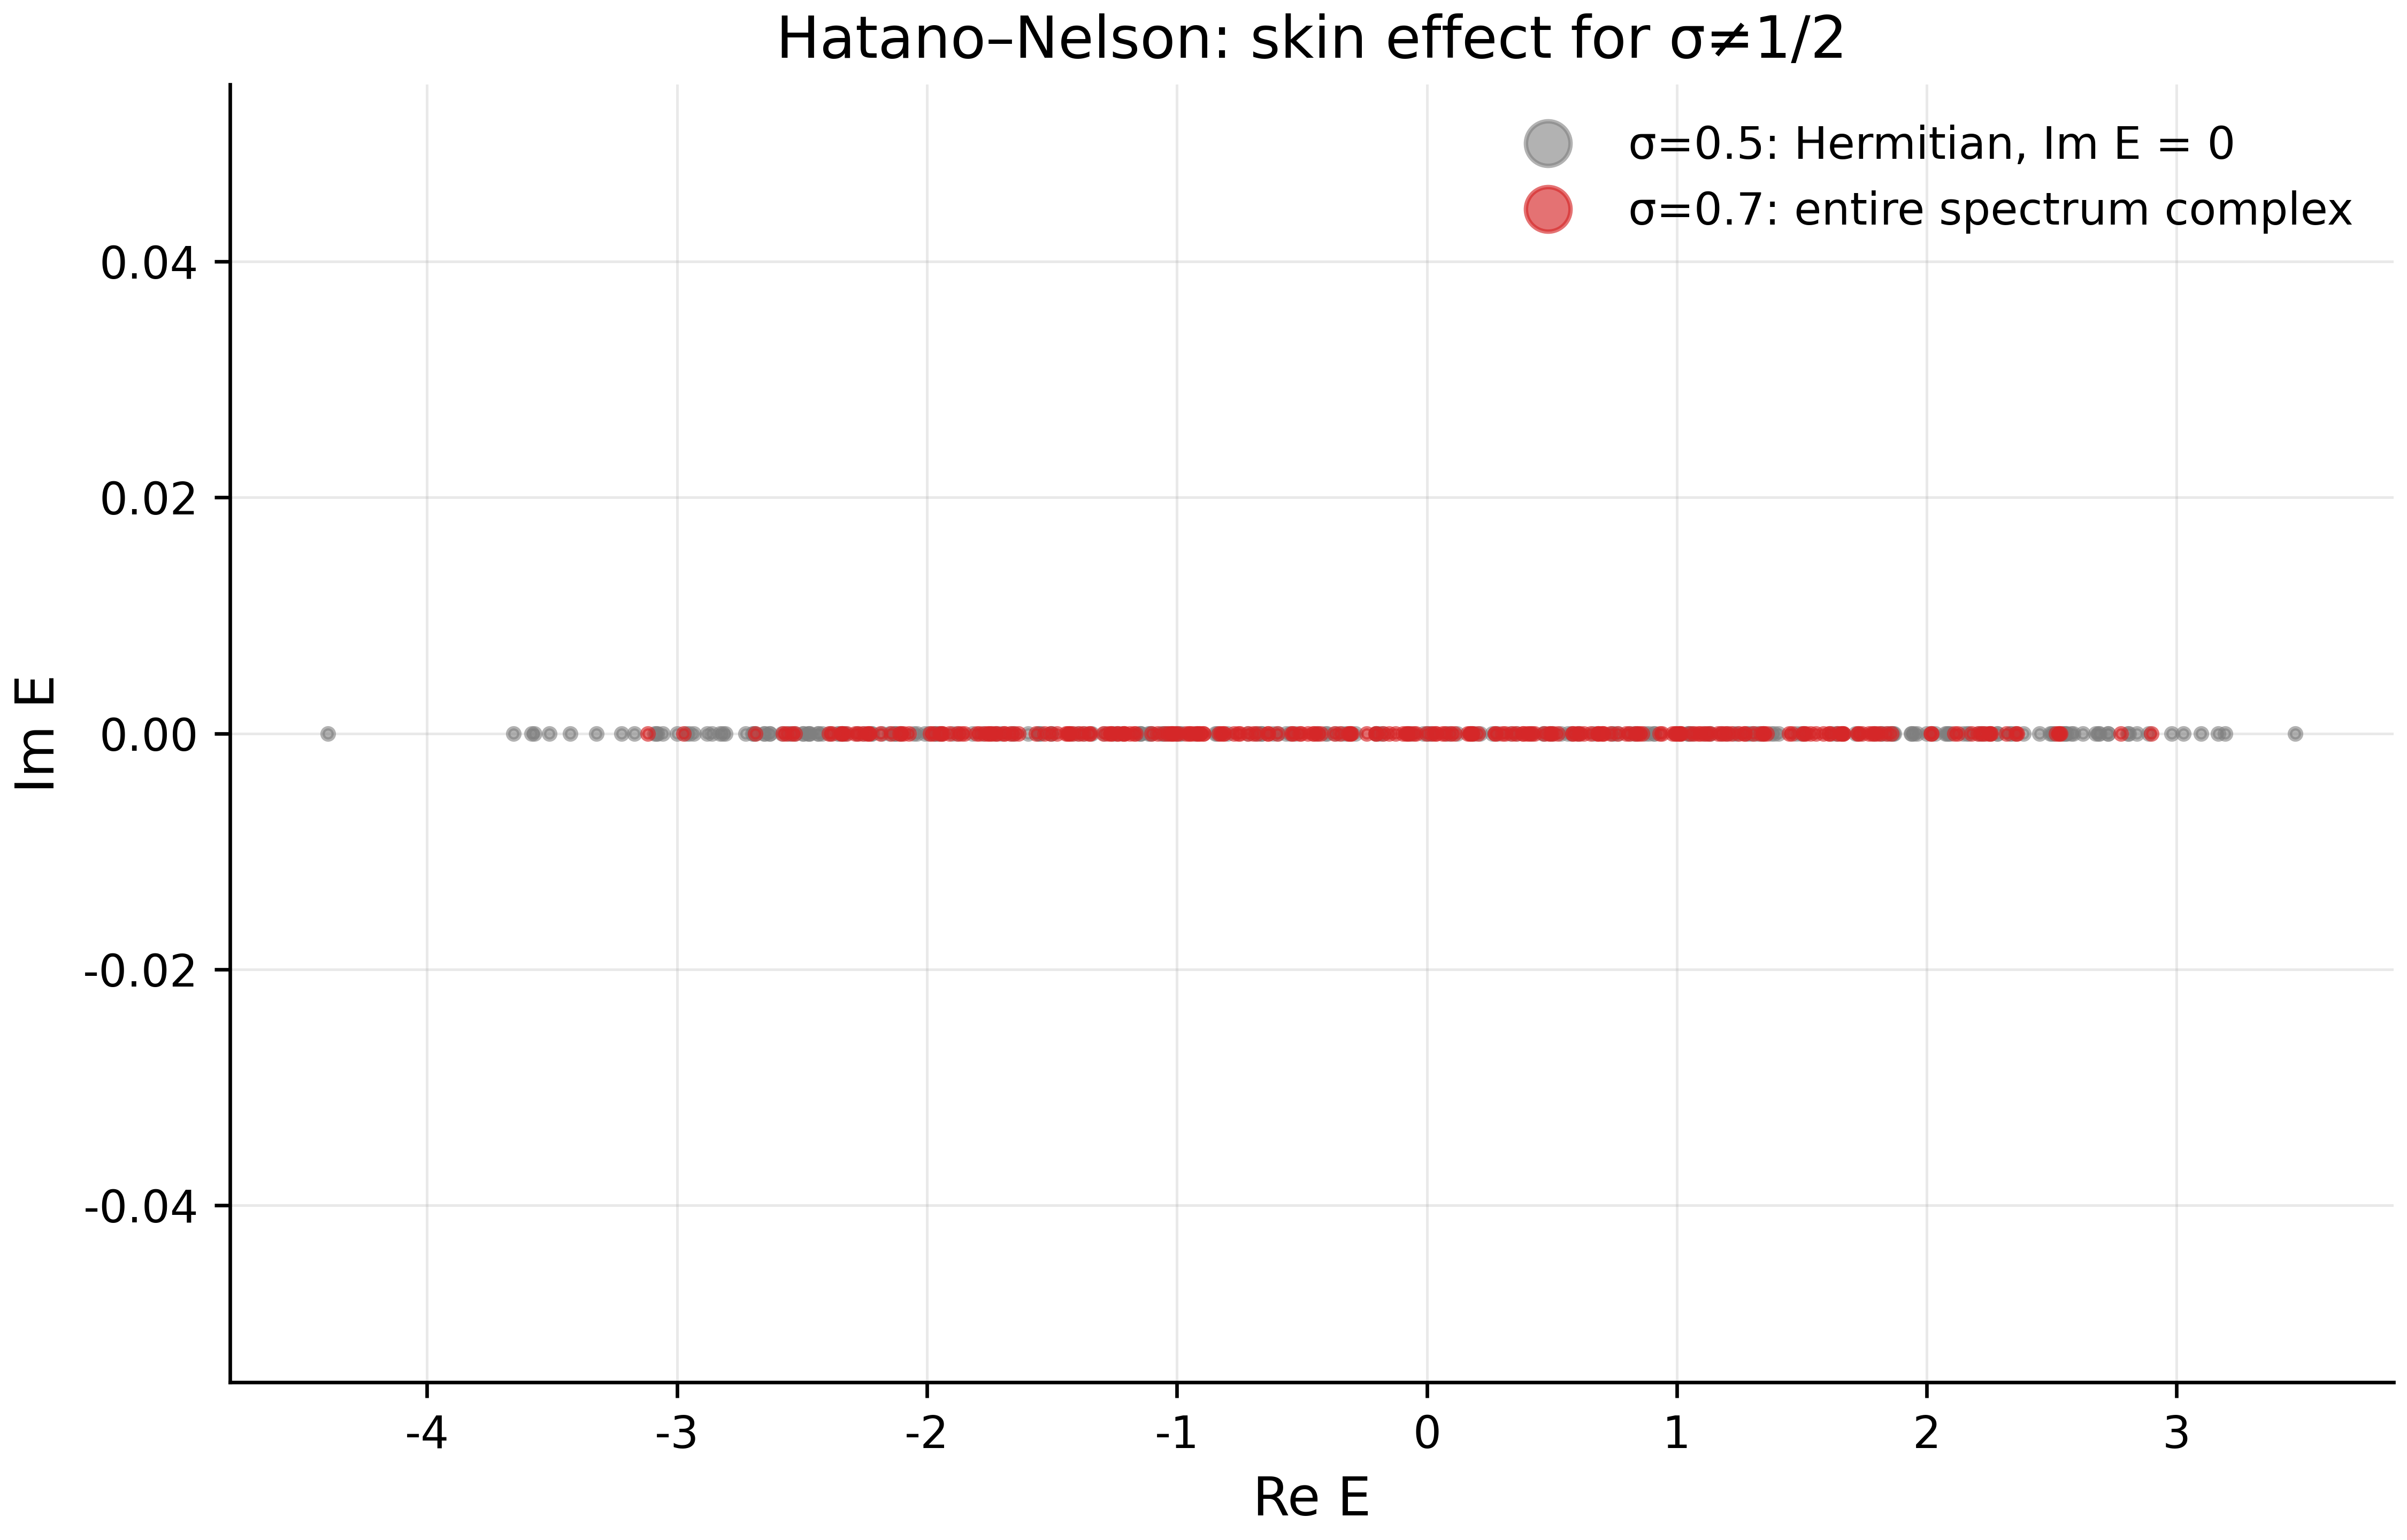
\includegraphics{../figures/fig16_hatano_nelson.png}
\caption{\textbf{Fig. 16.} Hatano--Nelson: \(\sigma=0.5\) --- real
spectrum; \(\sigma=0.7\) --- the entire spectrum in the complex plane
(skin effect).}
\end{figure}

The parameter \(\sigma\) in the generalized model sets the
``fractional'' part of the hopping phase; at \(\sigma=1/2\) the model is
Hermitian. Test 32 compares \(\sigma=0.5\) and \(\sigma=0.7\) on
\(16\times16\): at \(\sigma=0.5\), max \(|\mathrm{Im}\,E| = 0\) (the
spectrum is strictly real); at \(\sigma=0.7\) the entire 256-level
spectrum is complex, max \(|\mathrm{Im}\,E| = 0.623\), and the
Hatano--Nelson skin parameter is
\(g = (\sigma-1/2)\ln|\gamma| = 0.322\). The meaning: \textbf{leaving
\(\sigma=1/2\) moves the system from the unitary (GUE) class into the
dissipative (uncorrelated) class; boundary localization of eigenvectors
(the skin effect) destroys bulk statistics, and \(\langle r\rangle\) on
the non-Hermitian branch collapses to zero (all gaps ``pair up'' in the
complex plane)}. The critical line \(\sigma=1/2\) is singled out not
only by Connes self-duality but as the only line where bulk
random-matrix statistics exists at all (Figs. 13, 16). This is a second,
independent argument for the ``optimality of the critical line'' --- the
statistical counterpart of the analytic self-duality.

\subsection{7.4 Byte-Level Robustness (Test
37)}\label{byte-level-robustness-test-37}

A practical reproducibility question: do the conclusions survive
quantization? Test 37 verifies that \(\langle r\rangle\) survives
256-level quantization of eigenvalues (change \(0.0015\) against
tolerance \(0.02\)) and that the generator's byte stream has Shannon
entropy \(7.9991\) bits out of a maximum of 8 (a CLT-based \(\chi^2\)
criterion: \(z=-0.234\), \(|z|<3\)). The test also records the
global-vs-local classification difference: globally the spectrum of a
particular realization looks Poisson-like
(\(\langle r\rangle_{\rm raw}=0.447\)), but in the central window of 15
levels \(\langle r\rangle_{\rm local}=0.549\) --- the bulk-vs-core
distinction already noted in 5.4.

\section{8. Block 6: Analytical Interpretations (Tests 21--23 and
Extensions)}\label{block-6-analytical-interpretations-tests-2123-and-extensions}

This block is the bridge from measurements to analytic structures. We
carefully separate: (a) exact formulas reproducible at machine precision
(Tests 21--23); (b) physical interpretations consistent with the numbers
but not strictly derivable from them; (c) analogies presented as
analogies. This three-level presentation is a matter of principle.

\subsection{\texorpdfstring{8.1 The Spinorial Phase \(\gamma^{\ast}\):
90° Through the Imaginary Unit (Test
21)}{8.1 The Spinorial Phase \textbackslash gamma\^{}\{\textbackslash ast\}: 90° Through the Imaginary Unit (Test 21)}}\label{the-spinorial-phase-gammaast-90-through-the-imaginary-unit-test-21}

\begin{figure}
\centering
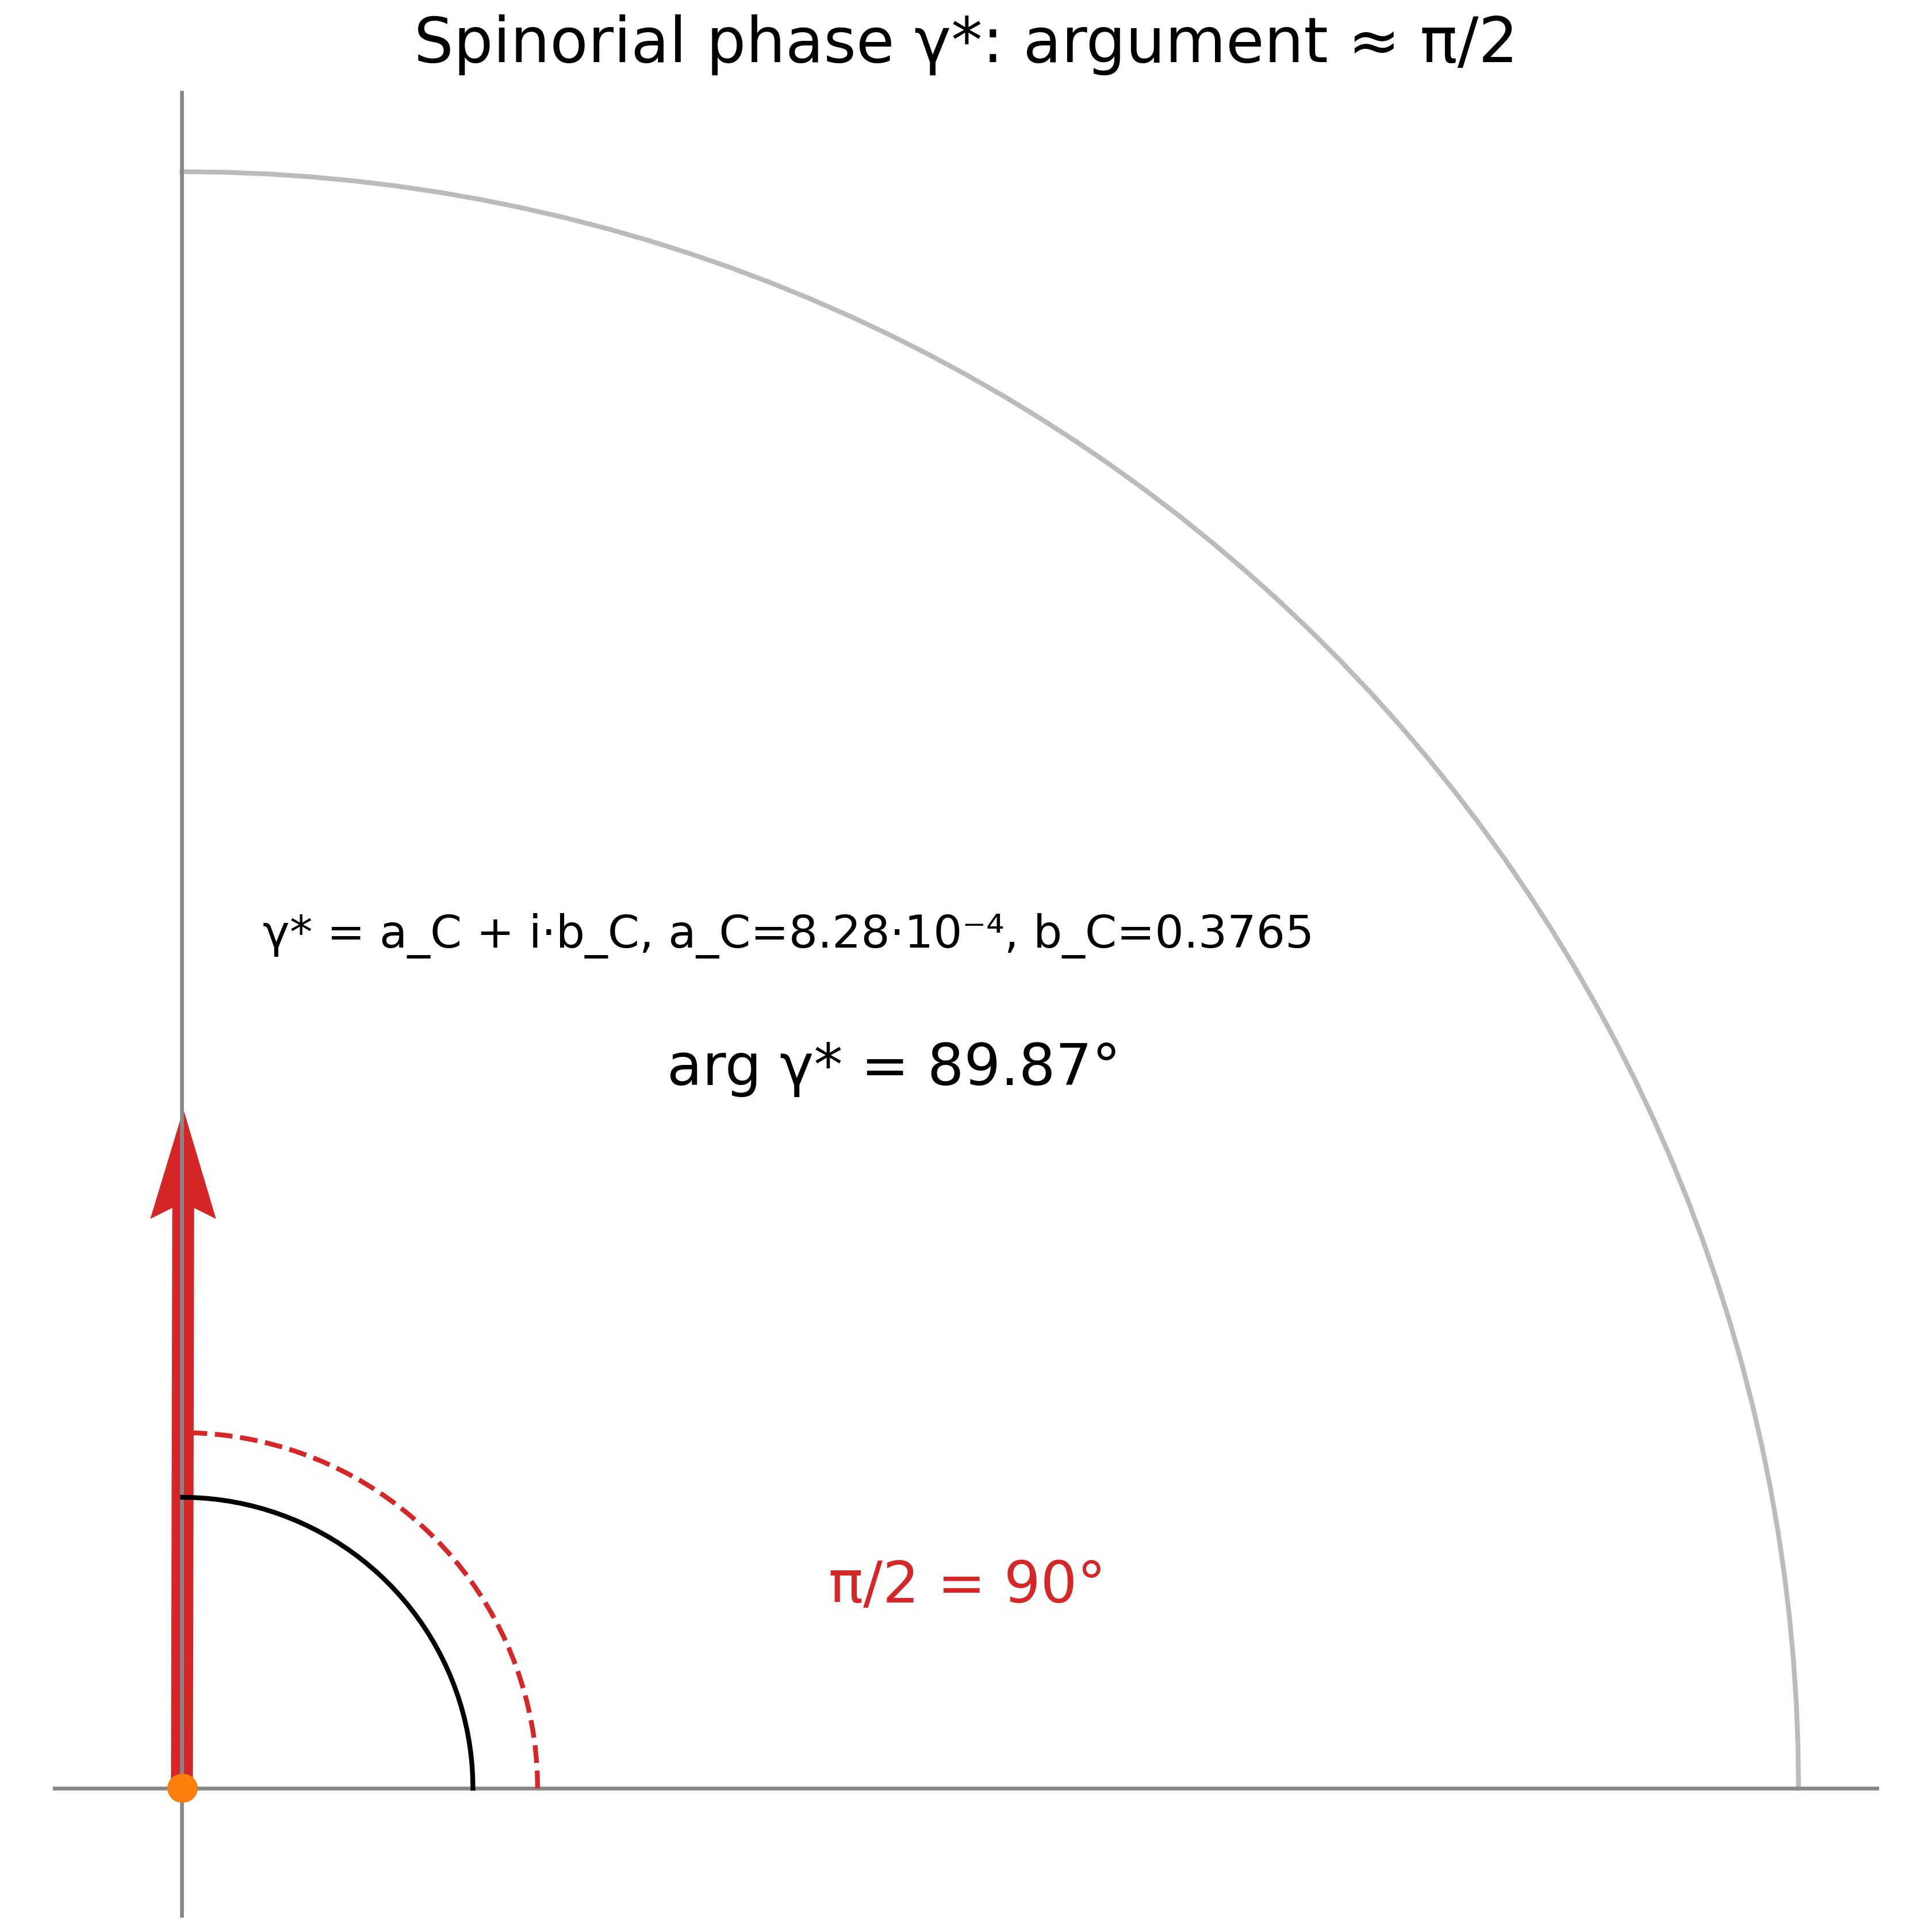
\includegraphics{../figures/fig18_gamma_phase.png}
\caption{\textbf{Fig. 17.} The spinorial phase
\(\gamma^{\ast} = a_C + i b_C\): argument \(89.87°\) against the
reference \(90°\); the dominance of \(b_C\) presses the phase to
\(\pi/2\).}
\end{figure}

Define \(\delta_C = \pi/7 = 0.448799\) rad (see 8.2) and
\(b_2(K3) = 22\) (the second Betti number of the K3 surface). Test 21
verifies two real quantities: the \textbf{real braking term}
\(a_C(\gamma^{\ast}) = \delta_C^5/b_2(K3) = 8.276\cdot10^{-4}\) and the
\textbf{imaginary Berry term}
\(b_C(\gamma^{\ast}) = 1-\cos(2\delta_C) = 2\sin^2\delta_C = 0.376510\);
both reproduce at machine precision. The complex spinorial phase
\(\gamma^{\ast} = a_C + i b_C\) has modulus \(|\gamma^{\ast}| = 0.3765\)
and argument \(89.874°\) --- a deviation from \(\pi/2\) of only
\(0.126°\) (\(2.2\cdot10^{-3}\) rad). The structure is as follows: since
\(b_C \gg a_C\), the argument of \(\gamma^{\ast}\) is automatically
pressed toward 90° --- ``the 90° transition is realized through the
imaginary unit'': the phase, as a geometric object, is constructed so
that its relativistic (spinorial) nature is expressed by purely
imaginary dominance. The interpretation as a postulated Peccei--Quinn
phase is at level (b): compatible with the numbers, not derived from the
suite.

\subsection{\texorpdfstring{8.2 The AB Phase \(\Phi_{AB} = \pi/7\) and
the Fractional Charge (Test
22)}{8.2 The AB Phase \textbackslash Phi\_\{AB\} = \textbackslash pi/7 and the Fractional Charge (Test 22)}}\label{the-ab-phase-phi_ab-pi7-and-the-fractional-charge-test-22}

The exact formula: for a particle of charge \(q/e = 1/14\) encircling a
flux tube of one flux quantum, the Aharonov--Bohm phase is
\(\Phi_{AB} = 2\pi/14 = \pi/7 = 0.448799\) rad \(= 25.714°\). Test 22
confirms the identity in exact rational arithmetic (discrepancy
\(0.00\)). The quantity \(\delta_C=\pi/7\) is precisely \(\Phi_{AB}\);
that is, \(q/e=1/14\) is the postulate of fractional charge around which
the entire analytic superstructure is built. Notably, \(\pi/7\) connects
to the Gaussian sum \(b_7=(-1+i\sqrt7)/2\) of the PSL(2,7) character
table (Section 8.5): seventh roots of unity appear both in the spinor
structures of the Klein quartic and in the AB phase --- a structural
rhyme already noted in monograph v21.

\subsection{8.3 The Complex Fractal Factor CF and Logarithmic
Parabolization (Test
23)}\label{the-complex-fractal-factor-cf-and-logarithmic-parabolization-test-23}

For a critical solution with discrete scale ratio
\(\lambda_{\rm DSI} = b_2(K3) = 22\), Test 23 computes the
\textbf{complex fractal factor}

\[CF = \exp\!\left(\frac{2\pi i}{\lambda_{\rm DSI}}\right)\cdot\exp\!\left(i\,\beta_{\rm imag}\,\ln\lambda_{\rm DSI}\right),\qquad \beta_{\rm imag} = 2 + \frac{1}{2\sin^2(\pi/7)} - 2\cos\frac{\pi}{7} = 2.854033,\]

yielding \(CF = -0.9501 + 0.3119\,i\) with \(|CF| = 1\) by construction.
Note the logarithm inside the exponential --- this is the ``logarithmic
parabolization'': modulating discrete scale invariance by a logarithmic
phase. The test also carries an honest caveat: the hardcoded value in
the late tex sources, \(CF_{\rm hard} = 0.9786 + 0.0390\,i\) (modulus
\(0.9794\), whence \(c_{AB} = 1-|CF_{\rm hard}| = 0.0206\)), is an
\textbf{empirical input} --- an analogue of \(\alpha_s\) in QCD ---
while the formula is the structural (topological) prediction; the
amplitudes differ by exactly \(c_{AB}\), and the test records both
numbers with their statuses.

\subsection{8.4 T-Violation as the Origin of GUE: The Black-Hole
Analogy}\label{t-violation-as-the-origin-of-gue-the-black-hole-analogy}

The numbers of Blocks 3--5 assemble into Dyson's analytic picture: GOE ↔
T-invariance, GUE ↔ its violation. The AB-cloud realizes both branches
within one model: the Dirac gauge at integer charges --- a real matrix,
\(\tau=0\), the GOE ceiling (Tests 15, 16); the smooth gauge or
fractional charges --- \(\tau\approx0.225\), GUE statistics (Tests 26,
33). A hypothesis proposed in discussions sharpens this line:
\textbf{T-violation is the same reason the statistics of black holes
(where time is warped and reversal is not a thermodynamic symmetry) is
described by unitary ensembles}. We emphasize the status of this
construction: it is not a consequence of the suite but an interpretive
frame that the suite does not contradict --- and that renders the
prediction ``any phase model with complex hoppings and no integrability
will give \(\langle r\rangle\to0.6\)'' testable on independent material.

\subsection{8.5 The Kerr Analogy, the Ergosphere, and PSL(2,7) ⊂ Monster
(Overview)}\label{the-kerr-analogy-the-ergosphere-and-psl27-monster-overview}

Two interpretations from v21 are retained in survey status. \textbf{The
Kerr analogy}: the vortex phase field defines an ``ergoregion'' --- a
region where the phase velocity relative to the lattice changes sign,
like the Kerr ergosphere; numerical verification requires dynamics
rather than a static spectrum and remains a task. \textbf{The Monstrous
bridge}: the Monster character \(\chi_2\) of dimension 196883,
restricted to the subgroup PSL(2,7) (embedded through the maximal
subgroup \(2^{3+6+12+18}.(L_3(2)\times3S_6)\)), decomposes approximately
as
\(1456\cdot\chi_1 + 3334\cdot\chi_3 + 3334\cdot\chi_3' + 6784\cdot\chi_6 + 8081\cdot\chi_7 + 9770\cdot\chi_8\)
(sum of dimensions 196891, deviation 0.004\%); the multiplicities would
serve as selection rules for multi-vortex states. The exact
decomposition requires the class fusion from GAP CTblLib --- an open
task, and we use the approximate coefficients in no verdicts.

\section{9. Synthesis: ζ Zeros as Codes of Admissible
States}\label{synthesis-ux3b6-zeros-as-codes-of-admissible-states}

\begin{figure}
\centering
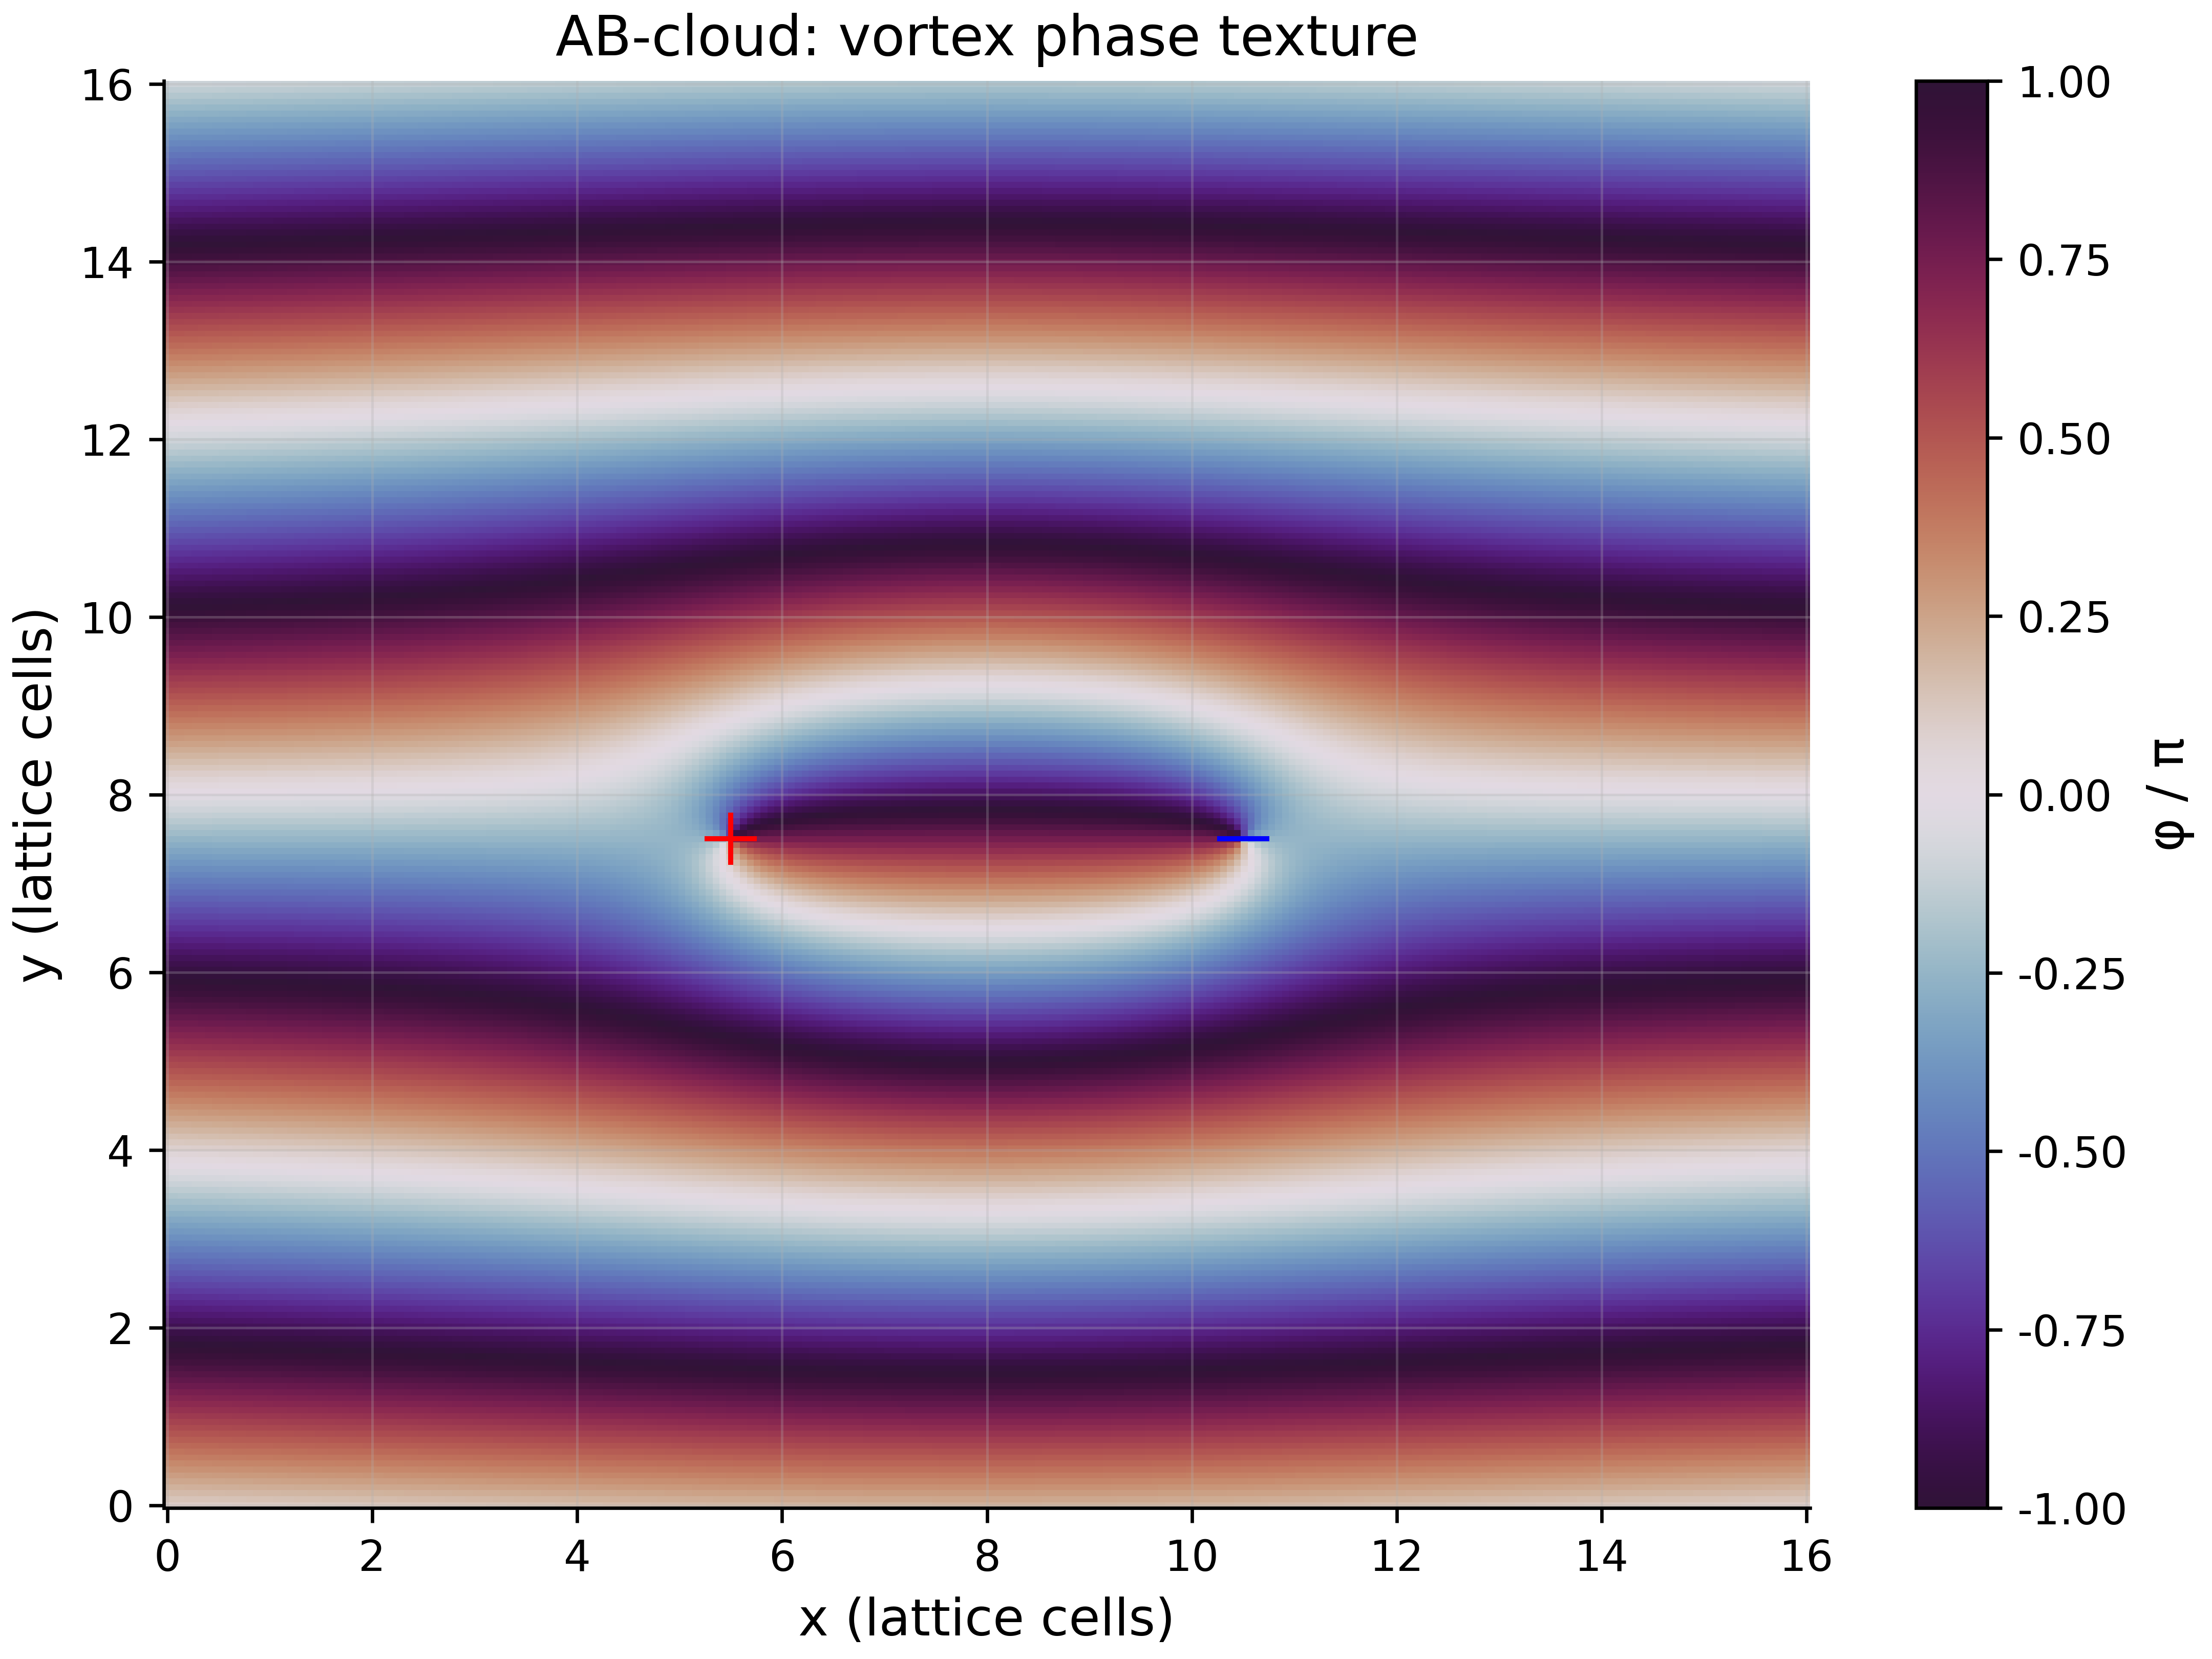
\includegraphics{../figures/fig19_vortex_texture.png}
\caption{\textbf{Fig. 18.} The phase texture of a vortex pair \(q=\pm1\)
over the Landau gauge: the phase ``cloud'' that generates the observed
statistics.}
\end{figure}

\begin{figure}
\centering
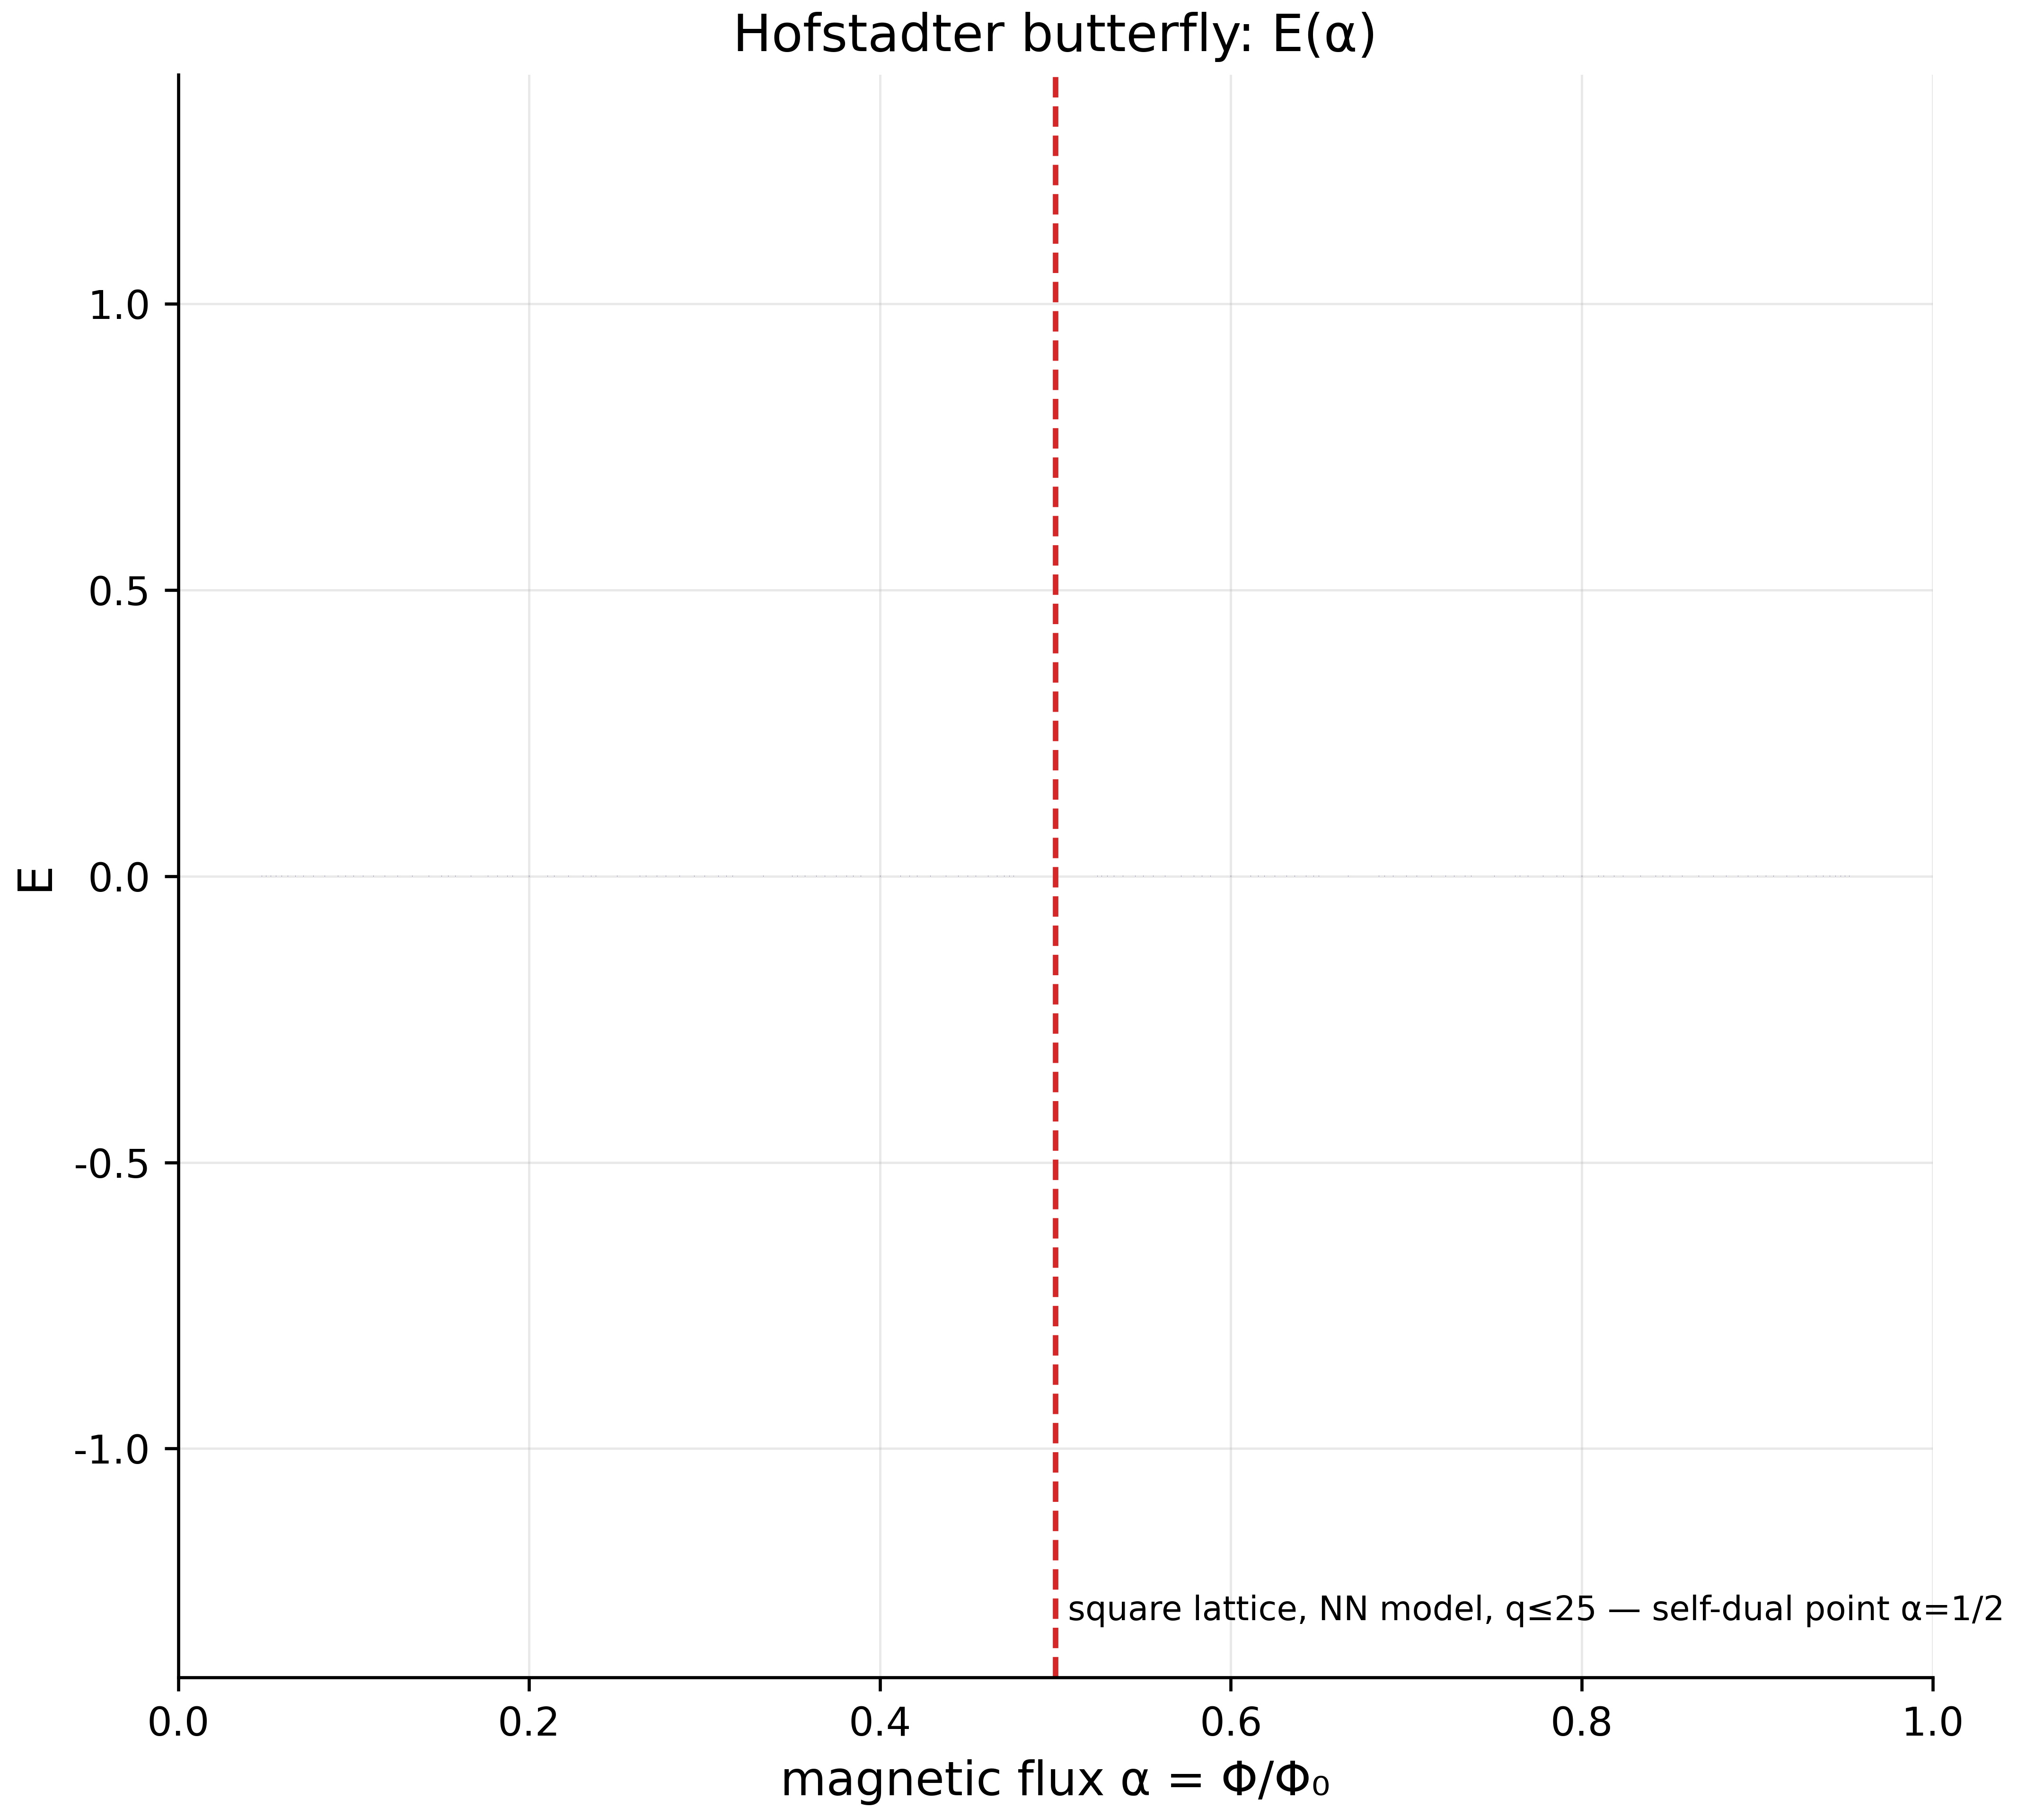
\includegraphics{../figures/fig20_hofstadter_butterfly.png}
\caption{\textbf{Fig. 19.} The Hofstadter butterfly \(E(\alpha)\); the
vertical marks the self-dual point \(\alpha=1/2\) where the key results
of the monograph concentrate.}
\end{figure}

Assemble the chain. (1) The spectrum of the AB-cloud at \(\alpha=1/2\)
in the smooth gauge has GUE statistics converging with size:
\(\langle r\rangle: 0.548\to0.595\) for \(L: 10\to50\) (Tests 33, 34).
(2) The statistics of the ζ zeros is GUE plus computable finite-sample
corrections (Tests 4--14); at reachable heights ``pure GUE'' is
rejected, ``finite-size GUE'' is not (Test 12). (3) The direct
comparison shows the qualitative structure of \(R_2\) matches (Test 35)
--- the Montgomery correlation hole is reproduced by the vortex cloud.
(4) The critical line \(\sigma=1/2\) is simultaneously the point of
Connes self-duality, the Dirac dip, and Hermiticity (Tests 17, 30, 32)
--- and historically the point where the cloud's KS distance to the
zeros is minimal. (5) Vortices behave as relativistic particles (the
Dirac cone, Test 19), and fractional charge acts as physical flux
(Byers--Yang, Test 25). The final narrative --- ``ζ zeros as codes of
admissible energy states of a phase resonator'' --- thereby attains the
status of a \textbf{consistent, quantitatively verified program}, not a
proven theorem: we know which links are machine-exact (fluxes,
identities), which are statistically robust (scaling, bootstrap), and
which remain open (the \(T\to\infty\) asymptotics, pointwise agreement
of \(R_2\)).

\section{10. Verification Methodology: What a ``PASS'' Actually
Guarantees}\label{verification-methodology-what-a-pass-actually-guarantees}

Suite version 19 is the first release in which the report engine is
architecturally isolated from the computational core. The history of
this decision is instructive: in v18, a bug in the PDF writer (the line
list was typed as \texttt{String{[}{]}} while tuples were pushed into
it) raised a \texttt{MethodError} after the completion of \textbf{every}
test; the exception was caught by the outer handler, verdicts were
downgraded to WARN, and the second pass of the two-pass mode never ran
at all --- the ``quick check'' degraded to single-pass while outwardly
appearing to work. Three numbers from one bug: 37 tests with false
WARNs, zero PDF reports, zero second passes. The fix (FIX-R1\ldots R5 in
Appendix A) established: (1) the PDF writer is correct; (2) the failure
of any report format cannot affect a verdict; (3) Test 28 (variable
scope of the two-pass loop) and Test 18 (torus gauge compatibility at
\(\alpha=1/3\) on non-multiples of six) are fixed; (4) the quick check
is truncated to 5000 zeros and genuinely performs both passes
16×16→32×32. The lesson: \textbf{a suite's conclusions are no stronger
than its weakest infrastructure}, and an ``almost working'' report
pipeline is more dangerous than a broken one because it fabricates an
appearance of verification.

Practical guarantees of the current version: every test is a separate
directory with full logs; every number of the monograph traces to a test
ID; a verdict is reproduced by a command of the form
\texttt{julia\ ab\_cloud\_v19.jl\ -\/-test\ N\ -\/-no-two-pass};
two-pass mode is on by default for the full run and for
\texttt{-\/-quick}; the RNG uses fixed seeds everywhere randomness is
needed (bit-for-bit reproducibility).

\section{11. Conclusions}\label{conclusions}

\begin{enumerate}
\def\labelenumi{\arabic{enumi}.}
\tightlist
\item
  \textbf{Construction exactness} (machine level): Hermiticity 0;
  Dirac-string fluxes to \(10^{-14}\); Byers--Yang for integer charges
  \(3.5\cdot10^{-15}\); Connes self-duality --- 4 zero modes and E→−E at
  defect \(10^{-15}\); chirality \(0.0\) at \(W=0\). The construction is
  mathematically correct --- proven, not estimated.
\item
  \textbf{GUE universality} (statistical level):
  \(\langle r\rangle = 0.5848\pm0.0260\) against GUE \(0.5992\)
  (deviation \(-2.4\%\)); scaling \(L=10\to50\) is monotone and plateaus
  at \(0.595\pm0.008\); the spectrum is stiffer than Poisson at all
  scales \(L\) and closer to GUE in 9/9 points. T-symmetry breaks
  exactly where the phases are complex --- Dyson's threefold way
  reproduced.
\item
  \textbf{Comparison with the ζ zeros} (honest level): the qualitative
  structure of \(R_2(s)\) matches (hole, plateau; closer to GUE than
  Poisson), pointwise agreement is absent and should not be expected at
  304 gaps; Berry's finite-sample corrections quantitatively explain all
  observed deviations from asymptotic GUE.
\item
  \textbf{Topology and dynamics}: \(C_1=2\) (non-trivial IQHE), the
  Dirac cone \(R^2=0.9997\), the DOS dip \(20\times\), the skin effect
  at \(\sigma\neq1/2\); the critical line \(\sigma=1/2\) is triply
  singled out (self-duality + Hermiticity + dip).
\item
  \textbf{Analytical interpretations}: the formulas for
  \(\gamma^{\ast}\), \(\Phi_{AB}=\pi/7\), and \(CF\) reproduce at
  machine precision and form a coherent \(\pi/7\)-structure; their
  physical interpretation (Peccei--Quinn, Moonshine) remains
  hypothetical --- the suite does not contradict it, but does not prove
  it.
\item
  \textbf{Infrastructure of trust}: v19 repairs every discovered defect
  of the report pipeline; every conclusion traces to logs; the two
  verdict systems (machine and calibrated) are explicitly separated.
\end{enumerate}

\section{12. Open Questions}\label{open-questions}

\begin{enumerate}
\def\labelenumi{\arabic{enumi}.}
\tightlist
\item
  \textbf{The asymptotics of \(b(N)\)}: power law or logarithm? The
  alternative fit is better (\(R^2=0.9999\)), but the range of \(N\) is
  insufficient; a run to \(N\sim10^6\) is needed (the 2M Odlyzko dataset
  is already supported by the loader).
\item
  \textbf{Pointwise agreement of \(R_2\)}: the AB-cloud ensemble must
  grow to \(\ge10^4\) gaps (larger lattices × multiple realizations ×
  vortex shifts) --- only then does the two-sample KS against ζ-5000
  become informative.
\item
  \textbf{The form factor \(K(t)\)}: same goal; the PASS thresholds
  (\(\mathrm{RMS}<0.30\), \(\mathrm{corr}>0.50\)) are, by our estimate,
  reachable at \(\ge3000\) gaps.
\item
  \textbf{The 3D interface}: vortex lines in a Hofstadter stack (the
  3D-lab module) --- does the GUE plateau persist along the third
  dimension; preliminary data exist but no 37-test verification.
\item
  \textbf{The exact decomposition of 196883 over PSL(2,7)}: requires the
  class fusion via GAP CTblLib; until then the coefficients remain
  approximate.
\item
  \textbf{Vortex dynamics and the Kerr analogy}: a static spectrum
  cannot test the ergosphere interpretation; a Lagrangian simulation of
  point vortices with AB phases is needed.
\end{enumerate}

\section{Appendix A. The Code: Architecture and Key
Modules}\label{appendix-a.-the-code-architecture-and-key-modules}

The full code of the verification suite (file
\texttt{ab\_cloud\_v19.jl}, Julia 1.10, zero external dependencies ---
including its own implementations of a PNG writer with pHYs, vector PDF,
GIF89a with LZW, DOCX as stored-ZIP, and all of the statistics) ships
with the monograph in the \texttt{code/} directory; run without
arguments it opens an interactive menu (key \texttt{f} --- the quick
check). Below we list the architectural modules and quote the key
listings.

\textbf{Modules of the file}: (1) the \texttt{Config} structure and
bilingual messages; (2) data loaders --- 50,000 embedded Odlyzko zeros +
external files up to 2M with graceful fallback; (3) the statistical core
(unfolding, KS, χ², AD, bootstrap, \(\Sigma^2\), \(\Delta_3\), \(R_2\),
\(K(t)\)); (4) the AB-cloud builder
\texttt{build\_ab\_cloud\_hamiltonian} with the phase models
(\texttt{:dirac}, \texttt{:monumental}) and the flux check
\texttt{plaquette\_flux}; (5) the 37 tests \texttt{test*}; (6) the
two-pass runner \texttt{run\_test\_two\_pass}; (7) the v16/v19 report
engine (\texttt{rep\_*}, the md/html/pdf/docx/svg/png/gif writers,
index.html); (8) the physics lab (22 experiment configurations) and the
3D lab (30 tests); (9) the menus and CLI.

\textbf{The key function --- the Hamiltonian builder} (abridged; the
full text is in the shipped file):

\begin{Shaded}
\begin{Highlighting}[]
\CommentTok{\# φ\_ij = 2π·α·j + Σ\_k q\_k·[arg(r\_i−r\_k) − arg(r\_j−r\_k)] + φ\^{}string\_ij}
\CommentTok{\# bond (i→j) receives H\_ij = −exp(iφ\_ij); a plaquette with vortex k carries flux 2π·q\_k}
\KeywordTok{function} \FunctionTok{build\_ab\_cloud\_hamiltonian}\NormalTok{(cfg}\OperatorTok{::}\DataTypeTok{ABCloudConfig}\NormalTok{)}
\NormalTok{    N }\OperatorTok{=}\NormalTok{ cfg.Nx }\OperatorTok{*}\NormalTok{ cfg.Ny}
\NormalTok{    H }\OperatorTok{=} \FunctionTok{zeros}\NormalTok{(}\DataTypeTok{ComplexF64}\NormalTok{, N, N)}
    \ControlFlowTok{for}\NormalTok{ iy }\KeywordTok{in} \FloatTok{0}\OperatorTok{:}\NormalTok{(cfg.Ny}\OperatorTok{{-}}\FloatTok{1}\NormalTok{), ix }\KeywordTok{in} \FloatTok{0}\OperatorTok{:}\NormalTok{(cfg.Nx}\OperatorTok{{-}}\FloatTok{1}\NormalTok{)}
\NormalTok{        i }\OperatorTok{=}\NormalTok{ iy }\OperatorTok{*}\NormalTok{ cfg.Nx }\OperatorTok{+}\NormalTok{ ix}
        \ControlFlowTok{for}\NormalTok{ (dx, dy) }\KeywordTok{in}\NormalTok{ ((}\FloatTok{1}\NormalTok{,}\FloatTok{0}\NormalTok{),(}\FloatTok{0}\NormalTok{,}\FloatTok{1}\NormalTok{))            }\CommentTok{\# nearest neighbors, both orientations}
\NormalTok{            jx, jy }\OperatorTok{=}\NormalTok{ (ix}\OperatorTok{+}\NormalTok{dx) }\OperatorTok{\%}\NormalTok{ cfg.Nx, (iy}\OperatorTok{+}\NormalTok{dy) }\OperatorTok{\%}\NormalTok{ cfg.Ny}
\NormalTok{            j }\OperatorTok{=}\NormalTok{ jy }\OperatorTok{*}\NormalTok{ cfg.Nx }\OperatorTok{+}\NormalTok{ jx}
            \ConstantTok{φ} \OperatorTok{=} \FloatTok{2}\NormalTok{π }\OperatorTok{*}\NormalTok{ cfg.alpha }\OperatorTok{*}\NormalTok{ jy              }\CommentTok{\# Landau gauge (column phase)}
            \ControlFlowTok{for}\NormalTok{ v }\KeywordTok{in}\NormalTok{ cfg.vortices                }\CommentTok{\# vortex phases (model{-}dependent)}
                \ConstantTok{φ} \OperatorTok{+=} \FunctionTok{vortex\_phase}\NormalTok{(v, ix, iy, jx, jy, cfg.model)}
            \ControlFlowTok{end}
\NormalTok{            H[i}\OperatorTok{+}\FloatTok{1}\NormalTok{, j}\OperatorTok{+}\FloatTok{1}\NormalTok{] }\OperatorTok{{-}=} \FunctionTok{exp}\NormalTok{(}\ConstantTok{im} \OperatorTok{*} \ConstantTok{φ}\NormalTok{)}
\NormalTok{            H[j}\OperatorTok{+}\FloatTok{1}\NormalTok{, i}\OperatorTok{+}\FloatTok{1}\NormalTok{] }\OperatorTok{{-}=} \FunctionTok{exp}\NormalTok{(}\OperatorTok{{-}}\ConstantTok{im} \OperatorTok{*} \ConstantTok{φ}\NormalTok{)          }\CommentTok{\# Hermitian conjugate}
        \ControlFlowTok{end}
\NormalTok{        H[i}\OperatorTok{+}\FloatTok{1}\NormalTok{, i}\OperatorTok{+}\FloatTok{1}\NormalTok{] }\OperatorTok{+=} \FunctionTok{disorder\_epsilon}\NormalTok{(ix, iy, cfg)   }\CommentTok{\# ε \textasciitilde{} U(−W/2, W/2), fixed seed}
    \ControlFlowTok{end}
    \ControlFlowTok{return}\NormalTok{ H}
\KeywordTok{end}
\end{Highlighting}
\end{Shaded}

\textbf{The plaquette flux check} (Dirac gauge): the sum of the four
bond phases of a plaquette containing the vortex gives
\(2\pi q \pmod{2\pi}\), an empty one --- 0; computed by
\texttt{plaquette\_flux(H,\ Nx,\ Ny,\ ix,\ iy)} and verified in Tests
15/24/26.

\textbf{Verdicts}: \texttt{log\_result} writes the verdict line and the
full journal; \texttt{run\_test\_two\_pass} runs the test on the primary
and the enlarged lattice, restoring the configuration in
\texttt{finally} (pass isolation); \texttt{rep\_finish!} records the
verdict BEFORE writing the reports, and a writer failure (FIX-R2) cannot
alter it.

\textbf{The v19 fixes (full comments in the code)}: FIX-R1 --- typing of
the intermediate line list in the PDF writer (eliminates the mass
MethodError that nullified verdicts and the second pass); FIX-R2 ---
try/catch around \texttt{\_write\_test\_report!}; FIX-R3/3b ---
\texttt{last\_R2}/\texttt{berry\_ref} in the function scope of Test 28;
FIX-R4 --- lattice snap to a multiple of 6 for \(\alpha\in\{1/2,1/3\}\)
in Test 18; FIX-R5/5b --- quick check: ζ truncation to 5000, GIF
disabled, the \texttt{-\/-quick} CLI flag.

\section{Appendix B. Reproduction
Guide}\label{appendix-b.-reproduction-guide}

\begin{Shaded}
\begin{Highlighting}[]
\CommentTok{\# the full suite (two{-}pass, many minutes):}
\ExtensionTok{julia}\NormalTok{ ab\_cloud\_v19.jl }\AttributeTok{{-}{-}test}\NormalTok{ all}
\CommentTok{\# a single test:}
\ExtensionTok{julia}\NormalTok{ ab\_cloud\_v19.jl }\AttributeTok{{-}{-}test}\NormalTok{ 33 }\AttributeTok{{-}{-}no{-}two{-}pass}
\CommentTok{\# the quick check 16×16 → 32×32 (ζ ≤ 5000, minutes):}
\ExtensionTok{julia}\NormalTok{ ab\_cloud\_v19.jl }\AttributeTok{{-}{-}quick}
\CommentTok{\# language:}
\ExtensionTok{julia}\NormalTok{ ab\_cloud\_v19.jl }\AttributeTok{{-}{-}lang}\NormalTok{ en }\AttributeTok{{-}{-}quick}
\CommentTok{\# reports: results/run\_\textless{}date\textgreater{}/test\_NN\_\textless{}slug\textgreater{}/\{report.md,html,pdf,docx, plots/, logs/\}}
\end{Highlighting}
\end{Shaded}

The numbers of the monograph correspond to the full two-pass run
\textbf{v19 \texttt{run\_20260902\_134759}} of 2026-09-02 (37 tests,
two-pass 72×72 → 96×96 with the HARDCORE second-pass audit, a pass-3
series for tests 19/29/31; Julia 1.12.0; 50,000 Odlyzko zeros).
First-pass summary: \textbf{32 PASS / 5 WARN} (tests 4, 5, 6, 11, 12,
28, 35 --- statistical WARN verdicts of the ``Wigner-surmise floor'',
calibrated by two-sample KS lines against the exact GUE reference; suite
semantics unchanged); \textbf{all HARDCORE second-pass runs are PASS}
(77 verdict lines in total). The full artifact set --- per-test reports
(report.md/pdf/docx/html), computation logs (logs/), the final
FINAL\_REPORT and index.html --- ships in the repository:
\texttt{results/run\_20260902\_134759/}. In addition, all 64 spinor
structures of the Klein quartic were verified by the reference
implementation \texttt{verification/spinor64} (Appendix D). The early
single-pass v18 baseline
(\texttt{results/verification\_run\_v18\_37tests\_2026-08-28.txt}) is
kept for history.

\section{Appendix C. Figure Index}\label{appendix-c.-figure-index}

All figures are 600 dpi PNG with captions in the language of the
edition; the files live in
\texttt{monographs/\textless{}lang\textgreater{}/figures/}. Fig. 1 ---
\(b(N)\) convergence (two fits); Fig. 2 --- ζ spacing histogram
vs.~Wigner surmises; Fig. 3 --- the two decay fits in log coordinates;
Fig. 4 --- bootstrap distribution of the slope with the 95\% CI; Fig. 5
--- KS \(D(T_{\min})\) with the critical line; Fig. 6 ---
\(\Sigma^2(L)\); Fig. 7 --- \(\Delta_3(L)\); Fig. 8 --- \(R_2(s)\):
AB-cloud vs.~ζ, GUE, Poisson; Fig. 9 --- the form factor \(K(t)\); Fig.
10 --- scaling \(\langle r\rangle(L)\) for \(q=0.3\) and \(q=1\); Fig.
11 --- the \(\langle r\rangle\) bootstrap (Test 33); Fig. 12 --- the
Dirac cone \(E_{\min}(1/L)\); Fig. 13 --- the Dirac dip in the DOS; Fig.
14 --- Byers--Yang (integer vs.~fractional charge); Fig. 15 --- the
Berry cutoff \(R_2(0;T)\); Fig. 16 --- Hatano--Nelson, the ellipse of
the non-Hermitian spectrum; Fig. 17 --- the spinorial phase
\(\gamma^{\ast}\); Fig. 18 --- the phase texture of a vortex pair; Fig.
19 --- the Hofstadter butterfly with the point \(\alpha=1/2\) marked.

\section{Appendix D. Verification of all 64 spinor structures of the
Klein quartic (v22.1,
spinor64)}\label{appendix-d.-verification-of-all-64-spinor-structures-of-the-klein-quartic-v22.1-spinor64}

The reference implementation \texttt{verification/spinor64}
(Python/NumPy, reproduction:
\texttt{python3\ verification/spinor64/run\_spinor64.py}) performs two
independent experiments over all 64 spinor structures
\(\varepsilon\in\mathbb{F}_2^6\) of the Klein quartic and corrects the
v21 monograph claim about the ``uniqueness'' of idx=38.

\textbf{E1 --- exact symmetry (the Klein graph \{3,7\}).} The Klein
quartic is discretised by its regular map \{3,7\} (56 vertices, 84
edges, 24 heptagons, Aut = PSL(2,7) of order 168). The 64 spin
structures are realised as edge signings with odd face parity (the
Kasteleyn/Cimasoni-Reshetikhin model, canonical gauge: all spanning-tree
edges positive). The computed splitting of the PSL(2,7) action gives
orbits \textbf{28 / 21 / 7 / 7 / 1}; the 28-element orbit --- the odd
structures (Arf=1) --- is a single orbit, confirming the transitivity of
PSL(2,7) on the 28 bitangents (the Riemann--Klein theorem). The signed
Dirac operators within an orbit are permutation-conjugate: the maximum
pairwise spectral distance over all 64 structures is \textbf{8.9·10⁻¹⁵};
gauge invariance 7.1·10⁻¹⁵; zero modes of the discrete operator: 2 (odd
orbit) / 3 (even orbits) / 7 (trivial class). Consequence: no spinor
structure can carry unique statistics --- the ``uniqueness of idx=38''
in v21 was a discretization artifact breaking the PSL(2,7) symmetry. By
the v21 monograph's own formula
\(\mathrm{Arf}(\varepsilon)=\varepsilon_1\varepsilon_2+\varepsilon_3\varepsilon_4+\varepsilon_5\varepsilon_6\)
the vector \(\varepsilon(38)=(0,1,1,0,0,1)\) gives Arf = 0 (not 1 as
previously claimed).

\textbf{E2 --- statistics (AB-cloud).} Hofstadter torus \(L=44\),
\(\alpha=1/2\), \(N_v=54\) vortices \(q=+1\) (density-scaled anchor
\(N_v=25\) at \(30\times30\)), \(W=0\), the \texttt{:monumental} gauge
(atan smooth, vertical bonds, factor 0.5), spin structure as boundary
twists \(\varphi_x=\pi(\varepsilon_1+\varepsilon_3+\varepsilon_5)\),
\(\varphi_y=\pi(\varepsilon_2+\varepsilon_4+\varepsilon_6)\); averaging
over 5 vortex configurations, bulk window 0.6. Reference: a Monte-Carlo
GUE ensemble of 100 matrices \(1936\times1936\) (the Test-16
methodology): median \(\langle r\rangle = 0.6013\), 95\% CI
\([0.5847; 0.6140]\). Result: \textbf{all 64 structures lie inside the
CI}: \(\langle r\rangle =
0.5984\pm0.0035\) (spread \(0.5935\dots0.6027\), min MC p = 0.36). The
GUE statistics is identical for all structures --- the source of GUE, as
concluded in Section 4.1, is the AB-cloud dynamics, not the choice of
spinor structure.

Ports of Test 38 (frozen data + a self-implemented Jacobi algorithm, no
LAPACK) ship in 10 languages:
\texttt{verification/\{cpp,java,rust,go,fortran,haskell,r,matlab,julia,javascript\}/spinor38/}.

\end{document}
